% SPDX-License-Identifier: CC-BY-SA-4.0

\ifdefined\CORRECTION
  \documentclass[livret, correction]{td}
\else
  \documentclass[livret]{td}
\fi

\typeTD

\makeatletter
\def\input@path{{src/exercises}}
\makeatother

\usepackage[T1]{fontenc}
\usepackage[hidelinks]{hyperref}
\usepackage{amsmath,amssymb, mathrsfs, stmaryrd}
\newcommand\eqdef{\stackrel{\text{def}}{=}}

\PassOptionsToPackage{vlined}{algorithm2e}
\usepackage{algos}
\usepackage{statemachines}
\usepackage{trees}
\usepackage{dominos}
\usetikzlibrary{decorations.pathmorphing, backgrounds, fit}

\codeUE{XLG6IU350}
\intituleUE{Calculabilité et complexité}
\typeTD

\author[Matthieu Perrin]{
  Matthieu \textsc{Perrin}\\
  Nantes Université\\
  Laboratoire des Sciences du Numérique de Nantes \\
  UMR CNRS 6004\\
  Bureau 410, bâtiment 34 \\
  \url{matthieu.perrin@univ-nantes.fr}\\
}

\institution{Nantes Université}

\logo{src/img/logoUN.png}

\cursus[L3 Informatique]{
  \begin{tabular}[b]{l}
    UFR Sciences et Techniques\\
    Licence Informatique et Info-Maths\\
    3\ieme{} année\\
  \end{tabular}
}

\usepackage{pdfpages}
\hypersetup{
  pdftitle  = {Calculabilité et Complexité -- Livret de TD},
  pdfauthor = {Matthieu Perrin},
  pdfsubject  = {Livret de TD de L3 sur la théorie de la calculabilité et la complexité},
  pdfkeywords = {machines de Turing, réductions, décision, P versus NP}
}


\newmdenv[linewidth=.5pt,
  innerleftmargin=8pt,
  innerrightmargin=8pt,
  innertopmargin=8pt,
  innerbottommargin=8pt]{problembox}

\newcommand\Probleme[3]{
  \begin{center}
    \begin{minipage}{14cm}
      \begin{problembox}
        \textsc{#1}
        \begin{description}
        \item[Instance :]#2
        \item[Question :]#3
        \end{description}
      \end{problembox}
    \end{minipage}
  \end{center}
}

\newcommand\Minibox[1]{
  \begin{center}
    \begin{minipage}{14cm}
      \begin{problembox}
        #1
      \end{problembox}
    \end{minipage}
  \end{center}
}

\tikzset{
  graph node/.style={
    rounded corners,
    draw,
    fill=black!10,
    align=center,
  },
}

\usepackage{cleveref}

\usepackage{subcaption}
\newcounter{indepfig}

\makeatletter
\AtBeginEnvironment{subfigure}{%
  \refstepcounter{indepfig}%
  \def\theHsubfigure{\theindepfig}% (pour hyperref)
  \edef\@currentlabel{\theindepfig}% (pour \ref)
  \def\thesubfigure{\theindepfig}% (pour les \refs internes)
}

\renewcommand\p@subfigure{}%

\DeclareCaptionLabelFormat{indep-fig}{\figurename~\theindepfig}
\captionsetup[subfigure]{labelformat=indep-fig,labelsep=colon}
\makeatother


\begin{document}


\maketitlepage


\session{Automates finis}
% SPDX-License-Identifier: CC-BY-SA-4.0
% Author: Matthieu Perrin
% Part: Languages
% Section: Finite state automata
% Exercise: Definitions and determinisation

\begingroup

\begin{exercice}[Automates finis non déterministes]\label{exo:languages/automata/determinisation}

  On considère l'automate fini non déterministe $A$ suivant sur l'alphabet $\Sigma = \{a,b\}$ :

  \begin{center}
    \begin{tikzpicture}[automaton, size=20mm]
      \state[initial]   (0) at (0,1) {$0$};
      \state            (1) at (1,1) {$1$};
      \state            (2) at (1,0) {$2$};
      \state[accepting] (3) at (2,1) {$3$};

      \path (0) edge             node {$a$}   (1); 
      \path (0) edge[loop above] node {$a,b$} (0); 
      \path (1) edge             node {$b$}   (3); 
      \path (1) edge             node {$a$}   (2); 
      \path (2) edge[loop below] node {$a,b$} (2); 
      \path (2) edge             node {$b$}   (3);
    \end{tikzpicture}
  \end{center}

  \begin{question}
  \item Donnez le graphe des configurations de $A$ accessibles depuis la configuration initiale sur les mots $ab$, $aab$ et $aba$.
  \end{question}
  \begin{correction}
    \begin{itemize}
    \item Configurations accessibles à partir de $ab$ :
      \begin{tikzpicture}[y=5mm, x=20mm, baseline=(c1.base)]
        \node (c1) at (0,1) {$\langle ab,          0\rangle$};
        \node (c2) at (1,2) {$\langle b,           0\rangle$};
        \node (c3) at (1,0) {$\langle b,           1\rangle$};
        \node (c4) at (2,2) {$\langle \varepsilon, 0\rangle$};
        \node (c5) at (2,0) {$\langle \varepsilon, 3\rangle$};
        
        \path (c1) edge[leadsto] (c2);
        \path (c1) edge[leadsto] (c3);
        \path (c2) edge[leadsto] (c4);
        \path (c3) edge[leadsto] (c5);
      \end{tikzpicture}

    \item Configurations accessibles à partir de $aab$ :
      \begin{tikzpicture}[y=5mm, x=20mm, baseline=(c1.base)]
        \node (c1) at (0,1) {$\langle aab,         0\rangle$};
        \node (c2) at (1,2) {$\langle ab,          0\rangle$};
        \node (c3) at (1,0) {$\langle ab,          1\rangle$};
        \node (c4) at (2,2) {$\langle b,           0\rangle$};
        \node (c5) at (2,1) {$\langle b,           1\rangle$};
        \node (c6) at (2,0) {$\langle b,           2\rangle$};
        \node (c7) at (3,2) {$\langle \varepsilon, 0\rangle$};
        \node (c8) at (3,1) {$\langle \varepsilon, 3\rangle$};
        \node (c9) at (3,0) {$\langle \varepsilon, 2\rangle$};
        
        \path (c1) edge[leadsto] (c2);
        \path (c1) edge[leadsto] (c3);
        \path (c2) edge[leadsto] (c4);
        \path (c2) edge[leadsto] (c5);
        \path (c3) edge[leadsto] (c6);
        \path (c4) edge[leadsto] (c7);

        \path (c5) edge[leadsto] (c8);
        \path (c6) edge[leadsto] (c8);
        \path (c6) edge[leadsto] (c9);
      \end{tikzpicture}

    \item Configurations accessibles à partir de $aba$ :
      \begin{tikzpicture}[y=5mm, x=20mm, baseline=(c1.base)]
        \node (c1) at (0,1) {$\langle aba,         0\rangle$};
        \node (c2) at (1,2) {$\langle ba,          0\rangle$};
        \node (c3) at (1,0) {$\langle ba,          1\rangle$};
        \node (c4) at (2,2) {$\langle a,           0\rangle$};
        \node (c5) at (2,0) {$\langle a,           3\rangle$};
        \node (c6) at (3,2) {$\langle \varepsilon, 0\rangle$};
        \node (c7) at (3,0) {$\langle \varepsilon, 1\rangle$};
        
        \path (c1) edge[leadsto] (c2);
        \path (c1) edge[leadsto] (c3);
        \path (c2) edge[leadsto] (c4);
        \path (c3) edge[leadsto] (c5);
        \path (c4) edge[leadsto] (c6);
        \path (c4) edge[leadsto] (c7);
      \end{tikzpicture}
      
    \end{itemize}
  \end{correction}

  \begin{question}
  \item Les mots précédents sont-ils reconnus par $A$ ?
    Justifier votre réponse.
  \end{question}
  \begin{correction}
    \begin{itemize}
    \item Le mot $ab$ est accepté car $\langle \varepsilon, 3\rangle$ est accessible.
    \item Le mot $aab$ est accepté car $\langle \varepsilon, 3\rangle$ est accessible.
    \item Le mot $aba$ est rejeté car $\langle \varepsilon, 3\rangle$ n'est pas accessible.
    \end{itemize}
  \end{correction}

  \begin{question}
  \item Décrire le langage reconnu par l'automate $A$.
  \end{question}
  \begin{correction}
    Le langage reconnu est $(a\mid b)^\star a (a(a\mid b)^\star \mid \varepsilon)  b$
  \end{correction}

  \ifcorrection{\pagebreak}
  \begin{question}
  \item Appliquer la construction des sous-ensembles (Rabin--Scott) pour obtenir
    un automate fini déterministe équivalent à $A$.
  \end{question}
  \begin{correction}
    On obtient l'automate suivant :
    \begin{tikzpicture}[automaton, size=20mm, baseline=(0.base)]
      \state[initial]   (0) at (0,1) {$0$};
      \state            (1) at (1,1) {$0, 1$};
      \state            (2) at (2,1) {$0, 1, 2$};
      \state[accepting] (3) at (1,0) {$0, 3$};
      \state[accepting] (4) at (2,0) {$0, 2, 3$};

      \path (0) edge             node {$a$}   (1); 
      \path (0) edge[loop above] node {$b$}   (0); 
      \path (1) edge[bend left]  node {$b$}   (3); 
      \path (1) edge             node {$a$}   (2); 
      \path (2) edge[loop right] node {$a$}   (2); 
      \path (2) edge[bend left]  node {$b$}   (4);
      \path (3) edge[bend left]  node {$a$}   (1);
      \path (3) edge             node {$b$}   (0);
      \path (4) edge[bend left]  node {$a$}   (2);
      \path (4) edge[loop right] node {$b$}   (4);
    \end{tikzpicture}
  \end{correction}

\end{exercice}

\endgroup
\endinput

% SPDX-License-Identifier: CC-BY-SA-4.0
% Author: Matthieu Perrin
% Part: Languages
% Section: Finite state automata
% Exercise: Automaton deciding a language

\begingroup

\begin{exercice}[Automate reconnaissant un langage]\label{exo:languages/automata/write_automata}

  Proposez un automate fini déterministe reconnaissant chacun des langages ci-dessous.
  
  \begin{question}
  \item Le langage des mots sur l'alphabet $\{a,b\}$ contenant un nombre de $a$ divisible par $3$. 
  \end{question}

  \begin{correction}
    On encode le nombre de $a$ modulo 3 dans les états de l'automate :

    \begin{center}
      \begin{tikzpicture}[automaton, size=20mm]
        \state[initial, accepting]   (0) at (1,0) {$0$}; 
        \state                       (1) at (0,1) {$1$}; 
        \state                       (2) at (2,1) {$2$}; 

        \path (0) edge[loop right] node {$b$} (0);
        \path (1) edge[loop left]  node {$b$} (1);
        \path (2) edge[loop right] node {$b$} (2);
        \path (0) edge             node {$a$} (1);
        \path (1) edge             node {$a$} (2);
        \path (2) edge             node {$a$} (0);
      \end{tikzpicture}
    \end{center}
    
  \end{correction}

  \begin{question}
  \item Le langage sur l'alphabet $\{0,1\}$, des écritures binaires sans zéro initial de nombres entiers divisibles par $3$. 
  \end{question}

  \begin{correction}

    En se basant sur l'identité $(2n + m) \mod 3 = (2(n \mod 3) + m) \mod 3$,
    on peut n'encoder que le reste de la division par 3 du préfixe déjà analysé, en 3 états (0, 1 et 2).
    Les transitions entre ces trois états sont obtenues grâce à la table de division suivante à gauche.
    Il faut ajouter deux états $I$ et $F$ pour empêcher les $0$ inutiles à gauche du mot et le nombre $0$.

    $$\begin{array}{|c||c|c|}
      \hline
      n\mod 3 & 2n+0\mod 3 & 2n+1\mod 3\\
      \hline
      0 & 0 & 1 \\
      1 & 2 & 0 \\
      2 & 1 & 2 \\
      \hline
    \end{array}$$

    \begin{center}
      \begin{tikzpicture}[automaton, size=20mm]
        \state[initial]   (I) at (0,1) {$I$}; 
        \state[accepting] (F) at (0,0) {$F$}; 
        \state[accepting] (0) at (1,0) {$0$}; 
        \state            (1) at (1,1) {$1$}; 
        \state            (2) at (2,1) {$2$}; 

        \path (I) edge             node       {$0$}    (F);
        \path (I) edge             node       {$1$}    (1);
        \path (1) edge[bend left]  node       {$1$}    (0);
        \path (0) edge[bend left]  node       {$1$}    (1);
        \path (1) edge[bend left]  node       {$0$}    (2);
        \path (2) edge[bend left]  node       {$0$}    (1);
        \path (0) edge[loop right]  node       {$0$}    (0);
        \path (2) edge[loop right]  node       {$1$}    (2);
      \end{tikzpicture}
    \end{center}
    
  \end{correction}
  
\end{exercice}

\endgroup
\endinput

% SPDX-License-Identifier: CC-BY-SA-4.0
% Author: Matthieu Perrin
% Part: Languages
% Section: Finite state automata
% Exercise: Complexity of determinisation

\begingroup

\begin{exercice}[Complexité de la déterminisation]\label{exo:languages/automata/complexity}

  Le but de cet exercice est de montrer que, pour certains langages,
  le nombre d'états d'un automate fini déterministe reconnaissant un langage
  peut être exponentiellement plus grand que le nombre d'états
  d'un automate fini non déterministe reconnaissant ce même langage.

  Soit $n>0$ un entier, et soit $\Sigma = \{a, b\}$.
  On considère le langage $L_n = \{u a v \mid u, v \in \Sigma^\star \text{ et } |v| = n-1 \}$.
  Autrement dit, $w \in L_n$ si, et seulement si, le $n^{\text{e}}$ symbole de $w$ en partant de la fin est un $a$.
  
  \begin{question}
  \item Construire un automate fini non déterministe $A_n$ à $n+1$ états qui reconnaît le langage $L_n$.
  \end{question}
  \begin{correction}
    On pose $A = \langle \Sigma = \{a, b\}, \{0, ..., n\}, \{0\}, \{n\}, \rightarrow \rangle$ avec :
    $$\rightarrow = \{\langle 0, a, 1\rangle, \langle 0, a, 0\rangle, \langle 0, b, 0\rangle\} \cup \{\langle k, a, k+1\rangle, \langle k, b, k+1\rangle \mid 0 < k < n \}$$ 
  \end{correction}

  \begin{question}
  \item Appliquer la construction des sous-ensembles pour déterminiser l'automate $A_3$. 
  \end{question}
  \begin{correction}
    \begin{itemize}
    \item Automate $A_3$ :
      \begin{tikzpicture}[automaton, size=20mm, baseline=(0.base)]
        \state[initial]   (0) at (0,0) {$0$}; 
        \state            (1) at (1,0) {$1$}; 
        \state            (2) at (2,0) {$2$}; 
        \state[accepting] (3) at (3,0) {$3$}; 

        \path (0) edge[loop above] node {$a, b$} (0);
        \path (0) edge             node {$a$} (1);
        \path (1) edge             node {$a, b$} (2);
        \path (2) edge             node {$a, b$} (3);
      \end{tikzpicture}
    \item Automate $A'_3$ :
      \begin{tikzpicture}[automaton, y=20mm, x=20mm, baseline=(bbb.base)]
        \state[rectangle, initial  ]   (bbb) at (0,1) {$bbb$}; 
        \state[rectangle           ]   (bba) at (1,1) {$bba$}; 
        \state[rectangle           ]   (baa) at (2,1) {$baa$}; 
        \state[rectangle, accepting]   (aaa) at (3,1) {$aaa$}; 
        \state[rectangle, accepting]   (abb) at (0,0) {$abb$}; 
        \state[rectangle           ]   (bab) at (1,0) {$bab$}; 
        \state[rectangle, accepting]   (aba) at (2,0) {$aba$}; 
        \state[rectangle, accepting]   (aab) at (3,0) {$aab$}; 

        \path (bbb) edge              node  {$a$} (bba);
        \path (bba) edge              node  {$a$} (baa);
        \path (baa) edge              node  {$a$} (aaa);
        \path (aaa) edge[loop above]  node  {$a$} (aaa);
        \path (abb) edge              node  {$a$} (bba);
        \path (bab) edge[bend left]   node  {$a$} (aba);
        \path (aba) edge              node  {$a$} (baa);
        \path (aab) edge              node  {$a$} (aba);
        
        \path (bbb) edge[loop above]  node  {$b$} (bbb);
        \path (bba) edge              node  {$b$} (bab);
        \path (baa) edge              node  {$b$} (aab);
        \path (aaa) edge              node  {$b$} (aab);
        \path (abb) edge              node  {$b$} (bbb);
        \path (bab) edge              node  {$b$} (abb);
        \path (aba) edge[bend left]   node  {$b$} (bab);
        \path (aab) edge[bend left]   node  {$b$} (abb);
      \end{tikzpicture}
    \end{itemize}
  \end{correction}

  \begin{question}
  \item Montrer que l'automate déterministe obtenu est minimal.
  \end{question}
  \begin{correction}
    Comme l'automate est émondé, la méthode de Moore donne l'automate minimal. Or, la méthode de Moore laisse l'automate inchangé.
    On en déduit que l'automate est déjà minimal.
  \end{correction}
  
  \begin{question}
  \item En déduire le nombre d'états nécessaires pour reconnaître $L_n$ par un automate déterministe.
  \end{question}
  \begin{correction}
    L'automate a $2^n$ états. 
  \end{correction}
  
\end{exercice}

\endgroup
\endinput


 
 
\session{Automates à pile}
% SPDX-License-Identifier: CC-BY-SA-4.0
% Author: Matthieu Perrin
% Part: Introduction
% Section: Words and languages
% Exercise: Words

\begingroup

\newcommand\PROBLEM{\textsc{problème}}

\begin{exercice}[Appartenance à P/NP]

  Dans toutes les questions qui suivent, on se donne un problème de décision \PROBLEM, dont la taille des données
  est $n$. Pour chaque question, il s'agit de répondre \og Oui \fg, \og Non \fg ou \og On ne peut pas conclure \fg.

  \begin{question}
  \item Supposons qu'il existe un algorithme en $\mathcal{O}\left(n^4 \cdot \log(n) \right)$ pour résoudre \PROBLEM.
    \begin{itemize}
    \item \PROBLEM{} est-il dans P ?
    \item \PROBLEM{} est-il dans NP ?
    \end{itemize}
  \end{question}
  \begin{correction}
    $n^4 \cdot \log(n) = \mathcal{O}\left(n^5\right)$, donc l'algorithme est polynomial. 
    Cela place par définition \PROBLEM{} dans P.
    Comme $P \subseteq NP$ , \PROBLEM{} est également dans NP.
  \end{correction}

  \begin{question}
  \item Supposons qu'il existe un algorithme en $\mathcal{O}\left(n \cdot 2^n\right)$ pour résoudre \PROBLEM.
    \begin{itemize}
    \item \PROBLEM{} est-il dans P ?
    \item \PROBLEM{} est-il dans NP ?
    \end{itemize}
  \end{question}
  \begin{correction}
    Il existe un algorithme exponentiel pour résoudre \PROBLEM, mais cela ne nous indique rien sur
    l'existence (ou non) d'un algorithme polynomial pour \PROBLEM. En résumé, on dispose de trop peu
    d'informations pour conclure, et la réponse aux deux questions est : ``On ne peut pas conclure''.
  \end{correction}

  \begin{question}
  \item Supposons qu'il existe un algorithme en $\mathcal{O}\left(2^{\log_2(n)^2} \right)$ pour résoudre \PROBLEM.
    \begin{itemize}
    \item \PROBLEM{} est-il dans P ?
    \item \PROBLEM{} est-il dans NP ?
    \end{itemize}
  \end{question}
  \begin{correction}
    $2^{\log_2(n)^2} = n^{\log_2(n)}$, donc l'algorithme est quasi-polynomial mais pas polynomial. 
    On est dans la même situation que dans la question précédente : on ne peut pas conclure.
  \end{correction}
  
  \begin{question}
  \item Supposons qu'on démontre que \PROBLEM{} est dans NP. \PROBLEM{} est-il dans P ?
  \end{question}
  \begin{correction}
    Il s'agit juste de considérations ensemblistes, en se souvenant que $P \subseteq NP$.
    Ici, on ne peut pas conclure.
  \end{correction}

  \begin{question}
  \item Supposons qu'on démontre que \PROBLEM{} est dans P. \PROBLEM{} est-il dans NP ?
  \end{question}
  \begin{correction}
    Oui.
  \end{correction}

  \begin{question}
  \item Supposons qu'on démontre que \PROBLEM{} n'est pas dans P. \PROBLEM{} est-il dans NP ?
  \end{question}
  \begin{correction}
    On ne peut pas conclure.
  \end{correction}

  \begin{question}
  \item Supposons qu'on démontre que \PROBLEM{} n'est pas dans NP. \PROBLEM{} est-il dans P ?
  \end{question}
  \begin{correction}
    Non.
  \end{correction}

  \begin{question}
  \item Supposons que \PROBLEM{} soit NP-complet.
    Peut-on conclure que \PROBLEM{} n'admet pas d'algorithme en temps polynomial ?
  \end{question}
  \begin{correction}
    On ne peut pas conclure : si $\text{P} = \text{NP}$, la réponse est non, sinon, la réponse est oui. 
  \end{correction}

  \begin{question}
  \item Supposons que \PROBLEM{} soit dans NP et que son complémentaire soit également dans NP.
    \PROBLEM{} est-il dans P ?
  \end{question}
  \begin{correction}
    On ne peut pas conclure.
  \end{correction}
  
  On considère le raisonnement suivant, censé démontrer que $\text{P} \neq \text{NP}$.

  \Minibox{
    On sait qu'il existe des problèmes NP-complets. Soit \PROBLEM{} un problème NP-complet.  
    Par définition, \PROBLEM appartient à NP et est NP-dur :
    tout problème de NP se réduit à \PROBLEM{} en temps polynomial.
    Ainsi, \PROBLEM{} est au moins aussi difficile que n'importe quel problème de P.
    
    Par ailleurs, on sait que pour tout $k \ge 1$, il existe au moins un problème $L_k$ de P qui ne peut
    pas être décidé en moins de $\Omega(n^k)$ étapes
    (en particulier, certains problèmes de P sont super-linéaires, super-quadratiques, etc.). 
    
    Il s'ensuit que, quel que soit $k$, la complexité de \PROBLEM{} est supérieure ou égale à $\Omega(n^k)$.
    Donc \PROBLEM{} n'admet pas d'algorithme polynomial.
    Puisque \PROBLEM{} est dans NP mais pas dans P, on en conclut que $\text{P} \neq \text{NP}$.
  }

  \begin{question}
  \item Le raisonnement ci-dessus est incorrect.
    Indiquez précisément à quel endroit se situe l'erreur,
    et expliquez en une ou deux phrases pourquoi il est faux.
  \end{question}
  \begin{correction}
    L'erreur vient de l'identification suivante : 
    \og{}$L_k$ se réduit à \PROBLEM{} en temps polynomial\fg{}
    ne signifie pas
    \og{}\PROBLEM{} a une complexité au moins égale à celle de $L_k$\fg.

    En effet, si l'on veut décider $L_k$ via la complétude de \PROBLEM{}, 
    la complexité est celle de \PROBLEM{} \emph{plus} celle de la réduction.
    Or, dans toutes les réductions générales connues de machines de Turing de NP 
    vers un problème NP-complet, l'exécution entière de la machine est encodée dans l'instance réduite.
    C'est en particulier le cas dans la réduction de Cook–Levin vers \textsc{SAT},
    et donc de toutes les réductions à partir de \textsc{SAT}.

    Ainsi, la complexité $\Omega(n^k)$ de $L_k$ est déjà payée par la réduction elle-même :
    on ne peut donc rien en déduire sur la complexité intrinsèque de \PROBLEM.
  \end{correction}
  
\end{exercice}

\endgroup
\endinput

% SPDX-License-Identifier: CC-BY-SA-4.0
% Author: Matthieu Perrin
% Part: Languages
% Section: Pushdown automata
% Exercise: From grammars to pushdown automata

\begingroup

\begin{exercice}[Grammaires et automates à pile non déterministes]\label{exo:languages/pushdown/write_pushdown}

  Pour chacun des langages ci-dessous donner un automate à pile reconnaissant le langage, et dire si l'automate proposé est déterministe. 

  \begin{question}
  \item $\{ a^n b^{2n} \mid  n > 0\}$
  \end{question}
  \begin{correction}
    Automate déterministe :
    \begin{tikzpicture}[pushdown, baseline=(s.base)]
      \state[initial]   (s) at (0,0) {$0$};
      \state            (p) at (1,0) {$1$};
      \state            (q) at (2,0) {$2$};
      \state[accepting] (f) at (3,0) {$3$};

      \path (s) edge[loop above] node       {\smPAtrans{a}{\varepsilon}{A}}                  (s);
      \path (s) edge             node[swap] {\smPAtrans{b}{A}{\varepsilon}}                  (p);
      \path (p) edge             node[swap] {\smPAtrans{b}{\varepsilon}{\varepsilon}}        (q);
      \path (q) edge[bend right] node[swap] {\smPAtrans{b}{A}{\varepsilon}}                  (p);
      \path (q) edge             node[swap] {\smPAtrans{\varepsilon}{\diamond}{\varepsilon}} (f);
    \end{tikzpicture}
    \vspace{-1mm}
  \end{correction}

  \begin{question}
  \item $\{a^n b^m c^{n+m} \mid n, m  \in \mathbb{N}\}$
  \end{question}
  \begin{correction}
    Automate déterministe :
    \begin{tikzpicture}[pushdown, baseline=(s.base)]
      \state[initial]   (s) at (0,0) {$0$};
      \state            (p) at (1,0) {$1$};
      \state            (q) at (2,0) {$2$};
      \state[accepting] (f) at (3,0) {$3$};

      \path (s) edge[loop above] node {\smPAtrans{a}{\varepsilon}{A}}                  (s);
      \path (s) edge             node {\smPAtrans{\varepsilon}{\varepsilon}{\varepsilon}} (p);
      \path (p) edge[loop above] node {\smPAtrans{b}{\varepsilon}{B}}                  (p);
      \path (p) edge             node {\smPAtrans{\varepsilon}{\varepsilon}{\varepsilon}} (q);

      \path (q) edge[loop above] node {\smPAtrans{c}{A}{\varepsilon}}                  (q);
      \path (q) edge[loop below] node {\smPAtrans{c}{B}{\varepsilon}}                  (q);

      \path (q) edge             node {\smPAtrans{\varepsilon}{\diamond}{\varepsilon}} (f);
    \end{tikzpicture}
    \vspace{-1mm}
  \end{correction}

  \begin{question}
  \item $\{x c x^\textsc{r} \mid  x \in \{a, b\}^\star  \}$ ($x^\textsc{r}$ est le mot miroir de $x$)
  \end{question}
  \begin{correction}
    Automate déterministe :
    \begin{tikzpicture}[pushdown, baseline=(s.base)]
      \state[initial]   (s) at (0,0) {$0$};
      \state            (p) at (1,0) {$1$};
      \state[accepting] (f) at (2,0) {$2$};

      \path (s) edge[loop above] node {\smPAtrans{a}{\varepsilon}{A}}                  (s);
      \path (s) edge[loop below] node {\smPAtrans{b}{\varepsilon}{B}}                  (s);
      \path (s) edge             node {\smPAtrans{c}{\varepsilon}{\varepsilon}}        (p);

      \path (p) edge[loop above] node {\smPAtrans{a}{A}{\varepsilon}}                  (p);
      \path (p) edge[loop below] node {\smPAtrans{b}{B}{\varepsilon}}                  (p);
      \path (p) edge             node {\smPAtrans{\varepsilon}{\diamond}{\varepsilon}} (f);
    \end{tikzpicture}
    \vspace{-1mm}
  \end{correction}

  \begin{question}
  \item $\left\langle \{a, b\}, \{S\}, S,
    \left\{\begin{array}{rcl}
    S &\rightarrow& aSbS \mid \varepsilon\\
    \end{array}\right\}  \right\rangle$
  \end{question}
  \begin{correction}
    Automate non-déterministe :
    \begin{tikzpicture}[pushdown, baseline=(s.base)]
      \state[initial above] (s) at (0,0) {$0$};
      \state[accepting]     (f) at (1,0) {$1$};

      \path (s) edge[loop left] node {\smAlign{
          \smPAtrans{\varepsilon}{S}{aSbS}
          \smPAtrans{\varepsilon}{S}{\varepsilon}
          \smPAtrans{a}{a}{\varepsilon}
          \smPAtrans{b}{b}{\varepsilon}
      }}               (s);

      \path (s) edge             node {\smPAtrans{\varepsilon}{\diamond}{\varepsilon}} (f);
    \end{tikzpicture}
    \vspace{-1mm}
  \end{correction}
  
  \begin{question}
  \item $\left\langle \{a, b, c\}, \{S, T\}, S,
    \left\{\begin{array}{rcl}
    S &\rightarrow& a S b \mid  T\\
    T &\rightarrow& cT \mid  c
    \end{array}\right\}  \right\rangle$
  \end{question}
  \begin{correction}
    Automate non-déterministe :
    \begin{tikzpicture}[pushdown, baseline=(s.base)]
      \state[initial above] (s) at (0,0) {$0$};
      \state[accepting]     (f) at (1,0) {$1$};

      \path (s) edge[loop left] node {\smAlign{
          \smPAtrans{\varepsilon}{S}{aSb}
          \smPAtrans{\varepsilon}{S}{T}
          \smPAtrans{\varepsilon}{T}{cT}
          \smPAtrans{\varepsilon}{T}{c}
        }~~\smAlign{
          \smPAtrans{a}{a}{\varepsilon}
          \smPAtrans{b}{b}{\varepsilon}
          \smPAtrans{c}{c}{\varepsilon}
      }}               (s);

      \path (s) edge             node {\smPAtrans{\varepsilon}{\diamond}{\varepsilon}} (f);
    \end{tikzpicture}
  \end{correction}

\end{exercice}

\endgroup
\endinput

 
 
\session{Analyse des grammaires contextuelles}
% SPDX-License-Identifier: CC-BY-SA-4.0
% Author: Matthieu Perrin
% Part: Languages
% Section: Contextual languages
% Exercise: Brute force ascending algorithm

\begingroup

\begin{exercice}[Recherche ascendante par force brute]\label{exo:/languages/grammars/brute_force}

  Soit la grammaire contextuelle suivante :

  $$G \eqdef \left\langle\{a, b, c\}, \{S, A, B, C\}, S,
  \left\{\begin{array}{lll}
  S   &\rightarrow& Abc \mid  ABSc\\
  BA  &\rightarrow& CA\\
  CA  &\rightarrow& CB\\
  CB  &\rightarrow& AB\\
  A  &\rightarrow& a\\
  Bb  &\rightarrow& bb\\
  \end{array}\right\} \right\rangle$$
  
  \begin{question}
  \item Trouver 2 mots appartenant au langage et 2 mots n'appartenant pas au langage.
  \end{question}
  \begin{correction}
    Des exemples de
    mots du langage~: $abc$, $aabbcc$, $aaabbbccc$, etc. Des exemples de mots
    qui ne sont pas dans le langage (pour des raisons évidentes)~: tous les mots sans $c$
    ou sans le facteur $ab$. 
  \end{correction}
  
  \begin{question}
  \item Utiliser l'algorithme de recherche ascendante par force brute pour
    déterminer si $cb$, $abbc$, $abc$ et $aabbcc$ appartiennent au langage.
  \end{question}
  \begin{correction}
    Pour la recherche ascendante par force brute
    (dans les réécritures inverses $\leftarrow$ 
    on ne garde que les nouveaux mots)~:
    \begin{itemize}
    \item $\{cb\} \leftarrow \emptyset \Rightarrow$ $cb$ n'appartient pas au langage.
    \item $\{abbc\} \leftarrow \{Abbc, aBbc\} \leftarrow
      \{ABbc\} \leftarrow \{CBbc\} \leftarrow \{CAbc\}
      \leftarrow \{BAbc, CS\} \leftarrow \{BS\} \leftarrow \emptyset
      \Rightarrow$ $abbc$ n'appartient pas au langage.
    \item $\{abc\} \leftarrow \{Abc, S\} \Rightarrow$ $abc$ appartient langage.
    \item Très long. On peut donner une dérivation (inverse) du mot~:
      $aabbcc \leftarrow Aabbcc \leftarrow AAbbcc \leftarrow AABbcc 
      \leftarrow ACBbcc \leftarrow ACAbcc \leftarrow ABAbcc \leftarrow ABSc \leftarrow S\Rightarrow$  $aabbcc$ appartient au langage.
    \end{itemize}
  \end{correction}

  \begin{question}
  \item Déterminer le langage associé à la grammaire.
  \end{question}
  \begin{correction}
    Le langage est $\{a^nb^nc^n \mid  n > 0\}$.
  \end{correction}
  
\end{exercice}

\endgroup
\endinput

% SPDX-License-Identifier: CC-BY-SA-4.0
% Author: Matthieu Perrin
% Part: Languages
% Section: Contextual languages
% Exercise: Grammars and arithmetic computations

\begingroup

\begin{exercice}[Grammaires et calculs arithmétiques]\label{exo:languages/grammars/general}

  On considère la grammaire suivante :

  $$G \eqdef \left\langle \{0, 1, +, =\}, \{S, A, B, U, Z\}, S,
  \left\{\begin{array}{lll}
  S   &\rightarrow& 1 + A \\
  A &\rightarrow& Z B 1 \mid U A 0 \mid Z = 1 \\
  B &\rightarrow& Z B 0 \mid U B 1 \mid = \\
  +Z  &\rightarrow& +0 \\
  +U  &\rightarrow& +1 \\
  0U &\rightarrow& U0 \\
  0Z &\rightarrow& Z0 \\
  1U &\rightarrow& U1 \\
  1Z &\rightarrow& Z1 \\
  \end{array}\right\}\right\rangle$$

  \begin{question}
  \item Indiquer à quels types de la hiérarchie de Chomsky la grammaire $G$ peut appartenir.
  \end{question}
  \begin{correction}
    La grammaire est seulement de type 0, car les règles du type $0U \rightarrow U0$ ne sont  pas contextuelles.
    Cependant, la grammaire est non contractante, donc le langage est au pire du type 1. 
  \end{correction}
  
  \begin{question}
  \item Générer deux mots par la grammaire.
  \end{question}
  \begin{correction}
    On peut générer $1+0=1$ et $1+01=10$
    \begin{itemize}
    \item $\begin{array}[t]{rclclclcl}
      S
      &\vdash& 1+A 
      &\vdash& 1+Z=1 
      &\vdash& 1+0=1
    \end{array}$
    \item $\begin{array}[t]{rclclclcl}
      S
      &\vdash& 1+A 
      &\vdash& 1+UA0 
      &\vdash& 1+UZB10 \\
      &\vdash& 1+UZ=10 
      &\vdash& 1+1Z=10 
      &\vdash& 1+Z1=10 
      &\vdash& 1+01=10
    \end{array}$
    \end{itemize}
  \end{correction}
  
  \begin{question}
  \item Appliquer l'algorithme de recherche ascendante par force brute pour déterminer
    si les mots suivants appartiennent au langage engendré par $G$ :
    $$1+1=1, \quad 1+10=11.$$
  \end{question}
  \begin{correction}
    \begin{itemize}
    \item $1+1=1$ n'appartient pas au langage
    \item $1+10=11$ appartient au langage
    \end{itemize}
  \end{correction}

  \begin{question}
  \item En déduire le langage engendré par la grammaire $G$.
  \end{question}
  \begin{correction}
    Les additions par 1 en binaire, avec des 0 inutiles potentiels à gauche. 
    $$\{ 1 + u = v \mid |u| = |v| \land \exists n\in \mathbb{N}, u \in 0^\star(n)_2 \land v \in 0^\star (1+n)_2 \}$$
  \end{correction}
  
  \ifcorrection{\pagebreak}
  \begin{question}
  \item Existe-t-il une grammaire de type plus élevé engendrant le même langage que $G$ ? 
  \end{question}
  \begin{correction}
    On peut démontrer que le langage n'est pas algébrique en utilisant le lemme de pompage, et en posant $u = 1+10^N01^N = 10^N10^N$ et $i=2$.

    Il est possible de la transformer en grammaire de type 1. En effet,
    on peut automatiquement transformer des règles du type $AB\rightarrow BA$ en $\{AB \rightarrow AX, AX\rightarrow YX, YX\rightarrow BX, BX\rightarrow BA\}$.
    Il faut alors remplacer les $0$ et $1$ par des non-terminaux $X$ et $Y$ pour pouvoir appliquer la transformation dans les 4 dernières règles.
    
    $$\left\langle \{0, 1, +, =\}, \{S, A, ..., J, U, X, Y, Z\}, S,
    \left\{\begin{array}{lll}
    S   &\rightarrow& 1 + A \\
    A &\rightarrow& Z B 1 \mid U A 0 \mid Z = 1 \\
    B &\rightarrow& Z B 0 \mid U B 1 \mid = \\
    +Z  &\rightarrow& +X \\
    +U  &\rightarrow& +Y \\
    XU &\rightarrow& CU, CU \rightarrow CD, CD \rightarrow UD, UD \rightarrow UX \\
    XZ &\rightarrow& EZ, EZ \rightarrow EF, EF \rightarrow ZF, ZF \rightarrow ZX \\
    YU &\rightarrow& GU, GU \rightarrow GH, GH \rightarrow UH, UH \rightarrow UY \\
    YZ &\rightarrow& IZ, IZ \rightarrow IJ, IJ \rightarrow ZJ, ZJ \rightarrow ZY \\
    X &\rightarrow& 0 \\
    Y &\rightarrow& 1 \\
    \end{array}\right\}\right\rangle$$
  \end{correction}
  
\end{exercice}

\endgroup
\endinput

 
 
\session{La hiérarchie de Chomsky}
% SPDX-License-Identifier: CC-BY-SA-4.0
% Author: Matthieu Perrin
% Part: Languages
% Section: Chomsky hierarchy
% Exercise: Representation of languages by formal grammars

\begingroup

\begin{exercice}[Langages miroir et copie]\label{exo:languages/chomsky/copy}

  On considère les deux langages suivants sur l'alphabet $\{a,b,c\}$ :
  $$
  L_{\mathit{mir}} = \{ u c u^{\textsc{r}} \mid u \in \{a,b\}^\star \}
  \qquad\text{et}\qquad
  L_{\mathit{cop}} = \{ u c u \mid u \in \{a,b\}^\star \}.
  $$
  où $u^\textsc{r}$ représente le mot \emph{miroir} de $u$. 

  \begin{question}
  \item Donner une \emph{grammaire algébrique} pour le langage $L_{\mathit{mir}}$.
  \end{question}
  \begin{correction}
    $G_{\mathit{mir}} = \left\langle \{a,b,c\}, \{S\}, S, \{S \to aSa \mid bSb \mid c\} \right\rangle$
  \end{correction}
  
  \begin{question}
  \item Montrer que $L_{\mathit{mir}}$ n'est pas \emph{rationnel} 
    en utilisant le lemme de l'étoile. En déduire le type de $L_{\mathit{mir}}$.
  \end{question}
  \begin{correction}
    Supposons $L_{\mathit{mir}}$ rationnel.
    Soit $N$ la constante donnée par le lemme de l'étoile, et posons
    $u = a^N c a^N$. On a bien $u\in L_{\mathit{mir}}$ et $|u|>N$.
    Le lemme fournit une factorisation $u = xyz$ telle que
    $|xy| \le N$, $|y| > 0$ et $\forall i \ge 0,\ x y^i z \in L_{\mathit{mir}}$.

    Comme $|xy|\le N$, le facteur $y$ est constitué uniquement de $a$ dans le préfixe gauche.
    Ainsi $y = a^m$ avec $m \ge 1$, entièrement situé avant le $c$.

    Pour $i=0$, le mot $u' = xz$ contient moins de $a$ à gauche du $c$
    que $u$, alors que le suffixe $a^N$ ne change pas.
    Donc $u' \notin \{a^n c a^n\}$, contradiction.

    Ainsi $L_{\mathit{mir}}$ n'est pas rationnel.
    Comme il existe une grammaire de type 2 pour $L_{\mathit{mir}}$ et que le langage n’est pas de type 3,
    il est de type 2.
  \end{correction}
  
  \begin{question}
  \item Montrer que $L_{\mathit{cop}}$ n'est pas \emph{algébrique}
    en utilisant le lemme de pompage pour les langages algébriques.
  \end{question}
  \begin{correction}
    Supposons $L_{\mathit{cop}}$ algébrique.
    Soit $N$ la constante du lemme de pompage, et posons
    $u = a^N b^N c a^N b^N \in L_{\mathit{cop}}$ avec $|u|>N$.
    Le lemme donne une factorisation $u = v w x y z$ telle que
    $|wxy| \le N$, $|wy| > 0$ et $\forall i\ge 0,\ v w^i x y^i z \in L_{\mathit{cop}}$.
    On distingue les cas.

    \begin{itemize}
    \item $wy$ contient le $c$ : alors $vw^0 x y^0 z$ ne contient pas $c$. Contradiction.
    \item $w$ et $y$ sont tous deux à gauche (resp.\ à droite) du $c$ :
      alors $vw^0 x y^0 z$ ne comporte pas le même nombre de lettres de chaque côté. Contradiction.
    \item $w$ est à gauche du $c$ et $y$ à droite : comme $|wxy|\le N$,
      $w$ ne contient que des $b$ et $y$ que des $a$. Là encore, $vw^0 x y^0 z \notin L_{\mathit{cop}}$.
    \end{itemize}

    Dans tous les cas, contradiction. Donc $L_{\mathit{cop}}$ n’est pas algébrique.
  \end{correction}

  \ifcorrection{\newpage}
  \begin{question}
  \item Proposer une \emph{grammaire générale} pour $L_{\mathit{cop}}$.

    \emph{Indication :} on pourra commencer par générer des mots de la forme
    $(aA \mid bB)^\star c$, puis ajouter des règles qui réordonnent les
    minuscules et les majuscules afin d'obtenir un mot de la forme $u c u$.
  \end{question}
  \begin{correction}
    $\left\langle \{a, b, c\}, \{S, A, B\}, S,
    \left\{\begin{array}{rcl}
    S   &\rightarrow& aA S \mid bB S \mid c\\
    Aa &\rightarrow& aA\\
    Ab &\rightarrow& bA\\
    Ac &\rightarrow& ca\\
    Ba &\rightarrow& aB\\
    Bb &\rightarrow& bB\\
    Bc &\rightarrow& cb\\
    \end{array}\right\}  \right\rangle$
  \end{correction}

  \begin{question}
  \item Adapter la question précédente pour obtenir une \emph{grammaire contextuelle}
    pour $L_{\mathit{cop}}$.

    \emph{Indication :} si l'on dispose de deux non-terminaux $X$ et $Y$ consécutifs,
    on peut les inverser à l'aide d'un nouveau symbole $Z$ et des règles contextuelles :
    $$
    XY \rightarrow XZ \rightarrow YZ \rightarrow YX
    $$
  \end{question}
  \begin{correction}
    On introduit des non-terminaux $\alpha$ et $\beta$ pour les $a$ et $b$ à gauche de $c$,
    un non-terminal $C$ pour représenter le $c$,
    et des non-terminaux $U$, $V$, $W$, $X$, $Y$ et $Z$ pour effectuer les inversions.
    Il n’y a pas de risque que $C$, $\alpha$ et $\beta$ se
    transforment trop tôt en terminaux, car dans ce cas il resterait des non-terminaux
    dans la forme irréductible, donc aucun mot accepté.

    $\left\langle \{a, b, c\}, \{S, A, B, C, \alpha, \beta, U, V, W, X, Y, Z\}, S,
    \left\{\begin{array}{rcl}
    S       &\rightarrow& \alpha A S \mid \beta B S \mid C\\
    A\alpha &\rightarrow& AU \rightarrow \alpha U \rightarrow \alpha A\\
    A\beta  &\rightarrow& AV \rightarrow \beta V \rightarrow \beta A\\
    AC      &\rightarrow& AW \rightarrow CW \rightarrow Ca\\
    B\alpha &\rightarrow& BX \rightarrow \alpha X \rightarrow \alpha B\\
    B\beta  &\rightarrow& BY \rightarrow \beta Y \rightarrow \beta B\\
    BC      &\rightarrow& BZ \rightarrow CZ \rightarrow Cb\\
    C      &\rightarrow& c\\
    \alpha &\rightarrow& a\\
    \beta  &\rightarrow& b\\
    \end{array}\right\}  \right\rangle$
  \end{correction}
\end{exercice}

\endgroup
\endinput

% SPDX-License-Identifier: CC-BY-SA-4.0
% Author: Matthieu Perrin
% Part: Languages
% Section: Chomsky hierarchy
% Exercise: Identification of grammar types

\begingroup

\begin{exercice}[Types de grammaires et de langages]\label{exo:languages/chomsky/types}

  Pour chacune des grammaires suivantes, répondre aux questions suivantes :

  \begin{enumerate}
  \item Donner deux mots appartenant au langage, avec pour chacun une dérivation complète,
    ainsi que deux mots n'appartenant pas au langage.
  \item Indiquer à quels types de la hiérarchie de Chomsky la \emph{grammaire} appartient.
  \item Décrire, sous forme ensembliste, le \emph{langage} engendré par la grammaire.
  \item Le langage admet-il une grammaire d'un type \emph{plus restrictif} que celle donnée ?
  \end{enumerate}

  \begin{correction}
    Le type 0 est toujours facile à vérifier : il suffit de s'assurer que c'est bien une grammaire
    (bon nombre d'éléments dans le tuple, bon types d'éléments, et au moins un non-terminal à gauche de chaque règle).
    En général, ce sera toujours le cas.

    Ensuite, le type 2 est très simple à vérifier également :
    il faut vérifier que le membre gauche de chaque règle est un et un seul non-terminal.

    Si la grammaire n'est pas de type 2, elle n'est pas de type 3.
    Sinon, on doit vérifier qu'elle est linéaire à gauche ou à droite,
    et que chaque membre droit contient au plus un terminal. 

    Si la grammaire est de type 2, il suffit de vérifier les membres droits vides pour vérifier si elle est de type 1.
    Sinon, il faut identifier les contextes gauches et droits de chaque règle. 
  \end{correction}

  \begin{question}
  \item $G_1 \eqdef \left\langle \{a, b\}, \{S, T\}, S,
    \left\{\begin{array}{rcl}
    S &\rightarrow& a T \mid b\\
    T &\rightarrow& S a
    \end{array}\right\}  \right\rangle$
  \end{question}
  \begin{correction}
    \begin{enumerate}
    \item Mots dans le langage :
      $S \vdash b$ et
      $S \vdash aT \vdash aSa \vdash ab a$.\\
      Mots \emph{pas} dans le langage : $a$, $ab$, $baa$, etc.
    \item
      Les côtés gauches sont d'un seul non-terminal, donc grammaire de type~2.  
      La règle $S \to aT$ est régulière à droite, et la règle $T \to Sa$ est régulière à gauche.
      Les grammaires de type 3 n'autorisent pas à malanger les deux, donc pas de type~3.
      Il n'y a pas de $\varepsilon$ à droite des règles, donc type $1$. 
      La grammaire est donc de types 2,1,0.
    \item $L(G_1) = \{ a^n b a^n \mid n \ge 0 \}$.
    \item
      $L(G_1)$ n'est pas rationnel (lemme de l'étoile) donc il n'existe pas de grammaire de type~3 pour ce langage.
      Le langage est donc de type $2$. 
    \end{enumerate}
  \end{correction}

  \begin{question}
  \item $G_2 \eqdef \left\langle \{a, b\}, \{S, T\}, S,
    \left\{\begin{array}{rcl}
    S &\rightarrow& a S \mid T\\
    a T &\rightarrow& a T a \\
    T &\rightarrow& b
    \end{array}\right\}  \right\rangle$
  \end{question}
  \begin{correction}
    \begin{enumerate}
    \item Mots dans le langage :
      $S \vdash T \vdash b$ et 
      $S \vdash aS \vdash aT \vdash aTa \vdash ba a$.
      Mots hors du langage : $\varepsilon$, $a$, $bb$, $ab$, etc.  
    \item
      La règle $aT \to aTa$ a un côté gauche de longueur $2$ : la grammaire n'est pas de type~2, donc pas de type~3.  
      La grammaire est bien de type 1, et donc aussi 0. 
    \item $L(G_2) = \{\, a^p b a^q \mid p,q \ge 0 \,\} = a^\star b a^\star$.
    \item $L(G_2)$ est rationnel (expression régulière $a^\star b a^\star$), donc il existe une grammaire de type~3
      pour ce langage (par exemple $S \to aS \mid bA$, $A \to aA \mid \varepsilon$).  
    \end{enumerate}
  \end{correction}

  \begin{question}
  \item $G_3 \eqdef \left\langle \{a, b, c\}, \{S, A, B, C\}, S,
    \left\{\begin{array}{rcl}
    S   &\rightarrow& \varepsilon \mid  A \\
    A   &\rightarrow& aA \mid  B \\
    B   &\rightarrow& bB \mid  C \\
    C   &\rightarrow& cC \mid  c\\
    \end{array}\right\}  \right\rangle$
  \end{question}
  \begin{correction}
    \begin{enumerate}
    \item Mots dans le langage :
      $S \vdash A \vdash aA \vdash B \vdash bB \vdash C \vdash c$ et
      $S \vdash A \vdash aA \vdash aA \vdash B \vdash C \vdash cC \vdash cc$
      Mots hors du langage : $a$, $b$, $ac$, $bc$, $c^0=\varepsilon$ avec des $b$ ou $c$ mal placés, etc.
    \item Toutes les productions sont de la forme $X \to aX$, $X \to Y$, ou $X \to a$,
      avec un unique non-terminal en tête, éventuellement remplacé par un terminal
      ou un terminal suivi d'un non-terminal en fin de mot, plus $S \to \varepsilon$.  
      C'est une grammaire linéaire droite, donc de type~3 (et donc aussi de types 2,1,0).
    \item $L(G_3) = \varepsilon \mid a^\star b^\star c^+$.
    \item Le langage est rationnel, donc de type minimal 3.  
    \end{enumerate}
  \end{correction}

  \begin{question}
  \item $G_4 \eqdef \left\langle \{a, b\}, \{S\}, S,
    \left\{\begin{array}{rcl}
    S   &\rightarrow& \varepsilon \mid  aSaS\mid  bSaS\\
    SaS &\rightarrow& SbS 
    \end{array}\right\}  \right\rangle$
  \end{question}
  \begin{correction}
    \begin{enumerate}
    \item Mots dans le langage :
      $S \vdash \varepsilon$,
      $S \vdash aSaS \vdash a S a S \vdash a a S \vdash aa$ et
      $S \vdash aSaS \vdash aSaS aS \vdash aSbS aS \vdash abS aS \vdash ab a S \vdash abaS \vdash ab a b S \vdash abab$.
      Mots hors du langage : $a$, $b$, $aba$, $abb$, etc.  
    \item La règle $SaS \to SbS$ a un côté gauche de longueur $3$,
      donc la grammaire n'est pas de type~2.  
      De plus, la règle $S \to \varepsilon$ est contractante et $S$ apparaît à
      droite d'autres règles, donc la grammaire n'est pas de type~1.  
      La grammaire est de type 0 uniquement.
    \item $L(G_4) = \left((a \mid b)^2\right)^\star$.
      
      Intuition : chaque application de $S \to aSaS$ ou $S \to bSaS$ ajoute deux lettres
      terminales après que les deux $S$ restants auront dérivé en mots terminaux,
      et la règle $SaS \to SbS$ ne change pas la longueur du mot (elle transforme un $a$ en $b$ en position centrale).  
      On en déduit que tout mot dérivé a une longueur paire.  
      Réciproquement, on peut construire par récurrence tout mot de longueur paire en choisissant à chaque
      étape $aSaS$ ou $bSaS$ puis en remplaçant certains $SaS$ par $SbS$ pour ajuster les lettres.
    \item Le langage est rationnel, donc il admet donc une grammaire de type~3.  
    \end{enumerate}
  \end{correction}

\end{exercice}

\endgroup
\endinput

 
 
\session{Encodage des problèmes}
% SPDX-License-Identifier: CC-BY-SA-4.0
% Author: Matthieu Perrin
% Part: Languages
% Section: Encoding of problems into langugages
% Exercise: Diameter of a graph

\begingroup

\SetKwFunction{Encode}{encode}
\SetKwFunction{Decide}{decide\_diam\_inf}
\SetKwFunction{Diam}{diameter}

\begin{exercice}[Diamètre d'un graphe]

  On considère dans cet exercice des graphes simples, non orientés et finis.
  Un graphe est noté $G=\langle V, E\rangle$, où $V$ est l'ensemble des sommets et
  $E\subseteq \{\{u,v\}\mid u,v\in V,\ u\neq v\}$ est l'ensemble des arêtes.
  Dans cet exercice, on supposera que $V$ est de la forme $\{1,\dots,|V|\}$.
  \begin{itemize}
  \item Un \emph{chemin} de $G$ est une suite finie de sommets $(v_0, v_1, \dots, v_k)$ telle que,
    pour tout $0\le i<k$, $\{v_i,v_{i+1}\}\in E$.
    La \emph{longueur} d'un chemin est le nombre d'arêtes qu'il contient, c'est-à-dire $k$.

  \item Pour deux sommets $u,v\in V$, on appelle \emph{distance entre $u$ et $v$}, notée $d_G(u,v)$,
    la longueur minimale d'un chemin reliant $u$ à $v$ dans $G$ ; si aucun chemin n'existe, on pose $d_G(u,v)=+\infty$.

  \item Le \emph{diamètre} du graphe $G$ est la plus grande distance entre deux sommets : 
    $\mathrm{diam}(G) \eqdef \max_{u,v\in V} d_G(u,v)$.
  \end{itemize}
  
  \begin{question}
  \item Pour chacun des graphes ci-dessous, calculer le diamètre du graphe et exhiber une paire de sommets atteignant la distance maximale.
  \begin{center}
    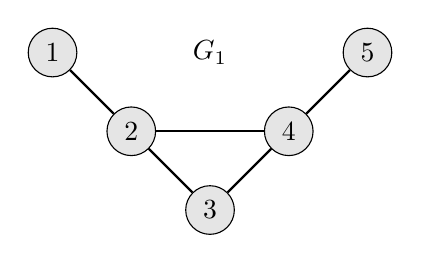
\begin{tikzpicture}[x=10mm, y=10mm]
      \node at (3,2) {$G_1$};
      \node[graph node, circle] (1) at (1,2) {1};
      \node[graph node, circle] (2) at (2,1) {2};
      \node[graph node, circle] (3) at (3,0) {3};
      \node[graph node, circle] (4) at (4,1) {4};
      \node[graph node, circle] (5) at (5,2) {5};

      \draw[thick] (1) -- (2) -- (3) -- (4) -- (5);
      \draw[thick] (2) -- (4);
    \end{tikzpicture}
    \quad\quad\quad
    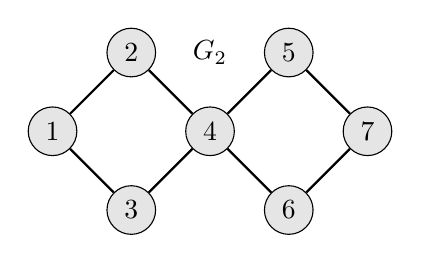
\begin{tikzpicture}[x=10mm, y=10mm]
      \node at (3,2) {$G_2$};
      \node[graph node, circle] (1) at (1,1) {1};
      \node[graph node, circle] (2) at (2,2) {2};
      \node[graph node, circle] (3) at (2,0) {3};
      \node[graph node, circle] (4) at (3,1) {4};
      \node[graph node, circle] (5) at (4,2) {5};
      \node[graph node, circle] (6) at (4,0) {6};
      \node[graph node, circle] (7) at (5,1) {7};

      \draw[thick] (4) -- (3) -- (1) -- (2) -- (4) -- (5) -- (7) -- (6) -- (4);
    \end{tikzpicture}
  \end{center}
  \end{question}
  \begin{correction}
    \begin{itemize}
    \item $\mathrm{diam}(G_1)=3$. La distance maximale est atteinte pour le couple $\langle 1, 5 \rangle$.
    \item $\mathrm{diam}(G_2)=4$. La distance maximale est atteinte pour le couple $\langle 1, 7 \rangle$.
    \end{itemize}
  \end{correction}

  \begin{question}
  \item Donner un exemple de graphe connexe à $n$ sommets de diamètre $1$, $2$ et $n-1$.
  \end{question}
  \begin{correction}
    \begin{itemize}
    \item diamètre $1$ : le graphe complet $K_n$ ;
    \item diamètre $2$ : l'étoile $S_n$ (centre + $n-1$ feuilles) ;
    \item diamètre $n-1$ : le chemin $P_n$.
    \end{itemize}
  \end{correction}

  On s'intéresse maintenant plus précisément aux deux problèmes suivants. 
  
  \Probleme{diam}{
    Un graphe $G = \langle V, E\rangle$.
  }{
    Le diamètre du graphe $G$. 
  }

  \Probleme{diam\_inf}{
    Un graphe $G = \langle V, E\rangle$, et un entier $k\in\mathbb{N}$.
  }{
    Est-ce que le diamètre du graphe $G$ est inférieur ou égal à $k$ ?
  }

  \ifcorrection{\pagebreak}
  \begin{question}
  \item Les problèmes \textsc{diam} et \textsc{diam\_inf} sont-ils des problèmes de décision ?
  \end{question}
  \begin{correction}
    Un problème de décision doit avoir une réponse binaire (\textsf{oui}/\textsf{non}).
    \textsc{diam} demande en sortie un entier, donc ce n'est pas un problème de décision.
    Par contre, \textsc{diam\_inf} est un problème de décision. 
  \end{correction}

  On suppose disposer d'un algorithme \Decide qui décide le problème \textsc{diam\_inf}.
  
  \begin{question}
  \item Proposer un algorithme déterministe \Diam qui calcule le diamètre d'un graphe $G$ en utilisant  \Decide comme sous-routine.
    On pourra utiliser le fait que, pour un graphe connexe à $n$ sommets, $0\le \Diam(G)\le n-1$.
  \end{question}
  \begin{correction}
    On peut faire une recherche linéaire, mais elle fera $n$ appels.
    On effectue ici une recherche dichotomique sur $k\in\{0,\dots,n-1\}$,
    en exploitant la monotonie de la propriété ``$\Diam(G)\le k$'' par rapport à $k$.

    \begin{algorithm}[H]
      \Fun{$\Diam(G = \langle V, E \rangle) \in \mathbb{N}$}{
        \lIf{$\lnot \Decide(G, |V|-1)$}{\Return $+\infty$;}
        $\mathit{min} \leftarrow 0$;\\
        $\mathit{max} \leftarrow |V|-1$;\\
        \While{$\mathit{min} < \mathit{max}$}{
          $\mathit{mid} \leftarrow \lfloor(\mathit{min} + \mathit{max})/2\rfloor$\;
          \lIf{$\Decide(G, \mathit{mid})$}{$\mathit{max} \leftarrow \mathit{mid}$;}
          \lElse{$\mathit{min} \leftarrow \mathit{mid}+1$;}
        }
        \Return $\mathit{min}$\;
      }
    \end{algorithm}
  \end{correction}
  

  On suppose que de plus que \Decide s'exécute en temps $\mathcal{O}\left( f(|V|, |E|) \right)$, pour une certaine fonction $f$.
  \begin{question}
  \item Donner une borne sur le nombre d'appels à la fonction \Decide effectués par l'algorithme \Diam de la question précédente,
    et en déduire la complexité totale en fonction de $f(|V|, |E|)$ et de $G$.
  \end{question}
  \begin{correction}
    \begin{enumerate}
    \item La recherche dichotomique sur un intervalle de taille $n$ effectue
      $\lceil\log_2(n)\rceil$ itérations, donc $\mathcal{O}(\log(|V|))$ appels à \Decide.

      Chaque appel à \Decide prend un temps $\mathcal{O}(f(|V|, |E|))$.
      Le reste des opérations (mise à jour des bornes, calcul du milieu, etc.)
      est polynomial par rapport au nombre de bits nécessaires pour coder un identifiant de n\oe ud,
      donc $\mathcal{O}(\log{|V|})$.
      En pratique, ce temps est négligeable par rapport à $f(|V|, |E|)$.

      On obtient donc un temps total $\mathcal{O}\left(\log(|V|) \cdot f(|V|, |E|) \right)$.
      
      Si l'on utilise une recherche linéaire, on obtient $\mathcal{O}\left(|V| \cdot f(|V|, |E|) \right)$.
    \end{enumerate}
  \end{correction}

  \begin{question}
  \item On suppose qu'il a été démontré que tout algorithme calculant $\Diam(G)$
    nécessite au moins $g(|V|, |E|)$ étapes dans le pire cas, pour une certaine fonction $g$.
    Que peut-on en déduire sur la complexité temporelle du problème $\textsc{diam\_inf}$ ?
  \end{question}
  \begin{correction}
    La complexité temporelle du problème $\textsc{diam\_inf}$ est $\Omega(\frac{g(|V|, |E|)}{\log(|V|)})$.
    
    Supposons, par contradiction, qu'il existe un algorithme qui décide $\textsc{diam\_inf}$
    en $f(|V|, |E|) < \frac{g(|V|, |E|)}{\log(|V|)}$ étapes.
    Alors notre algorithme \Diam calcule le diamètre de $G = \langle V, E\rangle$ en
    au plus

    \vspace{-2mm}
    $$\log(|V|) \cdot f(|V|, |E|) < \log(|V|) \cdot \frac{g(|V|, |E|)}{\log(|V|)} = g(|V|, |E|)$$

    \vspace{-2mm}
    étapes.
    Contradiction.
  \end{correction}
  
  \begin{question}
  \item Réciproquement, on suppose qu'il a été démontré que tout algorithme décidant
    $\textsc{diam\_inf}$ nécessite au moins $h(|V|, |E|)$ étapes dans le pire cas.
    Que peut-on en déduire sur la complexité temporelle du problème $\textsc{diam}$ ?
  \end{question}
  \begin{correction}
    \emph{Attention} : la réduction explorée dans cet exercice ne permet pas de conclure sur la
    complexité de $\textsc{diam}$. Cependant, on peut introduire une réduction dans l'autre sens.
    
    \begin{algorithm}[H]
      \Fun{$\Decide(G = \langle V, E \rangle, k \in \mathbb{N}) \in \mathbb{B}$}{
        \Return $\Diam(G) \le k$\;
      }
    \end{algorithm}

    Par le même raisonnement, on en déduit que
    la complexité temporelle de $\textsc{diam}$ est $\Omega(h(|V|, |E|))$.
  \end{correction}

  On veut maintenant définir formellement le problème \textsc{diam\_inf} comme un problème de décision sur les langages.
  On fixe l'alphabet $\Sigma = \{0,1,\#,\rightarrow\}$.
  Pour tout entier $x\in\mathbb{N}$, on note $\langle x\rangle$ son écriture binaire sans zéro initial.

  On considère l'encodage suivant des graphes simples non orientés.
  Soit $G=\langle V,E\rangle$ un graphe dont les sommets sont numérotés
  $V=\{1,\dots,n\}$.
  On encode $G$ par le mot
  $
  \langle G\rangle \eqdef
  \langle n\rangle
  \#
  \langle u_1\rangle \rightarrow \langle v_1\rangle
  \# \cdots \#
  \langle u_m\rangle \rightarrow \langle v_m\rangle,
  $
  où chaque arête $\{u_i,v_i\}\in E$ est écrite exactement une fois, avec la convention
  $1 \le u_i < v_i \le n$.
  L'ordre des arêtes est arbitraire.

  \begin{question}
  \item Donnez un encodage du graphe $G_1$ dans ce langage.
  \end{question}
  \begin{correction}
    $\langle G_1 \rangle = 101\#1\rightarrow10\#10\rightarrow11\#11\rightarrow100\#100\rightarrow101\#10\rightarrow100$
  \end{correction}

  \begin{question}
    \item Définissez le langage $L_{\textsc{diam\_inf}}$ des encodages des instances positives du problème \textsc{diam\_inf}.
  \end{question}
  \begin{correction}
    $L_{\textsc{diam\_inf}} \eqdef \{ \langle G \rangle \# \langle k \rangle \mid \mathrm{diam}(G) \le k \}$.
  \end{correction}

  \begin{question}
  \item En déduire une borne sur la complexité de \Diam en fonction de $f$ et de la taille de son entrée. 
  \end{question}
  \begin{correction}
    Dans l'encodage choisi, on a $|\langle n\rangle| = \Theta(\log n)$ et,
    pour chaque arête, $|\langle u_i\rangle|$ et $|\langle v_i\rangle|$ valent $\Theta(\log n)$, puisque $1\le u_i,v_i\le n$.
    Chaque arête contribue donc $\Theta(\log n)$ bits (à une constante près), et les séparateurs contribuent $O(1)$.
    Ainsi, $|\langle G \rangle \# \langle k \rangle| = \Theta(\log(n) + m\log(n) + \log(n)) = \Theta(m\log n)$.

    On peut réécrire la complexité obtenue uniquement en fonction de la taille $s$ de l'entrée.
    L'algorithme \Diam s'exécute donc en temps
    $\mathcal{O}\left(\log(s) \cdot f(s, s)\right)$.
  \end{correction}
  
\end{exercice}

\endgroup
\endinput

 
 
\session{Machines de Turing déterministes}
% SPDX-License-Identifier: CC-BY-SA-4.0
% Author: Matthieu Perrin
% Part: Turing machines
% Section: Deterministic Turing machines
% Exercise: Executions of a Turing machine

\begingroup
\begin{exercice}[Exécution d'une machine de Turing]\label{exo:turingmachines/definitions/executions}
  
  On se donne la machine de Turing déterministe $M$ suivante sur l'alphabet $\Sigma = \{a, b\}$. 

  \begin{center}
    \begin{tikzpicture}[turingMachine, x=30mm, y=15mm]
      \state[initial]   (0) at (5,1) {$0$};
      \state            (1) at (4,0) {$1$};
      \state            (2) at (5,0) {$2$};
      \state            (3) at (6,0) {$3$};
      \state[accepting] (4) at (6,1) {$4$};
      
      \path (0) edge             node[sloped] {\smTMtransR{a}{c}} (1);
      \path (1) edge[loop below] node         {\smAlign{\smTMtransR{a}{a}\smTMtransR{c}{c}}} (1);
      \path (1) edge             node         {\smTMtransL{b}{c}} (2);
      \path (2) edge[loop below] node         {$\begin{array}{c}\smTMtransL{x}{x} \\ \forall x\in \{a, b, c\}\end{array}$} (2);
      \path (2) edge             node[sloped] {\smTMtransR{\blank}{\blank} } (0);
      \path (0) edge             node[sloped] {\smTMtransR{b}{c}} (3);
      \path (3) edge[loop below] node         {\smAlign{\smTMtransR{b}{b}\smTMtransR{c}{c}}} (3);
      \path (3) edge             node[swap]   {\smTMtransL{a}{c}} (2);
      \path (0) edge[loop above] node         {\smTMtransR{c}{c}} (0);
      \path (0) edge             node         {\smTMtransR{\blank}{\blank}} (4);
    \end{tikzpicture}
  \end{center}
  
  \begin{question}
  \item Donnez la suite des configurations de l'exécution de $M$ sur $abab$ et sur $aaba$.
  \end{question}
  \begin{correction}
    
    $\begin{array}{rc@{\quad \langle\,}r@{,~}c@{,~}l@{\,\rangle}}
      C_{\mathit{init}}(abab)
      & =        & \varepsilon & 0 & abab        \\
      & \leadsto & c           & 1 & bab         \\
      & \leadsto & \varepsilon & 2 & ccab        \\
      & \leadsto & \varepsilon & 2 & \blank ccab \\
      & \leadsto & \varepsilon & 0 & ccab        \\
      & \leadsto & c           & 0 & cab         \\
      & \leadsto & cc          & 0 & ab          \\
      & \leadsto & ccc         & 1 & b           \\
      & \leadsto & cc          & 2 & cc          \\
      & \leadsto & c           & 2 & ccc         \\
      & \leadsto & \varepsilon & 2 & cccc        \\
      & \leadsto & \varepsilon & 2 & \blank cccc \\
      & \leadsto & \varepsilon & 0 & cccc        \\
      & \leadsto & c           & 0 & ccc         \\
      & \leadsto & cc          & 0 & cc          \\
      & \leadsto & ccc         & 0 & c           \\
      & \leadsto & cccc        & 0 & \varepsilon \\
      & \leadsto & cccc\blank  & 4 & \varepsilon \\
    \end{array}$
    $\begin{array}{rc@{\quad \langle\,}r@{,~}c@{,~}l@{\,\rangle}}
      C_{\mathit{init}}(aaba)
      & =        & \varepsilon & 0 & aaba        \\
      & \leadsto & c           & 1 & aba         \\
      & \leadsto & ca          & 1 & ba          \\
      & \leadsto & c           & 2 & aca         \\
      & \leadsto & \varepsilon & 2 & caca        \\
      & \leadsto & \varepsilon & 2 & \blank caca \\
      & \leadsto & \varepsilon & 0 & caca        \\
      & \leadsto & c           & 0 & aca         \\
      & \leadsto & cc          & 1 & ca          \\
      & \leadsto & ccc         & 1 & a           \\
      & \leadsto & ccca        & 1 & \varepsilon \\
    \end{array}$
  \end{correction}
  
  \begin{question}
  \item Les mots $abab$ et $aaba$ sont-ils acceptés par $M$ ? 
  \end{question}
  \begin{correction}
    $abab$ est accepté,  mais $aaba$ est rejeté
  \end{correction}
  
  \begin{question}
  \item Quel est le langage reconnu par $M$ ? 
  \end{question}
  \begin{correction}
    $\{u \in \{a, b\}^\star \mid |u|_a = |u|_b \}$
  \end{correction}

\end{exercice}

\endgroup
\endinput

% SPDX-License-Identifier: CC-BY-SA-4.0
% Author: Matthieu Perrin
% Part: Turing machines
% Section: Deterministic Turing machines
% Exercise: Conception of Turing machines

\begingroup

\begin{exercice}[Conception de machines de Turing]\label{exo:turingmachines/definitions/languages}

  Dans cet exercice, on se limitera au modèle strict des machines de Turing sur un seul ruban. 

  \begin{question}
  \item Construire une machine de Turing déterministe qui décide le langage $\{ w c w \mid w\in \{a, b\}^\star \}$.
  \end{question}
  \begin{correction}
    \begin{tikzpicture}[turingMachine, baseline=(0)]
      \state[initial above] (0) at (2,1) {$0$}; 
      \state                (1) at (3,2) {$1$}; 
      \state                (2) at (4,2) {$2$}; 
      \state                (3) at (3,0) {$3$}; 
      \state                (4) at (4,0) {$4$}; 
      \state                (5) at (5,1) {$5$}; 
      \state                (6) at (1,1) {$6$}; 
      \state[accepting]     (7) at (0,1) {$7$}; 

      \path (0) edge  node       {\smTMtransR{a}{\blank}}      (1);
      \path (1) edge  node       {\smTMtransR{c}{c}}           (2);
      \path (2) edge  node       {\smTMtransL{a}{X}}           (5);
      \path (0) edge  node[swap] {\smTMtransR{b}{\blank}}      (3);
      \path (3) edge  node[swap] {\smTMtransR{c}{c}}           (4);
      \path (4) edge  node[swap] {\smTMtransL{b}{X}}           (5);
      \path (5) edge  node[swap] {\smTMtransR{\blank}{\blank}} (0);
      \path (0) edge  node[swap] {\smTMtransR{c}{c}}           (6);
      \path (6) edge  node[swap] {\smTMtransL{\blank}{\blank}} (7);

      \path (1) edge[loop above] node {\smAlign{\smTMtransR{a}{a}\smTMtransR{b}{b}}}                                   (1);
      \path (2) edge[loop above] node {\smTMtransR{X}{X}}                                                              (2);
      \path (3) edge[loop below] node {\smAlign{\smTMtransR{a}{a}\smTMtransR{b}{b}}}                                   (3);
      \path (4) edge[loop below] node {\smTMtransR{X}{X}}                                                              (4);
      \path (5) edge[loop right] node {\smAlign{\smTMtransL{a}{a}\smTMtransL{b}{b}\smTMtransL{c}{c}\smTMtransL{X}{X}}} (5);
      \path (6) edge[loop above] node {\smTMtransR{X}{X}}                                                              (6);

    \end{tikzpicture}
  \end{correction}
  
  \begin{question}
  \item Construire une machine de Turing déterministe qui génère le langage $\{a^n b^n a^n \mid n \ge 0\}$.
  \end{question}
  \begin{correction}
    \begin{tikzpicture}[turingMachine, baseline=(1), y=20mm]
      \state[initial]   (0) at (0,1) {$0$}; 
      \state            (1) at (1,1) {$1$}; 
      \state            (2) at (2,1) {$2$}; 
      \state[accepting] (3) at (3,1) {$3$}; 
      \state            (4) at (3,0) {$4$}; 
      \state            (5) at (2,0) {$5$}; 
      \state            (6) at (1,0) {$6$}; 

      \path (0) edge             node {\smTMtransR{\blank}{a}}                       (1);
      \path (1) edge             node {\smTMtransR{\blank}{b}}                       (2);
      \path (2) edge             node {\smTMtransL{\blank}{a}}                       (3);
      \path (3) edge[loop right] node {\smAlign{\smTMtransL{a}{a}\smTMtransL{b}{b}}} (3);
      \path (3) edge             node {\smTMtransR{\blank}{a}}                       (4);
      \path (4) edge[loop below] node {\smTMtransR{a}{a}}                            (4);
      \path (4) edge             node {\smTMtransR{b}{b}}                            (5);
      \path (5) edge[loop below] node {\smTMtransR{b}{b}}                            (5);
      \path (5) edge             node {\smTMtransR{a}{b}}                            (6);
      \path (6) edge[loop below] node {\smTMtransR{a}{a}}                            (6);
      \path (6) edge             node {\smTMtransR{\blank}{a}}                       (2);
    \end{tikzpicture}
  \end{correction}

  \begin{question}
  \item Construire une machine de Turing déterministe qui décide le langage $\{ a^{2^n} \mid n \ge 0 \}$.
  \end{question}
  \begin{correction}
    \begin{tikzpicture}[turingMachine, baseline=(0)]
      \state                (0) at (0,0) {$0$}; 
      \state[initial above] (1) at (1,0) {$1$}; 
      \state                (2) at (2,0) {$2$}; 
      \state                (3) at (3,0) {$3$}; 
      \state[accepting]     (4) at (4,0) {$4$}; 

      \path (0) edge[bend left]  node {\smTMtransR{\blank}{\blank}} (1);
      \path (1) edge[bend left]  node {\smTMtransL{\blank}{\blank}} (0);
      \path (2) edge[bend left]  node {\smTMtransR{a}{a}} (1);
      \path (1) edge[bend left]  node {\smTMtransR{a}{A}} (2);
      \path (2) edge             node {\smTMtransL{\blank}{\blank}} (3);
      \path (3) edge             node {\smTMtransR{\blank}{\blank}} (4);
      \path (0) edge[loop left]  node {\smAlign{\smTMtransL{a}{a}\smTMtransL{A}{A}}} (0);
      \path (1) edge[loop below] node {\smTMtransR{A}{A}} (1);
      \path (2) edge[loop below] node {\smTMtransR{A}{A}} (2);
      \path (3) edge[loop below] node {\smTMtransL{A}{A}} (3);
    \end{tikzpicture}
  \end{correction}
  
\end{exercice}

\endgroup
\endinput

% SPDX-License-Identifier: CC-BY-SA-4.0
% Author: Matthieu Perrin
% Part: Turing machines
% Section: Deterministic Turing machines
% Exercise: Tape exploration

\begingroup

\begin{exercice}[Exploration de ruban]\label{exo:turingmachines/definitions/exploration}

  L'objectif de cet exercice est de concevoir des machines de Turing capables de localiser le début d'un mot $w$ sur un ruban.
  Initialement, le ruban contient un mot $w\in \{a\}^+$ entouré de cases vides $\blank$,
  et la tête de lecture peut commencer sur une position arbitraire, potentiellement éloignée à gauche ou à droite du mot $w$.
  La machine de Turing doit atteindre une configuration bloquante dans laquelle la tête de lecture se trouve au début du mot $w$. 

  \begin{question}
  \item Construisez une machine de Turing déterministe $M$ qui localise le début du mot $w$.
  \end{question}
  \begin{correction}
    \begin{tikzpicture}[turingMachine, baseline=(0)]
      \state[initial above] (0) at (0,0) {$0$}; 
      \state                (1) at (1,0) {$1$}; 
      \state[accepting]     (2) at (2,0) {$2$};

      \path (0) edge[loop left]  node {\smAlign{\smTMtransL{a}{a}\smTMtransL{b}{b}}} (0);
      \path (0) edge[bend left]  node {\smTMtransR{\blank}{b}}                       (1);
      \path (1) edge[bend left]  node {\smTMtransL{\blank}{b}}                       (0);
      \path (1) edge[loop above] node {\smTMtransR{b}{b}}                            (1);
      \path (1) edge             node {\smTMtransS{a}{a}}                            (2);
    \end{tikzpicture}
  \end{correction}

  \begin{question}
  \item Que se passe-t-il si $w\in \{a\}^\star$ ?
  \end{question}
  \begin{correction}
    La machine $M_{d}$ ne termine pas sur le mot $\varepsilon$. 
  \end{correction}

\end{exercice}

\endgroup
\endinput

 
 
\session{Expressivité des machines de Turing}
% SPDX-License-Identifier: CC-BY-SA-4.0
% Author: Matthieu Perrin
% Part: Turing machines
% Section: Epressiveness of Turing machines
% Exercise: Computable function 

\begingroup

\begin{exercice}[Calculabilité de la fonction \texttt{CaractereEn(u,i)}]\label{exo:turingmachines/expressiveness/at}

  \SetKwFunction{CaractereEn}{CaractereEn}

  \begin{question}
  \item Donnez une machine de Turing qui prend en entrée un nombre entier $i$ écrit en binaire sur un ruban \textsc{i}
    et un mot $u \in \Sigma^\star$ sur un ruban \textsc{u},
    et écrit sur le ruban \textsc{c} le $i^{\text{e}}$ caractère de $u$ (on supposera $|u| \ge i$).
  \end{question}

  \begin{correction}
    La principale difficulté est de traduire $i$ en unaire, pour pouvoir déplacer le tête de lecture sur $u$. Une façon de faire est par décrémentations successives de $i$.

    \begin{algorithm}[H]
      \Fun{$\CaractereEn(u,i)$}{
        \While{$i\neq 0$}{
          $i \leftarrow i-1$;\\
          $u \leftarrow \&u[1]$; \tcp{$\textsc{u}:\smTMtransR{x}{x}$}
        }
        $c \leftarrow u[0]$; \tcp{$\textsc{u}:\smTMtransS{x}{x}, \textsc{c}:\smTMtransS{\blank}{x} $}
      }    
    \end{algorithm}

    \begin{center}
      \begin{tikzpicture}[turingMachine, x=30mm]
        \state[initial left] (0) at (0,0) {$0$}; 
        \state               (1) at (1,0) {$1$}; 
        \state[accepting]    (2) at (2,0) {$2$}; 

        \path (0) edge[loop above] node       {\smAlign{\smTMtransR[\textsc{i}]{0}{0}\smTMtransR[\textsc{i}]{1}{1}}} (0);
        \path (1) edge[loop above] node       {\smTMtransL[\textsc{i}]{0}{1}}                                        (1);
        \path (0) edge[bend left]  node       {\smTMtransL[\textsc{i}]{\blank}{\blank}}                              (1);
        \path (1) edge[bend left]  node       {\smGroup{\smTMtransR[\textsc{i}]{1}{0}\smTMtransR[\textsc{u}]{x}{x}}} (0);
        \path (1) edge             node[swap] {\smGroup{\smTMtransL[\textsc{i}]{\blank}{\blank}\smTMtransS[\textsc{u}]{x}{x}\smTMtransS[\textsc{c}]{\blank}{x}}} (2);
      \end{tikzpicture}
      $\forall x\in \Sigma$
    \end{center}
  \end{correction}
  
\end{exercice}

\endgroup
\endinput

% SPDX-License-Identifier: CC-BY-SA-4.0
% Author: Matthieu Perrin
% Part: Turing machines
% Section: Epressiveness of Turing machines
% Exercise: Models of Turing machines

\begingroup

\begin{exercice}[Modèles de machines de Turing]\label{exo:turingmachines/expressiveness/models}

  Le but de cet exercice est de comparer deux modèles de machines de Turing :
  \begin{itemize}
    \item le modèle strict, à un seul ruban, et qui ne permet que de lire et d'écrire dans les cases du ruban ; 
    \item et le modèle étendu vu en cours, à plusieurs rubans, qui autorise en plus l'insertion et la suppression de cases sur les rubans.
  \end{itemize}

  \begin{question}
  \item Construire une machine du modèle étendu qui décide le langage $\{ww^\textsc{r} \mid w \in \{a, b\}^\star\}$.
  \end{question}
  \begin{correction}
    \begin{tikzpicture}[turingMachine, baseline=(0), x=30mm]
      \state[initial]   (0) at (0,0) {$0$}; 
      \state            (1) at (1,0) {$1$}; 
      \state            (2) at (2,0) {$2$}; 
      \state[accepting] (3) at (3,0) {$3$}; 
 
      \path (0) edge[loop above]  node {\smGroup{\smTMtransR[\textsc{i}]{x}{x}\smTMtransR[\textsc{a}]{\blank}{x}}} (0);
      \path (0) edge              node {\smGroup{\smTMtransL[\textsc{i}]{\blank}{\blank}\smTMtransL[\textsc{a}]{\blank}{\blank}}} (1);
      \path (1) edge[loop above]  node {\smTMtransL[\textsc{i}]{x}{x}}           (1);
      \path (1) edge              node {\smTMtransR[\textsc{i}]{\blank}{\blank}}      (2);
      \path (2) edge[loop above]  node {\smGroup{\smTMtransR[\textsc{i}]{x}{x}\smTMtransL[\textsc{a}]{x}{x}}} (2);
      \path (2) edge              node {\smGroup{\smTMtransL[\textsc{i}]{\blank}{\blank}\smTMtransR[\textsc{a}]{\blank}{\blank}}} (3);
    \end{tikzpicture}
  \end{correction}

  \begin{question}
  \item Construire une machine du modèle strict qui décide le langage $\{ww^\textsc{r} \mid w \in \{a, b\}^\star\}$.
  \end{question}
  \begin{correction}
    \begin{tikzpicture}[turingMachine, baseline=(1), y=12mm]
      \state[initial above] (0) at (1,1) {$0$}; 
      \state                (1) at (2,2) {$1$}; 
      \state                (2) at (3,2) {$2$}; 
      \state                (3) at (2,0) {$3$}; 
      \state                (4) at (3,0) {$4$}; 
      \state                (5) at (4,1) {$5$}; 
      \state[accepting]     (6) at (0,1) {$6$}; 

      \path (1) edge[loop left]  node               {\smAlign{\smTMtransR{a}{a}\smTMtransR{b}{b}}} (1);
      \path (3) edge[loop left]  node               {\smAlign{\smTMtransR{a}{a}\smTMtransR{b}{b}}} (3);
      \path (5) edge[loop right] node               {\smAlign{\smTMtransL{a}{a}\smTMtransL{b}{b}}} (5);
      \path (0) edge             node[sloped, swap] {\smTMtransR{a}{\blank}}                       (1);
      \path (1) edge             node[sloped]       {\smTMtransL{\blank}{\blank}}                  (2);
      \path (2) edge             node[sloped, swap] {\smTMtransL{a}{\blank}}                       (5);
      \path (0) edge             node[sloped]       {\smTMtransR{b}{\blank}}                       (3);
      \path (3) edge             node[sloped]       {\smTMtransL{\blank}{\blank}}                  (4);
      \path (4) edge             node[sloped]       {\smTMtransL{b}{\blank}}                       (5);
      \path (5) edge             node[sloped]       {\smTMtransR{\blank}{\blank}}                  (0);
      \path (0) edge             node[sloped]       {\smTMtransR{\blank}{\blank}}                  (6);
    \end{tikzpicture}
  \end{correction}

  \begin{question}
  \item Construire une machine du modèle étendu qui décide le langage $\{a^{n^2} \mid n\in \mathbb{N} \}$.
    
    \emph{Remarque :} on rappelle que $\sum_{k=0}^n (2k+1) = (n+1)^2$.
  \end{question}
  \begin{correction}
    \begin{tikzpicture}[turingMachine, baseline=(0), x=40mm]
      \state                (2) at (0,0) {$2$}; 
      \state                (1) at (1,0) {$1$}; 
      \state[initial above] (0) at (2,0) {$0$}; 
      \state[accepting]     (3) at (3,0) {$3$}; 

      \path (1) edge[loop below]   node {\smGroup{\smTMtransR[\textsc{i}]{a}{a}\smTMtransR[\textsc{k}]{1}{1}}} (1);
      \path (2) edge[loop below]   node {\smGroup{\smTMtransR[\textsc{i}]{a}{a}\smTMtransL[\textsc{k}]{1}{1}}} (2);
      \path (0) edge               node {\smTMtransR[\textsc{i}]{a}{a}}                                        (1);
      \path (1) edge               node {\smTMtransL[\textsc{k}]{\blank}{\blank}}                              (2);
      \path (2) edge[bend left=15] node {\smTMtransS[\textsc{k}]{\blank}{1}}                                   (0);
      \path (0) edge               node {\smTMtransL[\textsc{i}]{\blank}{\blank}}                              (3);
    \end{tikzpicture}
  \end{correction}

  \begin{question}
  \item Construire une machine du modèle étendu qui décide le langage de Dyck : $\mathcal{L}(S \rightarrow (S) \mid SS \mid \varepsilon)$.
  \end{question}
  \begin{correction}
    \vspace{-2mm}
    \begin{tikzpicture}[turingMachine, baseline=(0), x=30mm]
      \state[initial]   (0) at (0,0) {$0$}; 
      \state            (1) at (1,0) {$1$}; 
      \state            (2) at (2,0) {$2$}; 
      \state[accepting] (3) at (3,0) {$3$}; 

      \path (0) edge             node {\smTMtransR[\textsc{c}]{x}{x}}                                                            (1);
      \path (1) edge[loop above] node {\smGroup{\smTMtransR[\textsc{i}]{(}{(}\smTMtransR[\textsc{c}]{\blank}{\blank}}}           (1);
      \path (1) edge[loop below] node {\smGroup{\smTMtransR[\textsc{i}]{)}{)}\smTMtransL[\textsc{c}]{\blank}{\blank}}}           (1);
      \path (1) edge             node {\smGroup{\smTMtransL[\textsc{i}]{\blank}{\blank}\smTMtransL[\textsc{c}]{\blank}{\blank}}} (2);
      \path (2) edge             node {\smTMtransS[\textsc{c}]{x}{x}}                                                            (3);
    \end{tikzpicture}
    \vspace{-2mm}
  \end{correction}
  
\end{exercice}

\endgroup
\endinput

 
 
\session{Thèse de Church-Turing}
% SPDX-License-Identifier: CC-BY-SA-4.0
% Author: Matthieu Perrin
% Part: Introduction
% Section: Words and languages
% Exercise: Words

\begingroup

\tikzset{
  sub tm/.style={fill=black!20, rounded corners=7, inner sep=0pt, minimum height=1cm, minimum width=1cm,},
  tm state/.style={fill=black!20,},
}

\begin{exercice}[Calculabilité d'un langage impératif]\label{exercice:IMPtoMT}

  On considère un petit langage impératif, \emph{IMP}, dont les seules données manipulées sont des \emph{chaînes de caractères} sur un alphabet $\Gamma$.
  La syntaxe du langage est donnée par la grammaire\footnote{La grammaire est volontairement simplifiée et ambigüe} suivante,
  dans laquelle le non-terminal \textsc{i} représente les instructions,
  le non-terminal \textsc{x} les identifiants de variable,
  et le non-terminal \textsc{c} les chaînes de caractères constantes.
  Le langage ne contient volontairement pas d'expressions complexes pour en simplifier l'analyse. 
  
  $$\left\{\begin{array}{rcll}
  \textsc{i} & \rightarrow & \texttt{skip}                                                                                           & \text{ne rien faire}\\
  &                \mid        & \textsc{i} ; \textsc{i}                                                                             & \text{exécution séquentielle}\\
  &                \mid        & \texttt{if }\textsc{x}\neq\textsc{x}\texttt{ then }\textsc{i}\texttt{ else }\textsc{i}\texttt{ end} & \text{conditionnelle}\\
  &                \mid        & \texttt{while }\textsc{x}\neq\textsc{x}\texttt{ do }\textsc{i}\texttt{ end}                         & \text{boucle}\\
  &                \mid        & \textsc{x} \leftarrow `` \textsc{c} "                                                               & \text{affectation d'une constante}\\
  &                \mid        & \textsc{x} \leftarrow \textsc{x}                                                                    & \text{affectation d'une copie}\\
  &                \mid        & \textsc{x} \leftarrow \textsc{x} + \textsc{x}                                                       & \text{affectation de la concaténation}\\
  &                \mid        & \textsc{x} \leftarrow \texttt{head}(\textsc{x})                                                     & \text{affectation du premier caractère}\\
  &                \mid        & \textsc{x} \leftarrow \texttt{tail}(\textsc{x})                                                     & \text{affectation des caractères suivants}\\
  \textsc{x} & \rightarrow & [a-z]^+                                                                                                 & \text{nom de variable}\\
  \textsc{c} & \rightarrow & \Gamma^\star                                                                                             & \text{chaîne de caractères constante}\\
  \end{array}\right.$$
  
  On considère la sémantique standard des instructions, où \texttt{head} et \texttt{tail} désignent respectivement
  le premier symbole et le reste d'une chaîne, et \texttt{+} la concaténation.
  
  On suppose que les données d'entrées du programme sont stockées dans une variable spéciale $\mathit{input}$,
  et la sortie du programme est la valeur stockée dans la variable spéciale $\mathit{output}$ lorsque le programme s'arrête sans erreur.
  En cas de boucle infinie ou d'erreur (par exemple lors de la lecture d'une variable non initialisée ou de l'appel à \texttt{head} ou \texttt{tail} sur une chaîne vide),
  on considère que la sortie est indéfinie.
  La \emph{fonction calculée} par le programme est alors définie comme la fonction partielle
  de $\Gamma^\star$ vers $\Gamma^\star$ qui associe à chaque entrée la sortie produite par le programme.
  
  Par exemple, les programmes suivants calculent respectivement la fonction miroir et la projection sur ``a'' :

  $$
  \begin{array}{l}
    \mathit{empty}~\leftarrow ``" ;\\
    \mathit{output}\leftarrow \mathit{empty} ;\\
    \texttt{while }\mathit{input} \neq \mathit{empty} \texttt{ do } \\
    \quad  \mathit{tmp} ~~~~~\leftarrow \texttt{head}(\mathit{input}) ;\\
    \quad  \mathit{output} \leftarrow \mathit{tmp} + \mathit{output} ;\\
    \quad  \mathit{input} ~~\leftarrow \texttt{tail}(\mathit{input})\\
    \texttt{end}
  \end{array}
  \quad\quad\quad
  \begin{array}{l}
    \mathit{empty}\leftarrow ``" ; \mathit{output}\leftarrow \mathit{empty} ; \mathit{a}\leftarrow ``a" ; \\
    \texttt{while }\mathit{input} \neq \mathit{empty} \texttt{ do } \\
    \quad  \mathit{tmp} ~~~\leftarrow \texttt{head}(\mathit{input}) ;\\
    \quad  \mathit{input} \leftarrow \texttt{tail}(\mathit{input})\\
    \quad  \texttt{if }\mathit{tmp} \neq \mathit{a} \texttt{ then skip else } \\
    \quad\quad  \mathit{output} \leftarrow \mathit{output} + \mathit{tmp} \\
    \quad  \texttt{end }\\
    \texttt{end}
  \end{array}
  $$

  On cherche à montrer que le langage IMP est au moins aussi puissant que le modèle des machines de Turing.
  Pour cela, on considère une machine de Turing déterministe
  $M = \langle \Sigma, \Gamma, \blank, Q, q_0, F, \rightarrow \rangle$,
  et on se donne pour objectif de construire un programme IMP qui simule les exécutions de $M$.
  On supposera que les états de la machine sont encodés par des mots sur $\Gamma$,
  c'est-à-dire que $Q \subset \Gamma^+$.

  Dans toute la construction qui suit, on imposera les invariants suivants.
  On utilisera trois variables $\mathit{state}$, $\mathit{left}$ et $\mathit{right}$
  pour représenter une configuration de $M$ sous la forme
  $\langle \mathit{left}, \mathit{state}, \mathit{right} \rangle$,
  où :
  \begin{itemize}
  \item la partie gauche du ruban est encodée en miroir, de sorte que
    $\texttt{head}(\mathit{right})$ désigne le symbole actuellement sous la tête de lecture,
    et $\texttt{head}(\mathit{left})$ le symbole immédiatement à sa gauche ;
  \item le dernier caractère de $\mathit{left}$ et de $\mathit{right}$ est toujours
    le symbole blanc $\blank$.
  \end{itemize}

  \pagebreak
  
  \begin{question}
  \item Proposer un programme IMP qui initialise la configuration $\langle \mathit{left}, \mathit{state}, \mathit{right} \rangle$
    en fonction de $\mathit{input}$.
  \end{question}
  \begin{correction}
    $\mathit{left} \leftarrow ``" ; \mathit{state} \leftarrow q_0 ; \mathit{right} \leftarrow \mathit{input}$
  \end{correction}
  
  \begin{question}
  \item On considère une transition $ q\xrightarrow{\smTMtransR{a}{b}} q'$ de $M$.
    Proposer un programme IMP qui vérifie si la transition peut être tirée,
    et si oui modifie les variables $\mathit{state}$, $\mathit{left}$ et $\mathit{right}$
    en conséquence.
  \end{question}
  \begin{correction}
    $$\begin{array}{l}
      \mathit{empty} \leftarrow ``" ; \mathit{blank} \leftarrow ``\blank" ;\\
      \mathit{tstate}~\leftarrow q ;
      \mathit{tchar}~\leftarrow a ;
      \mathit{trans}~\leftarrow \mathit{tstate} + \mathit{tchar} ;\\
      \mathit{hd}~\leftarrow \texttt{head}(\mathit{right}) ;
      \mathit{curr}~\leftarrow \mathit{state} + \mathit{hd} ;\\
      \texttt{if }\mathit{trans} \neq \mathit{curr} \texttt{ then }\\
      \quad \texttt{skip} \\
      \texttt{else} \\
      \quad \mathit{left}~ \leftarrow \mathit{left} + \mathit{hd} ;\\
      \quad \mathit{state} \leftarrow q' ;\\
      \quad \mathit{right} \leftarrow \texttt{tail}(\mathit{right}) ;\\
      \quad \texttt{if }\mathit{right} \neq \mathit{empty} \texttt{ then skip else } \mathit{right} \leftarrow \mathit{right} + \mathit{blank} \texttt{ end}\\
      \texttt{end}
    \end{array}$$
  \end{correction}
  
  \begin{question}
  \item En déduire un programme IMP qui simule les exécutions de la machine de Turing suivante.
    On veillera en particulier à initialiser la variable $\mathit{output}$
    en fonction de la configuration $\langle \mathit{left}, \mathit{state}, \mathit{right} \rangle$.
    
    \begin{tikzpicture}[turingMachine, baseline=(a.base)]
      \state[initial]   (a) at (0,0) {$0$}; 
      \state[accepting] (b) at (1,0) {$1$}; 
      \path (a) edge[loop above] node {\smTMtransR{1}{0}} (a);
      \path (a) edge             node {\smTMtransL{0}{1}} (b);
    \end{tikzpicture}
  \end{question}
  \begin{correction}

    $$\begin{array}{l}
      \mathit{empty} \leftarrow ``" ; \mathit{blank} \leftarrow ``\blank" ; \mathit{done} \leftarrow \mathit{empty};\\
      \texttt{while }\mathit{done} \neq \mathit{blank} \texttt{ do }\\
      \quad \mathit{hd}~\leftarrow \texttt{head}(\mathit{right}) ;
      \quad \mathit{curr}~\leftarrow \mathit{state} + \mathit{hd} ;\\
      \quad \mathit{trans}~\leftarrow ``01" ;\\
      \quad \texttt{if }\mathit{trans} \neq \mathit{curr} \texttt{ then }\\
      \quad \quad \mathit{trans}~\leftarrow ``00" ;\\
      \quad \quad \texttt{if }\mathit{trans} \neq \mathit{curr} \texttt{ then }\\
      \quad \quad \quad \mathit{done} \leftarrow \mathit{blank}; \\
      \quad \quad \texttt{else} \\
      \quad \quad \quad \mathit{hd}~\leftarrow \texttt{head}(\mathit{left}) ; \\
      \quad \quad \quad \mathit{left} \leftarrow \texttt{tail}(\mathit{left}) ;\\
      \quad \quad \quad \texttt{if }\mathit{left} \neq \mathit{empty} \texttt{ then skip else } \mathit{left} \leftarrow \mathit{left} + \mathit{blank} \texttt{ end}\\
      \quad \quad \quad \mathit{state} \leftarrow 1 ;\\
      \quad \quad \quad \mathit{right}~ \leftarrow \mathit{right} + \mathit{hd} ;\\
      \quad \quad \texttt{end} \\
      \quad \texttt{else} \\
      \quad \quad \mathit{left}~ \leftarrow \mathit{left} + \mathit{hd} ;\\
      \quad \quad \mathit{state} \leftarrow 0 ;\\
      \quad \quad \mathit{right} \leftarrow \texttt{tail}(\mathit{right}) ;\\
      \quad \quad \texttt{if }\mathit{right} \neq \mathit{empty} \texttt{ then skip else } \mathit{right} \leftarrow \mathit{right} + \mathit{blank} \texttt{ end}\\
      \quad \texttt{end}\\
      \texttt{end}
      \mathit{output} \leftarrow \mathit{right} ;\\
      \texttt{while } \mathit{left} \neq \mathit{empty} \texttt{ do }\\
      \quad \mathit{tmp} \leftarrow \texttt{head}(\mathit{left}) ; \mathit{output} \leftarrow \mathit{tmp} + \mathit{output} ; \mathit{left} \leftarrow \texttt{tail}(\mathit{left})\\
      \texttt{end}
    \end{array}$$
  \end{correction}
  
  On cherche maintenant à établir la réciproque du résultat précédent :
  toute exécution d’un programme IMP $P$ peut être simulée par une machine de Turing déterministe $M(P)$.
  Pour cela, on va construire la machine $M(P)$ par induction structurelle sur l'arbre de syntaxe abstraite du programme $P$.

  Les différentes machines construites vont vérifier les invariants suivants :
  
  \begin{itemize}
  \item $M(P)$ possède un ruban différent associé à chaque variable utilisée par le programme $P$,
    y compris les rubans $\mathit{input}$ où est marquée la valeur d'entrée et $\mathit{output}$
    où est lue la valeur de sortie.
  \item
    $M(P)$ peut posséder des rubans de travail supplémentaires (nommés $1$, $2$, etc) que vous pouvez introduire à votre guise.
  \item $M(P)$ possède un unique état accepteur $q_+$, d'où aucune transition ne sort. 
  \item Dans l'état accepteur $q_+$, toutes les têtes de lecture sont positionnées au début du mot de leur ruban respectif.
  \end{itemize}
  
  On représentera la machine de Turing $M(P)$ par : 
  \begin{tikzpicture}[turingMachine, baseline=(a.base)]
    \state[tm state, initial]   (a) at (2,3) {$q_0^P$}; 
    \state[tm state, accepting] (b) at (4,3) {$q_+^P$}; 
    \path[dashed] (a) edge node{\footnotesize $M(P)$} (b);
    
    \begin{pgfonlayer}{background}%
      \node[sub tm, fit=(a.center)(b.center)]         {};
    \end{pgfonlayer}%
  \end{tikzpicture}


  \begin{question}
  \item Étant données deux variables $x$ et $y$, construire les machines
    de Turing qui mène dans deux états distincts $q_+$ et $q_-$
    en fonction de l'égalité des mots stockés sur les rubans
    \textsc{x} et \textsc{y}.
  \end{question}
  \begin{correction}
    \vspace{-4mm}
    \begin{tikzpicture}[turingMachine, baseline=(0.base), x=30mm, y=10mm]
    \state[initial above] (0) at (2,0) {$q_0$}; 
    \state                (1) at (1,0) {}; 
    \state                (2) at (0,0) {$q_+$}; 
    \state                (3) at (3,0) {}; 
    \state                (4) at (4,0) {$q_-$}; 

    \path   (0) edge[loop below] node      {\smGroup{\smTMtransR[\textsc{x}]{x}{x}\smTMtransR[\textsc{y}]{x}{x}} }                         (0);
    \path   (0) edge             node      {\smGroup{\smTMtransL[\textsc{x}]{\blank}{\blank}\smTMtransL[\textsc{y}]{\blank}{\blank}} }     (1);
    \path   (1) edge[loop below] node      {\smGroup{\smTMtransL[\textsc{x}]{x}{x}\smTMtransL[\textsc{y}]{x}{x}} }                         (1);
    \path   (1) edge             node      {\smGroup{\smTMtransR[\textsc{x}]{\blank}{\blank}\smTMtransR[\textsc{y}]{\blank}{\blank}} }     (2);

    \path   (0) edge             node[swap]{\smGroup{\smTMtransL[\textsc{x}]{y}{y}\smTMtransL[\textsc{y}]{z}{z}} }     (3);
    \path   (3) edge[loop below] node      {\smGroup{\smTMtransL[\textsc{x}]{x}{x}\smTMtransL[\textsc{y}]{x}{x}} }                         (3);
    \path   (3) edge             node[swap]{\smGroup{\smTMtransR[\textsc{x}]{\blank}{\blank}\smTMtransR[\textsc{y}]{\blank}{\blank}} }     (4);
  \end{tikzpicture}

  $\forall x\in \Gamma, \forall y, z \in \Gamma\cup\{\blank\}, y\neq z$.
  \end{correction}

  Dans la suite de l'exercice, on représentera la machine obtenue par : 
  \begin{tikzpicture}[turingMachine, baseline=(a.base), y=6mm]
    \state[tm state, initial above] (a) at (1,0) {$q_0$}; 
    \state[tm state]                (+) at (0,0) {$q_+$}; 
    \state[tm state]                (-) at (2,0) {$q_-$}; 
    \path[dashed] (a) edge node[swap]{$x=y$} (+);
    \path[dashed] (a) edge node{$x\neq y$}   (-);
    \begin{pgfonlayer}{background}%
      \node[sub tm, fit=(a.center)(+.center)(-.center)] {};
    \end{pgfonlayer}%
  \end{tikzpicture}
  
  Étant données trois variables $x$, $y$ et $z$ et deux programmes $P_1$ et $P_2$, construire les machines suivantes en fonction de $M(P_1)$ et $M(P_2)$.
  \begin{question}
  \item $M(P_1 ; P_2)$.
  \end{question}
  \begin{correction}
  \begin{tikzpicture}[turingMachine, baseline=(a1.base)]
    \state[tm state, initial]   (a1) at (2,3) {}; 
    \state[tm state]            (b1) at (4,3) {}; 
    \state[tm state]            (a2) at (6,3) {}; 
    \state[tm state, accepting] (b2) at (8,3) {}; 

    \path[dashed] (a1) edge node{\footnotesize $M(P)$} (b1);
    \path         (b1) edge node{$\varepsilon$}        (a2);
    \path[dashed] (a2) edge node{\footnotesize $M(P)$} (b2);
    \begin{pgfonlayer}{background}%
      \node[sub tm, fit=(a1.center)(b1.center)]         {};
      \node[sub tm, fit=(a2.center)(b2.center)]         {};
    \end{pgfonlayer}%
  \end{tikzpicture}
  \end{correction}
  
  \begin{question}
  \item $M(x \leftarrow y + z)$. On supposera que $x$, $y$ et $z$ sont distinctes.
  \end{question}
  \begin{correction}
  \begin{tikzpicture}[turingMachine, baseline=(0.base)]
    \state[initial]   (0) at (0,1) {}; 
    \state            (1) at (1,1) {}; 
    \state            (2) at (2,1) {}; 
    \state            (3) at (3,1) {}; 
    \state            (4) at (4,1) {}; 
    \state[accepting] (5) at (5,1) {}; 

    \path   (0) edge[loop above] node{\smTMtransR[\textsc{x}]{x}{\blank}}                                        (0);
    \path   (0) edge             node{\smTMtransS[\textsc{x}]{\blank}{\blank}}                                   (1);
    \path   (1) edge[loop above] node{\smGroup{\smTMtransR[\textsc{y}]{x}{x}\smTMtransR[\textsc{x}]{\blank}{x}}} (1);
    \path   (1) edge             node{\smTMtransL[\textsc{y}]{\blank}{\blank}}                                   (2);
    \path   (2) edge[loop above] node{\smTMtransL[\textsc{y}]{x}{x}}                                             (2);
    \path   (2) edge             node{\smTMtransR[\textsc{y}]{\blank}{\blank}}                                   (3);
    \path   (3) edge[loop above] node{\smGroup{\smTMtransR[\textsc{z}]{x}{x}\smTMtransR[\textsc{x}]{\blank}{x}}} (3);
    \path   (3) edge             node{\smTMtransL[\textsc{z}]{\blank}{\blank}}                                   (4);
    \path   (4) edge[loop above] node{\smTMtransL[\textsc{z}]{x}{x}}                                             (4);
    \path   (4) edge             node{\smTMtransR[\textsc{z}]{\blank}{\blank}}                                   (5);
  \end{tikzpicture}
  $(\forall x \in \Gamma)$
  \end{correction}
  
  \begin{question}
  \item $M(\texttt{if } x\neq y \texttt{ then } P_1 \texttt{ else } P_2 \texttt{ end})$.
  \end{question}
  \begin{correction}
    \vspace{-1mm}
    \begin{tikzpicture}[turingMachine, baseline=(0.base), x=15mm, y=6mm]
    \state[tm state, initial]   (a)  at (2,3)  {}; 
    \state[tm state]            (+)  at (4,4)  {$q_+$}; 
    \state[tm state]            (-)  at (4,2)  {$q_-$}; 
    \state[tm state]            (a1) at (6,2)  {}; 
    \state[tm state]            (b1) at (8,2)  {}; 
    \state[tm state]            (a2) at (6,4)  {}; 
    \state[tm state]            (b2) at (8,4)  {}; 
    \state[tm state, accepting] (b)  at (10,3) {}; 

    \path[dashed] (a)  edge                              (+);
    \path[dashed] (a)  edge                              (-);
    \path[dashed] (a1) edge node{\footnotesize $M(P_1)$} (b1);
    \path[dashed] (a2) edge node{\footnotesize $M(P_2)$} (b2);
    \path         (+)  edge node{$\varepsilon$}          (a2);
    \path         (-)  edge node{$\varepsilon$}          (a1);
    \path         (b1) edge node{$\varepsilon$}          (b);
    \path         (b2) edge node{$\varepsilon$}          (b);
    \node at (3,3) {\footnotesize $x=y$};

    \begin{pgfonlayer}{background}%
      \node[sub tm, fit=(a.center)(+.center)(-.center)]         {};
      \node[sub tm, fit=(a1.center)(b1.center)]         {};
      \node[sub tm, fit=(a2.center)(b2.center)]         {};
    \end{pgfonlayer}%
    \end{tikzpicture}
    \vspace{-1mm}
  \end{correction}

  \ifcorrection{\pagebreak}
  \begin{question}
  \item $M(\texttt{while } x \neq z \texttt{ do } P_1 \texttt{ end})$.
  \end{question}
  \begin{correction}
    \begin{tikzpicture}[turingMachine, baseline=(0.base), x=30mm, y=20mm]

      \state[tm state, initial above] (a)  at (2,2)  {}; 
      \state[tm state, accepting]     (+)  at (1,2)  {$q_+$}; 
      \state[tm state]                (-)  at (3,2)  {$q_-$}; 
      \state[tm state]                (a1) at (3,1)  {}; 
      \state[tm state]                (b1) at (2,1)  {}; 

      \path[dashed] (a)  edge node[swap]{$x=y$}                  (+);
      \path[dashed] (a)  edge node{$x\neq y$}              (-);
      \path[dashed] (a1) edge node{$M(P_1)$} (b1);
      \path         (-)  edge node{$\varepsilon$}          (a1);
      \path         (b1) edge node{$\varepsilon$}          (a);
      
    \begin{pgfonlayer}{background}%
      \node[sub tm, fit=(a.center)(+.center)(-.center)] {};
      \node[sub tm, fit=(a1.center)(b1.center)]         {};
    \end{pgfonlayer}%

    \end{tikzpicture}
  \end{correction}
  
  On admettra que les autres constructions de IMP peuvent être compilées de manière similaire.
  \begin{question}
  \item En déduire la construction correspondante pour le programme suivant.
    On pourra utiliser les machines correspondant aux affectations comme des boîtes noires, sans en détailler le fonctionnement interne.
    $$
    \begin{array}{l}
      \mathit{empty}\leftarrow ``" ; \mathit{output}\leftarrow ``"; \mathit{a}\leftarrow ``a" ; \\
      \texttt{while }\mathit{input} \neq \mathit{empty} \texttt{ do } \\
      \quad  \mathit{tmp} ~~~\leftarrow \texttt{head}(\mathit{input}) ;\\
      \quad  \mathit{input} \leftarrow \texttt{tail}(\mathit{input}) ; \\
      \quad  \texttt{if }\mathit{tmp} \neq \mathit{a} \texttt{ then skip else } \\
      \quad\quad  \mathit{output} \leftarrow \mathit{output} + \mathit{tmp} \\
      \quad  \texttt{end }\\
      \texttt{end}
    \end{array}
    $$
  \end{question}
  \begin{correction}
    \begin{tikzpicture}[turingMachine, baseline=(0.base), x=17mm, y=20mm] \scriptsize
      \state[tm state, initial]   (03) at (0,3)  {}; 
      \state[tm state]            (13) at (2,3)  {}; 
      \state[tm state]            (23) at (3,3)  {}; 
      \state[tm state]            (33) at (5,3)  {}; 
      \state[tm state]            (43) at (6,3)  {}; 
      \state[tm state]            (53) at (8,3)  {}; 
      \state[tm state]            (02) at (0,2)  {}; 
      \state[tm state]            (12) at (2,2)  {}; 
      \state[tm state]            (22) at (3,2)  {}; 
      \state[tm state]            (32) at (5,2)  {}; 
      \state[tm state]            (42) at (6,2)  {}; 
      \state[tm state]            (52) at (8,2)  {}; 
      \state[tm state]            (01) at (0,1)  {}; 
      \state[tm state]            (11) at (2,1)  {}; 
      \state[tm state]            (21) at (3,1)  {}; 
      \state[tm state]            (31) at (5,1)  {}; 
      \state[tm state]            (41) at (6,1)  {}; 
      \state[tm state]            (10) at (2,0)  {}; 
      \state[tm state]            (20) at (3,0)  {}; 
      \state[tm state]            (30) at (5,0)  {}; 
      \state[tm state, accepting] (50) at (8,0)  {}; 
      
      \path[dashed] (03)  edge node         {$\mathit{empty}\leftarrow``"$} (13);
      \path[dashed] (23)  edge node         {$\mathit{output}\leftarrow``"$} (33);
      \path[dashed] (43)  edge node         {$\mathit{a}\leftarrow``a"$} (53);
      \path[dashed] (32)  edge node[swap]   {$\mathit{tmp}\leftarrow \texttt{head}(\mathit{input})$} (22);
      \path[dashed] (12)  edge node[swap]   {$\mathit{input}\leftarrow \texttt{tail}(\mathit{input})$} (02);
      \path[dashed] (21)  edge node         {$\mathit{output}\leftarrow\mathit{output} +\mathit{tmp} $} (31);
      \path[dashed] (52)  edge node[swap]   {$\mathit{input}\neq\mathit{empty}$} (42);
      \path[dashed] (52)  edge node[sloped] {$\mathit{input}=\mathit{empty}$}    (50);
      \path[dashed] (01)  edge node[sloped] {$\mathit{tmp}\neq\mathit{a}$} (10);
      \path[dashed] (01)  edge node         {$\mathit{tmp}=\mathit{a}$}    (11);

      \path         (13) edge node{$\varepsilon$}          (23);
      \path         (33) edge node{$\varepsilon$}          (43);
      \path         (53) edge node{$\varepsilon$}          (52);
      \path         (42) edge node{$\varepsilon$}          (32);
      \path         (22) edge node{$\varepsilon$}          (12);
      \path         (02) edge node{$\varepsilon$}          (01);
      \path         (11) edge node{$\varepsilon$}          (21);
      \path         (31) edge node{$\varepsilon$}          (41);
      \path         (10) edge node{$\varepsilon$}          (20);
      \path         (20) edge node{$\varepsilon$}          (30);
      \path         (30) edge node{$\varepsilon$}          (41);
      \path         (41) edge node{$\varepsilon$}          (52);

    \begin{pgfonlayer}{background}%
      \node[sub tm, fit=(03.center)(13.center)]            {};
      \node[sub tm, fit=(23.center)(33.center)]            {};
      \node[sub tm, fit=(43.center)(53.center)]            {};
      \node[sub tm, fit=(22.center)(32.center)]            {};
      \node[sub tm, fit=(02.center)(12.center)]            {};
      \node[sub tm, fit=(21.center)(31.center)]            {};
      \fill[sub tm] (52.north)--(42.north)--(42.west)--(50.south)--(50.east)--(52.east);
      \fill[sub tm] (11.north)--(01.north)--(01.west)--(10.south)--(10.east)--(11.east);
    \end{pgfonlayer}%
    \end{tikzpicture}
  \end{correction}

  On en déduit finalement que les fonctions calculables par un programme IMP
  sont exactement les fonctions calculables par une machine de Turing.
  
\end{exercice}

\endgroup
\endinput

 
 
\session{Machines de Turing non déterministes}
% SPDX-License-Identifier: CC-BY-SA-4.0
% Author: Matthieu Perrin
% Part: Turing machines
% Section: Deterministic Turing machines
% Exercise: Executions of a Turing machine

\begingroup
\begin{exercice}[Exécution d'une machine de Turing]\label{exo:turingmachines/definitions/executions}
  
  On se donne la machine de Turing déterministe $M$ suivante sur l'alphabet $\Sigma = \{a, b\}$. 

  \begin{center}
    \begin{tikzpicture}[turingMachine, x=30mm, y=15mm]
      \state[initial]   (0) at (5,1) {$0$};
      \state            (1) at (4,0) {$1$};
      \state            (2) at (5,0) {$2$};
      \state            (3) at (6,0) {$3$};
      \state[accepting] (4) at (6,1) {$4$};
      
      \path (0) edge             node[sloped] {\smTMtransR{a}{c}} (1);
      \path (1) edge[loop below] node         {\smAlign{\smTMtransR{a}{a}\smTMtransR{c}{c}}} (1);
      \path (1) edge             node         {\smTMtransL{b}{c}} (2);
      \path (2) edge[loop below] node         {$\begin{array}{c}\smTMtransL{x}{x} \\ \forall x\in \{a, b, c\}\end{array}$} (2);
      \path (2) edge             node[sloped] {\smTMtransR{\blank}{\blank} } (0);
      \path (0) edge             node[sloped] {\smTMtransR{b}{c}} (3);
      \path (3) edge[loop below] node         {\smAlign{\smTMtransR{b}{b}\smTMtransR{c}{c}}} (3);
      \path (3) edge             node[swap]   {\smTMtransL{a}{c}} (2);
      \path (0) edge[loop above] node         {\smTMtransR{c}{c}} (0);
      \path (0) edge             node         {\smTMtransR{\blank}{\blank}} (4);
    \end{tikzpicture}
  \end{center}
  
  \begin{question}
  \item Donnez la suite des configurations de l'exécution de $M$ sur $abab$ et sur $aaba$.
  \end{question}
  \begin{correction}
    
    $\begin{array}{rc@{\quad \langle\,}r@{,~}c@{,~}l@{\,\rangle}}
      C_{\mathit{init}}(abab)
      & =        & \varepsilon & 0 & abab        \\
      & \leadsto & c           & 1 & bab         \\
      & \leadsto & \varepsilon & 2 & ccab        \\
      & \leadsto & \varepsilon & 2 & \blank ccab \\
      & \leadsto & \varepsilon & 0 & ccab        \\
      & \leadsto & c           & 0 & cab         \\
      & \leadsto & cc          & 0 & ab          \\
      & \leadsto & ccc         & 1 & b           \\
      & \leadsto & cc          & 2 & cc          \\
      & \leadsto & c           & 2 & ccc         \\
      & \leadsto & \varepsilon & 2 & cccc        \\
      & \leadsto & \varepsilon & 2 & \blank cccc \\
      & \leadsto & \varepsilon & 0 & cccc        \\
      & \leadsto & c           & 0 & ccc         \\
      & \leadsto & cc          & 0 & cc          \\
      & \leadsto & ccc         & 0 & c           \\
      & \leadsto & cccc        & 0 & \varepsilon \\
      & \leadsto & cccc\blank  & 4 & \varepsilon \\
    \end{array}$
    $\begin{array}{rc@{\quad \langle\,}r@{,~}c@{,~}l@{\,\rangle}}
      C_{\mathit{init}}(aaba)
      & =        & \varepsilon & 0 & aaba        \\
      & \leadsto & c           & 1 & aba         \\
      & \leadsto & ca          & 1 & ba          \\
      & \leadsto & c           & 2 & aca         \\
      & \leadsto & \varepsilon & 2 & caca        \\
      & \leadsto & \varepsilon & 2 & \blank caca \\
      & \leadsto & \varepsilon & 0 & caca        \\
      & \leadsto & c           & 0 & aca         \\
      & \leadsto & cc          & 1 & ca          \\
      & \leadsto & ccc         & 1 & a           \\
      & \leadsto & ccca        & 1 & \varepsilon \\
    \end{array}$
  \end{correction}
  
  \begin{question}
  \item Les mots $abab$ et $aaba$ sont-ils acceptés par $M$ ? 
  \end{question}
  \begin{correction}
    $abab$ est accepté,  mais $aaba$ est rejeté
  \end{correction}
  
  \begin{question}
  \item Quel est le langage reconnu par $M$ ? 
  \end{question}
  \begin{correction}
    $\{u \in \{a, b\}^\star \mid |u|_a = |u|_b \}$
  \end{correction}

\end{exercice}

\endgroup
\endinput

% SPDX-License-Identifier: CC-BY-SA-4.0
% Author: Matthieu Perrin
% Part: Turing machines
% Section: Non deterministic Turing machines
% Exercise: Executions of a non deterministic Turing machine

\begingroup

\begin{exercice}[Conception de machines de Turing non déterministes]

  Construire une machine de Turing non déterministe qui accepte chacun des langages suivants.
  
  \begin{question}
  \item $\{x x^\textsc{r} y \mid x, y \in \{a, b\}^\star \land |y| \le |x| \}$.
  \end{question}
  \begin{correction}
    Initialement, le mot est écrit sur le ruban \textsc{i}. $\forall x, y \in \{a, b\}$ :
    
    \begin{tikzpicture}[turingMachine, baseline=(1), x=20mm]
      \state[initial]   (0) at (0,0) {$0$};
      \state            (1) at (1,0) {$1$};
      \state            (2) at (2,0) {$2$};
      \state[accepting] (3) at (3,0) {$3$};
      \path (0) edge[loop below] node {\smGroup{\smTMtransR[\textsc{i}]{x}{x}\smTMtransR[\textsc{x}]{\blank}{x}}} (0);
      \path (1) edge[loop below] node {\smGroup{\smTMtransL[\textsc{i}]{x}{x}\smTMtransR[\textsc{x}]{x}{x}}}      (1);
      \path (2) edge[loop below] node {\smGroup{\smTMtransR[\textsc{i}]{x}{x}\smTMtransR[\textsc{x}]{y}{y}}}      (2);
      \path (0) edge             node {\smTMtransL[\textsc{x}]{\blank}{\blank}}                                   (1);
      \path (1) edge             node {\smTMtransR[\textsc{x}]{\blank}{\blank}}                                   (2);
      \path (2) edge             node {\smTMtransL[\textsc{i}]{\blank}{\blank}}                                   (3);
    \end{tikzpicture}
  \end{correction}

  \begin{question}
  \item $\{w c x c y c x c z \mid x \in \{a, b\}^\star \land  w, y, z \in \{a, b, c\}^\star\}$.
  \end{question}
  \begin{correction}
    Initialement, le mot est écrit sur le ruban \textsc{i}. $\forall x \in \{a, b\}, \forall y \in \{a, b, c\}$ :
    
    \begin{tikzpicture}[turingMachine, baseline=(1), x=20mm]
      \state[initial]   (0) at (0,0) {$w$};
      \state            (1) at (1,0) {$x$};
      \state            (2) at (2,0) {$y$};
      \state            (3) at (3,0) {$x$};
      \state[accepting] (4) at (4,0) {$z$};
      \path (0) edge[loop below] node {\smTMtransR[\textsc{i}]{y}{y}}                                                  (0);
      \path (1) edge[loop below] node {\smGroup{\smTMtransR[\textsc{i}]{x}{x}\smTMtransR[\textsc{x}]{\blank}{x}}}      (1);
      \path (2) edge[loop below] node {\smAlign{\smTMtransR[\textsc{i}]{y}{y}\smTMtransL[\textsc{x}]{x}{x}}}           (2);
      \path (3) edge[loop below] node {\smGroup{\smTMtransR[\textsc{i}]{x}{x}\smTMtransR[\textsc{x}]{x}{x}}}           (3);
      \path (0) edge             node {\smTMtransR[\textsc{i}]{c}{c}}                                                  (1);
      \path (1) edge             node {\smGroup{\smTMtransR[\textsc{i}]{c}{c}\smTMtransL[\textsc{x}]{\blank}{\blank}}} (2);
      \path (2) edge             node {\smGroup{\smTMtransR[\textsc{i}]{c}{c}\smTMtransR[\textsc{x}]{\blank}{\blank}}} (3);
      \path (3) edge             node {\smGroup{\smTMtransR[\textsc{i}]{c}{c}\smTMtransL[\textsc{x}]{\blank}{\blank}}} (4);
    \end{tikzpicture}
  \end{correction}
  
\end{exercice}

\endgroup
\endinput

 
\ifnotcorrection{\newpage}~
\session{Confluence d'un système de réécriture}
% SPDX-License-Identifier: CC-BY-SA-4.0
% Author: Matthieu Perrin
% Part: Introduction
% Section: Words and languages
% Exercise: Words

\begingroup

\newcommand\ERR{\textsc{err}}

\begin{exercice}[Confluence d'un système de réécriture]

  On rappelle qu'un système de réécriture de mots $(\Sigma^\star, \to)$ est \emph{localement confluent}
  si, pour tout triplet de mots $u,v,w\in\Sigma^\star$,
  $$
  (u \to v \land u \to w) \;\Rightarrow\; \exists z,\; v \to^\star z \land w \to^\star z.
  $$
  On dit alors que la paire $\langle v, w \rangle$ est \emph{joignable}.
  Une paire $\langle v, w \rangle$ est dite \emph{critique}
  lorsqu'elle provient de deux règles dont 
  \begin{enumerate}
  \item les membres gauches se \emph{chevauchent} dans un même mot $u$,
  \item le membre gauche de l'une apparaît comme un préfixe de $u$, et
  \item celui de l'une ou de l'autre comme un suffixe.
  \end{enumerate}
  Pour déterminer si un système de réécriture est localement confluent,
  il suffit de vérifier que toutes ses paires critiques sont joignables.


  Le but de cet exercice est de construire, étape par étape,
  une réduction du problème de l'arrêt
  vers le problème suivant, et d'en déduire son indécidabilité.

  \Probleme{Confluence locale}{
    Un système de réécriture $\rightarrow$ de mots sur un alphabet $\Sigma$,
    défini par un ensemble fini de règles $\{l_1\hookrightarrow r_1,\dots,l_n\hookrightarrow r_n\}$.
  }{
    Le système de réécriture $\rightarrow$ est-il localement confluent ?
  }

  Considérons les deux systèmes de réécriture suivants :
  $$
  R_1 =
  \left\{\begin{array}{r@{~\hookrightarrow~}l}
  S & Pabaab\\
  S & I     \\
  P a & I   \\
  P b & P   \\
  I a & P   \\
  I b & I
  \end{array}\right.
  \quad\quad
  R_2 =
  \left\{\begin{array}{r@{~\hookrightarrow~}l}
  S & Pabaaab\\
  S & I     \\
  P a & I   \\
  P b & P   \\
  I a & P   \\
  I b & I
  \end{array}\right.
  $$
  \begin{question}
  \item Les systèmes $R_1$ et $R_2$ sont-ils localement confluent ?
  \end{question}
  \begin{correction}
    La seule paire critique de chacun des deux systèmes provient du symbole $S$, avec
    $S \to Pv$ et  $S \to I$.
    Le système est localement confluent ssi ces deux branches sont joignables. Comme $I$ est en forme normale,
    il faut $Pv\to^\star I$.
    
    \begin{itemize}
    \item Pour $R_1$, on a $Pabaab \rightarrow Ibaab \rightarrow Iaab \rightarrow Pab \rightarrow Ib \rightarrow I$, donc $R_1$ est localement confluent.
    \item Pour $R_2$, on a $Pabaaab \rightarrow Ibaaab \rightarrow Iaaab \rightarrow Paab \rightarrow Iab \rightarrow Pb \rightarrow P$,
      donc $R_2$ ne l'est pas.
    \end{itemize}
  \end{correction}

  On définit maintenant la fonction suivante :
  $$
  f : \left\{
  \begin{array}{rcl}
    \{a,b\}^\star &\to& \textsc{Confluence locale}_{\mathcal{I}}\\[0.2em]
    v &\mapsto&
    \left\{
    \begin{array}{r@{~\hookrightarrow~}l}
      S & P v \\
      S & I   \\
      P a & I \\
      P b & P \\
      I a & P \\
      I b & I
    \end{array}
    \right.
  \end{array}\right.
  $$

  \ifcorrection{\pagebreak}
  \begin{question}
  \item 
    Pour quel problème \textsc{Mystère} la fonction $f$ définit-elle une réduction vers
    \textsc{Confluence locale} ?  
    (Autrement dit, quel est le problème \textsc{Mystère} tel que
    $v\in \textsc{Mystère} \iff f(v)$ est localement confluent ?)
  \end{question}
  \begin{correction}
    En général, $f(v)$ est localement confluent ssi $Pv\to^\star I$. 
    Or la suite de mots de la réduction en forme normale de $Pv$ correspond à la suite de configurations dans l'exécution de
    l'automate suivant sur le mot $v$. Ainsi, $Pv$ et $I$ sont joignables ssi $v$ est reconnu par l'automate. 
    \begin{center}
      \begin{tikzpicture}[turingMachine]
        \state[initial above] (0) at (0,1) {$P$}; 
        \state[accepting]     (1) at (1,1) {$I$}; 

        \path (0) edge[bend left] node {$a$} (1);
        \path (1) edge[bend left] node {$a$} (0);
        \path (0) edge[loop left] node {$b$} (0);
        \path (1) edge[loop right] node {$b$} (1);
      \end{tikzpicture}
    \end{center}
    L'automate reconnaît le langage $\textsc{Mystère} = \{u \in \{a, b\}^\star \mid |u|_a \text{ est impair}\}$.
  \end{correction}
  
  \ifnotcorrection{\newpage}
  \begin{question}
  \item On cherche maintenant à reproduire la même idée avec une machine de Turing.
    Pour tout mot $v\in{a,b}^\star$, définir un système de réécriture $g(v)$ sur un alphabet
    $\Delta$ (à préciser) tel que la paire critique issue de $S$ est joignable si,
    et seulement si, le mot $v$ est \emph{engendré} par la machine de Turing suivante.

    \begin{center}
      \begin{tikzpicture}[turingMachine]
        \state[initial above, accepting] (0) at (0,1) {$0$}; 
        \state[]                         (1) at (1,1) {$1$}; 

        \path (0) edge[bend left] node {\smTMtransR{\blank}{a}} (1);
        \path (1) edge[bend left] node {\smTMtransL{\blank}{b}} (0);
        \path (0) edge[loop left] node {\smAlign{\smTMtransL{a}{a}\smTMtransL{b}{b}}} (0);
        \path (1) edge[loop right] node {\smAlign{\smTMtransR{a}{a}\smTMtransR{b}{b}}} (1);
      \end{tikzpicture}
    \end{center}
  \end{question}
  \begin{correction}
    On se place sur l'alphabet $\Delta = \{\llparenthesis, \rrparenthesis, S, a, b, \blank, 0, 1\}$. 
    $$
    g(v) = 
    \left\{\begin{array}{r@{~\hookrightarrow~}ll}
    S               & \llparenthesis0\rrparenthesis  & \text{configuration initiale}\\
    S               & \llparenthesis0v\rrparenthesis & \text{configuration finale}\\
    \llparenthesis         & \llparenthesis\blank    & \text{ajout d'un caractère blanc à gauche}\\
    \llparenthesis\blank   & \llparenthesis          & \text{suppression d'un caractère blanc à gauche}\\
    \rrparenthesis         & \blank \rrparenthesis   & \text{ajout d'un caractère blanc à droite}\\
    \blank \rrparenthesis  & \rrparenthesis          & \text{suppression d'un caractère blanc à droite}\\
    0\blank         & a1               & \text{transition $0\xrightarrow{\smTMtransR{\blank}{a}} 1$}\\
    1a              & a1               & \text{transition $1\xrightarrow{\smTMtransR{a}{a}} 1$}\\
    1b              & b1               & \text{transition $1\xrightarrow{\smTMtransR{b}{b}} 1$}\\
    \alpha 1 \blank & 0 \alpha b & \forall \alpha \in \{a, b, \blank\} : \text{transition $1\xrightarrow{\smTMtransL{\blank}{b}} 0$}\\ 
    \alpha 0 a      & 0 \alpha a & \forall \alpha \in \{a, b, \blank\} : \text{transition $0\xrightarrow{\smTMtransL{a}{a}} 0$}\\ 
    \alpha 0 b      & 0 \alpha b & \forall \alpha \in \{a, b, \blank\} : \text{transition $0\xrightarrow{\smTMtransL{b}{b}} 0$}
    \end{array}\right.
    $$
  \end{correction}
  
  \ifcorrection{\newpage}
  \begin{question}
  \item Listez toutes les paires critiques du système $g(v)$ selon les trois catégories suivantes
    et justifiez qu'il n'en existe pas d'autre :
    \begin{enumerate}
    \item\label{confluence:critical:S} la paire critique issue du symbole $S$ ;
    \item\label{confluence:critical:invalid} les paires critiques provenant de mots contenant plus d'un \emph{symbole d'état}
      (ces mots ne représentent pas une configuration valide de la machine, et ne peuvent pas être atteints depuis $S$) ;
    \item\label{confluence:critical:blank} les paires critiques provenant de la gestion des symboles blancs aux bords du ruban.
    \end{enumerate}
  \end{question}
  \begin{correction}
    \begin{enumerate}
    \item La seule paire critique issue de $S$ est $\langle \llparenthesis 0 \rrparenthesis, \llparenthesis 0 v \rrparenthesis  \rangle$.
    \item On cherche des mots $\alpha q_1 \beta q_2 \gamma$ (resp. $q_1 \beta q_2 \gamma$), tels que $\alpha q_1 \beta$ (resp. $\alpha q_1 \beta$)
      et $\beta q_2 \gamma$ sont les membres gauches de règles venant des transitions. Par exemple, $1a0a$ donne la paire $\langle a10a, 10aa  \rangle$,
      et $\blank 0 a 0 b$ donne la paire $\langle 0 \blank a 0 b, \blank 0 0 a b \rangle$.
    \item On a les paires issues de l'intéraction entre $\llparenthesis\blank$ et les règles commençant par un $\blank$
      (par exemple, $\llparenthesis\blank 0 a$ donne la paire critique $\langle \llparenthesis 0 a, \llparenthesis 0 \blank a\rangle$),
      et les paires issues de l'intéraction entre $\blank \rrparenthesis$ et les règles finissant par un $\blank$
      (par exemple, $0 \blank \rrparenthesis$ donne la paire critique $\langle 0 \rrparenthesis, a1 \rrparenthesis\rangle$).
    \end{enumerate}
  \end{correction}
  
  \begin{question}
  \item Montrez que les paires critiques de la catégorie (\ref{confluence:critical:blank}) sont joignables.
  \end{question}
  \begin{correction}
    Le système de réécriture est joignable ssi le mot est engendré par la machine de Turing ci-dessus, donc
    $\{a^nb^n \mid n\in \mathbb{N}\} \le_m \textsc{Confluence locale}$. 
  \end{correction}

  \begin{correction}
    \begin{enumerate}
    \item La seule paire critique issue de $S$ est $\langle \llparenthesis 0 \rrparenthesis, \llparenthesis 0 v \rrparenthesis  \rangle$.
    \item On cherche des mots $\alpha q_1 \beta q_2 \gamma$ (resp. $q_1 \beta q_2 \gamma$), tels que $\alpha q_1 \beta$ (resp. $\alpha q_1 \beta$)
      et $\beta q_2 \gamma$ sont les membres gauches de règles venant des transitions. Par exemple, $1a0a$ donne la paire $\langle a10a, 10aa  \rangle$,
      et $\blank 0 a 0 b$ donne la paire $\langle 0 \blank a 0 b, \blank 0 0 a b \rangle$.
    \item On a les paires issues de l'intéraction entre $\llparenthesis\blank$ et les règles commençant par un $\blank$
      (par exemple, $\llparenthesis\blank 0 a$ donne la paire critique $\langle \llparenthesis 0 a, \llparenthesis 0 \blank a\rangle$),
      et les paires issues de l'intéraction entre $\blank \rrparenthesis$ et les règles finissant par un $\blank$
      (par exemple, $0 \blank \rrparenthesis$ donne la paire critique $\langle 0 \rrparenthesis, a1 \rrparenthesis\rangle$).
    \end{enumerate}
  \end{correction}

  Pour traiter les paires critiques de la catégorie~(\ref{confluence:critical:invalid}),
  on introduit deux symboles supplémentaires (le marqueur `?' et `\ERR{}') et les règles suivantes : 
  $$
  \left\{\begin{array}{r@{~\hookrightarrow~}ll}
  q   & q ?  & \text{pour tout état } q \in \{0,1\},\\
  ? q & \ERR & \text{pour tout état } q \in \{0,1\},\\
  ? \alpha & \alpha ? & \text{pour tout } \alpha\in\Delta,\\
  ? & \varepsilon,\\
  \ERR \alpha & \ERR & \text{pour tout } \alpha\in\Delta,\\
  \alpha \ERR & \ERR & \text{pour tout } \alpha\in\Delta.\\
  \end{array}\right.
  $$

  On admettra que toutes les paires critiques introduites par ces nouvelles règles sont joignables.

  \begin{question}
  \item Montrez que tout mot $u$ contenant au moins deux symboles d'état peut se réécrire en une ou plusieurs étapes en $\ERR$,
    et en déduire que toutes les paires critiques de la catégorie~(\ref{confluence:critical:invalid}) sont joignables.
  \end{question}
  \begin{correction}
    Les paires critiques de la troisième catégorie utilisent toutes la règle $\llparenthesis \blank \hookrightarrow \llparenthesis$
    ou la règle $\blank\rrparenthesis \hookrightarrow \rrparenthesis$. Or ces deux règles sont réversibles. 
  \end{correction}

  \ifcorrection{\pagebreak}
  \begin{question}
  \item Entre quels problèmes la réduction construite dans les questions précédentes établit-elle un lien, et dans quel sens ?  
  \end{question}
  \begin{correction}
    Soit $u = v q_1 \alpha_1 ... \alpha_n q_2 w$ un mot contenant au moins deux symboles d'état. On a :
    $$
    \begin{array}{rcl}
      u &\rightarrow& v q_1 ? \alpha_1 ... \alpha_n q_2 w \\
      &\rightarrow& v q_1 \alpha_1 ? ... \alpha_n q_2 w \\
      &\rightarrow^\star& v q_1 \alpha_1 ... \alpha_n ? q_2 w \\
      &\rightarrow& v q_1 \alpha_1 ... \alpha_n \ERR w \\
      &\rightarrow^\star& v q_1 \alpha_1 ... \alpha_n \ERR \\
      &\rightarrow^\star& v q_1 \ERR \\
      &\rightarrow& v \ERR \\
      &\rightarrow^\star& \ERR
    \end{array}
    $$

    Toutes les paires critiques de la catégorie (2) sont formées de mots contenant deux symboles d'état, donc elles sont toujours joignables en \ERR. 
  \end{correction}

  \begin{question}
  \item En généralisant cette construction à une machine de Turing arbitraire $M$ \emph{configurée pour la reconnaissance}
    (qui, si elle s'arrête, efface entièrement son ruban et entre dans un état final $q_f$),
    montrez que le problème \textsc{Confluence locale} est indécidable
    par réduction du problème de l'arrêt.
  \end{question}
  \begin{correction}
    On pose la réduction suivante : 
    $$
    r : \left\{\begin{array}{rcl}
    \textsc{halt}_\mathcal{I} & \rightarrow & \textsc{Confluence locale}_\mathcal{I}\\
    \langle \langle \Sigma, \Gamma, \blank, Q, q_0, \{q_f\}, \rightarrow \rangle , v \rangle & \mapsto &
    \left\{\begin{array}{r@{~\hookrightarrow~}ll}
    S                     & \llparenthesis q_0 v \rrparenthesis & \text{configuration initiale}\\
    S                     & \llparenthesis q_f \rrparenthesis   & \text{configuration finale}\\
    \llparenthesis        & \llparenthesis\blank                & \text{ajout de \blank\ à gauche}\\
    \llparenthesis\blank  & \llparenthesis                      & \text{suppression de \blank\ à gauche}\\
    \rrparenthesis        & \blank \rrparenthesis               & \text{ajout de \blank\ à droite}\\
    \blank \rrparenthesis & \rrparenthesis                      & \text{suppression de \blank\ à droite}\\
    q \alpha              & \beta q'                            & \forall q\xrightarrow{\smTMtransR{\alpha}{\beta}} q'\\
    \gamma q \alpha       & q' \gamma \beta                     & \forall q\xrightarrow{\smTMtransL{\alpha}{\beta}} q', \gamma\in \Gamma\\
    q   & q ?  & \forall q \in Q\\
    ? q & \ERR & \forall q \in Q\\
    ? \gamma & \gamma ? & \forall \gamma \in \Gamma\\
    ? & \varepsilon\\
    \ERR\ \alpha & \ERR & \forall \alpha\in \Gamma \cup Q \cup \{\llparenthesis, \rrparenthesis, ?, \ERR\}\\
    \alpha\ \ERR & \ERR & \forall \alpha\in \Gamma \cup Q \cup \{\llparenthesis, \rrparenthesis, ?, \ERR\}
    \end{array}\right.
    \end{array}\right.
    $$

    La paire critique issue de $S$ est joignable ssi $q_0 v \rightarrow^\star q_f$, ssi $M$ s'arrête sur $v$.
    Les autres paires critiques sont joignables pour la même raison que dans l'exemple précédent.
    Ainsi, $r\langle M, v \rangle$ est localement confluente si et seulement si $M$ s'arrête sur $v$. 
    La transformation $r$ est calculable, donc $$\textsc{Halt}\ \le_m\ \textsc{Confluence locale}.$$
    Finalement, \textsc{Confluence locale} est indécidable.
  \end{correction}

\end{exercice}

\endgroup
\endinput
 
 
 
\session{Intersection de langages algébriques}
% SPDX-License-Identifier: CC-BY-SA-4.0
% Author: Matthieu Perrin
% Part: Introduction
% Section: Words and languages
% Exercise: Words

\begingroup

\begin{exercice}[Intersection de langages algébriques]\label{exo:reductions/computability/intersection}
  Soit $\Sigma = \{a, b\}$ un alphabet. On rappelle la définition du Problème de Correspondance de Post (PCP) sur $\Sigma$.

  \Probleme{PCP}{
    Un ensemble fini non-vide de dominos $D = \left\{ \VDomino{u_1}{v_1}, ..., \VDomino{u_n}{v_n} \right\} \subseteq \Sigma^+ \times \Sigma^+$.
  }{
    Existe-t-il un mot $\VDomino{u_{i_1}}{v_{i_1}} \cdots \VDomino{u_{i_k}}{v_{i_k}} \in D^+$ tel que $u_{i_1} \cdots u_{i_k} = v_{i_1} \cdots v_{i_k}$ ?
  }

  \begin{question}
  \item\label{ex2.Q1} Les instances $D_1$ et $D_2$ suivantes de PCP sont-elles positives ? Justifiez en donnant une solution ou une preuve qu'il n'en existe pas pour chaque instance.
    $$D_1 \eqdef \left\{
    \VDomino[8mm]{aba}{a},
    \VDomino[8mm]{a}{ababa},
    \VDomino[8mm]{ab}{b},
    \VDomino[8mm]{b}{ab}
    \right\}
    \quad\quad\quad
    D_2 \eqdef \left\{
    \VDomino[8mm]{$aba$}{$ba$},
    \VDomino[8mm]{$aa$}{$a$},
    \VDomino[8mm]{$b$}{$bb$}
    \right\}$$
  \end{question}
  \begin{correction}
    \begin{itemize}
    \item $D_1$ est positive : 
      $ \VDomino[8mm]{a}{ababa}\cdot 
      \VDomino[8mm]{b}{ab}\cdot
      \VDomino[8mm]{aba}{a}\cdot
      \VDomino[8mm]{aba}{a}\cdot
      \VDomino[8mm]{ab}{b}$ est une solution. 
    \item $D_2$ est négative : une solution ne peut pas commencer par \VDomino[8mm]{aba}{ba} car les deux mots ne commencent pas par la même lettre ;
      si on commence par \VDomino[8mm]{aa}{a}, on est forcé de répéter \VDomino[8mm]{aa}{a} sans jamais atteindre l'égalité ;
      idem pour \VDomino[8mm]{b}{bb}. 
    \end{itemize}
  \end{correction}
  
  On définit maintenant le problème de l'intersection des langages algébriques :
  \Probleme{Intersect-Alg}{
    Une paire $I = \langle G, H \rangle$ de grammaires algébriques.
  }{
    Existe-t-il un mot $w \in \mathcal{L}(G) \cap \mathcal{L}(H)$ ?
  }

  \begin{question}
  \item Les instances $I_1$ et $I_2$ suivantes de \textsc{Intersect-Alg} sont-elles positives ?
    Justifiez pour chaque instance en donnant une génération pour le même mot par chaque grammaire, ou une preuve que l'intersection des langages est vide.
    $$\begin{array}{rcl}
      I_1 &=& \langle G_1, H_1 \rangle, \text{ avec :}\\
      
      G_1 &=&  \left\langle \Sigma, \{S\}, S, \left\{S \rightarrow aaSbb \mid \varepsilon\right\} \right\rangle \vspace{1mm}\\

      H_1 &=&  \left\langle \Sigma, \{T\}, T, \left\{T \rightarrow aaTbb \mid ab\right\} \right\rangle\\
    \end{array}
    \quad\quad
    \begin{array}{rcl}
      I_2 &=& \langle G_2, H_2 \rangle, \text{ avec :}\\
      
      G_2 &=&  \left\langle \Sigma, \{S\}, S, \left\{S \rightarrow aSb \mid ab\right\} \right\rangle \vspace{1mm}\\

      H_2 &=&  \left\langle \Sigma, \{T\}, T, \left\{T \rightarrow aT \mid bT \mid \varepsilon\right\} \right\rangle\\
    \end{array}$$
  \end{question}
  \begin{correction}
    \begin{itemize}
    \item $I_1$ est négative : $\mathcal{L}(G_1) = \{a^n b^n \mid n \text{ pair} \}$ et $\mathcal{L}(H_1) = \{a^n b^n \mid n \text{ impair} \}$, donc $\mathcal{L}(G_1) \cap \mathcal{L}(H_1) = \emptyset$
    \item $I_2$ est positive : on a $S \vdash ab$ et $T \vdash aT \vdash abT \vdash ab$, donc $ab \in \mathcal{L}(G_2) \cap \mathcal{L}(H_2)$.
    \end{itemize}
  \end{correction}

  On s'intéresse à la transformation $f$ qui à toute instance du PCP $D = \left\{ \VDomino{u_1}{v_1}, ..., \VDomino{u_n}{v_n} \right\}$
  associe l'instance $f\left(D\right) = \left\langle G, H \right\rangle$ du problème \textsc{Intersect-Alg} définie par :
  $$
  \begin{array}{rcl}
    G &=&  \left\langle \Sigma \cup D, \{S\}, S, \left\{\begin{array}{rrlllll}
    S &\rightarrow& u_1 \cdot S \cdot \VDomino[5mm]{u_1}{v_1} &\mid& ... &\mid& u_n \cdot S \cdot \VDomino[5mm]{u_n}{v_n}\\
    &\mid& u_1 \cdot \VDomino[5mm]{u_1}{v_1} &\mid& ... &\mid& u_n \cdot \VDomino[5mm]{u_n}{v_n}
    \end{array}\right\} \right\rangle \vspace{1mm}\\

    H &=&  \left\langle \Sigma \cup D, \{T\}, T, \left\{\begin{array}{rrlllll}
    T &\rightarrow& v_1 \cdot T \cdot \VDomino[5mm]{u_1}{v_1} &\mid& ... &\mid& v_n \cdot T \cdot \VDomino[5mm]{u_n}{v_n}\\
    &\mid& v_1 \cdot \VDomino[5mm]{u_1}{v_1} &\mid& ... &\mid& v_n \cdot \VDomino[5mm]{u_n}{v_n}
    \end{array}\right\} \right\rangle \vspace{1mm}\\
  \end{array}$$

  \emph{Attention : } Les dominos de $D$ sont considérés comme des symboles terminaux des grammaires $G$ et $H$ : chacun est considéré comme un symbole indivisible.

  
  \begin{question}
  \item Soit $D_3 = \left\{
    \VDomino[8mm]{ab}{a},
    \VDomino[8mm]{a}{b},
    \VDomino[8mm]{b}{ab}
    \right\}$. On note $\langle G_3, H_3 \rangle = f(D_3)$.
    
    Donnez la définition complète des grammaires $G_3$ et $H_3$.

  \end{question}
  \begin{correction}
    $f\left(D_3\right) = \langle G_3, H_3 \rangle$, avec :
    $$
    \begin{array}{rcl}
      G_3 &=&  \left\langle \Sigma \cup D_3, \{S\}, S, \left\{\begin{array}{rrlllll}
      S &\rightarrow&
      ab \cdot S \cdot \VDomino[8mm]{ab}{a} &\mid&
      a \cdot S \cdot \VDomino[8mm]{a}{b} &\mid&
      b \cdot S \cdot \VDomino[8mm]{b}{ab}\\&\mid&
      ab \cdot \VDomino[8mm]{ab}{a}&\mid&
      a \cdot \VDomino[8mm]{a}{b}  &\mid&
      b \cdot \VDomino[8mm]{b}{ab}
      \end{array}\right\} \right\rangle \vspace{1mm}\\
      
      H_3 &=&  \left\langle \Sigma \cup D_3, \{T\}, T, \left\{\begin{array}{rrlllll}
      T &\rightarrow&
      a \cdot T \cdot \VDomino[8mm]{ab}{a} &\mid&
      b \cdot T \cdot \VDomino[8mm]{a}{b} &\mid&
      ab \cdot T \cdot \VDomino[8mm]{b}{ab}\\&\mid&
      a \cdot \VDomino[8mm]{ab}{a}&\mid&
      b \cdot \VDomino[8mm]{a}{b}  &\mid&
      ab \cdot \VDomino[8mm]{b}{ab}
      \end{array}\right\} \right\rangle \vspace{1mm}\\
    \end{array}$$
  \end{correction}

  \begin{question}
  \item\label{exo:reductions/computability/intersection:d}
    Expliquez comment on peut en déduire une séquence de dominos qui constitue une solution à l'instance $D_3$, à partir de n'importe quel mot de $\mathcal{L}(G_3) \cap \mathcal{L}(H_3)$. 

    Illustrez la méthode sur le mot $w = abab \cdot 
    \VDomino[8mm]{b}{ab} \cdot
    \VDomino[8mm]{a}{b} \cdot
    \VDomino[8mm]{ab}{a}$
    que l'on affirme appartenir à $\mathcal{L}(G_3)$ et à $\mathcal{L}(H_3)$.
  \end{question}
  \begin{correction}
    Soit $w \in \mathcal{L}(G_3) \cap \mathcal{L}(H_3)$. D'après les grammaires $G_3$ et $H_3$, $w$ est de la forme
    
    $$w
    = u_{i_1} \cdots u_{i_k} \cdot \VDomino[8mm]{u_{i_k}}{v_{i_k}} \cdots \VDomino[8mm]{u_{i_1}}{v_{i_1}}
    = v_{j_1} \cdots v_{j_l} \cdot \VDomino[8mm]{u_{j_l}}{v_{j_l}} \cdots \VDomino[8mm]{u_{j_1}}{v_{j_1}}$$

    Par unicité de la décomposition du mot $w$ en symboles de $\Sigma \cup D$,
    on a $k=l$ et pour tout $i \in \{1, ..., k\}$, $i_{i} = j_{i}$.
    De plus, $u_{i_1} \cdots u_{i_k} = v_{j_1} \cdots v_{j_l}$.
    On en déduit la solution de $D$ :
    $$\VDomino[8mm]{u_{i_1}}{v_{i_1}} \cdots \VDomino[8mm]{u_{i_k}}{v_{i_k}}.$$
    
    À partir du mot $w = abab \cdot \VDomino[8mm]{b}{ab} \cdot \VDomino[8mm]{a}{b} \cdot \VDomino[8mm]{ab}{a}$ donné,
    on déduit la solution :
    $$
     \VDomino[8mm]{ab}{a} \cdot \VDomino[8mm]{a}{b} \cdot \VDomino[8mm]{b}{ab}.
    $$
  \end{correction}

  \begin{question}
  \item\label{exo:reductions/computability/intersection:e}
    Soit $D$ une instance du PCP et $\langle G, H \rangle = f(D)$.
    On suppose qu'il existe une solution $\VDomino{u_{i_1}}{v_{i_1}} \cdots \VDomino{u_{i_k}}{v_{i_k}}$ à $D$.

    Expliquez comment cette solution permet de construire un mot $w \in \mathcal{L}(G) \cap \mathcal{L}(H)$. 
    Justifiez en décrivant une génération de $w$ par chacune des deux grammaires.

  \end{question}
  \begin{correction}
    On a, pour $G$ :
    $$S \vdash u_{i_1} \cdot S \cdot \VDomino[8mm]{u_{i_1}}{v_{i_1}} \vdash ... \vdash
    u_{i_1} \cdots u_{i_{k-1}} \cdot S \cdot \VDomino[8mm]{u_{i_{k-1}}}{v_{i_{k-1}}} \cdots \VDomino[8mm]{u_{i_1}}{v_{i_1}}
    \vdash u_{i_1} \cdots u_{i_k} \cdot \VDomino[8mm]{u_{i_k}}{v_{i_k}} \cdots \VDomino[8mm]{u_{i_1}}{v_{i_1}}$$
    et pour $H$ :
    $$T \vdash v_{i_1} \cdot T \cdot \VDomino[8mm]{u_{i_1}}{v_{i_1}} \vdash ... \vdash
    v_{i_1} \cdots v_{i_{k-1}} \cdot T \cdot \VDomino[8mm]{u_{i_{k-1}}}{v_{i_{k-1}}} \cdots \VDomino[8mm]{u_{i_1}}{v_{i_1}}
    \vdash v_{i_1} \cdots v_{i_k} \cdot \VDomino[8mm]{u_{i_k}}{v_{i_k}} \cdots \VDomino[8mm]{u_{i_1}}{v_{i_1}}.$$
    
    Comme $\VDomino[8mm]{u_{i_1}}{v_{i_1}} \cdots \VDomino[8mm]{u_{i_k}}{v_{i_k}}$ est solution, 
    $u_{i_1} \cdots u_{i_{k}} = v_{i_1} \cdots v_{i_{k}}$, donc
    $$u_{i_1} \cdots u_{i_k} \cdot \VDomino[8mm]{u_{i_k}}{v_{i_k}} \cdots \VDomino[8mm]{u_{i_1}}{v_{i_1}}
    = v_{i_1} \cdots v_{i_k} \cdot \VDomino[8mm]{u_{i_k}}{v_{i_k}} \cdots \VDomino[8mm]{u_{i_1}}{v_{i_1}} \in \mathcal{L}(G) \cap \mathcal{L}(H).$$
  \end{correction}

  \begin{question}
  \item Concluez que le problème \textsc{Intersect-Alg} est indécidable. Précisez comment les questions précédentes permettent de déduire ce résultat.
  \end{question}
  \begin{correction}
    D'après les questions \ref{exo:reductions/computability/intersection:d} et \ref{exo:reductions/computability/intersection:e},
    $D$ est une instance positive de PCP si, et seulement si $f(D)$ est une instance positive de \textsc{Intersect-Alg}.
    De plus, la fonction $f$ est calculable. On en déduit que $f$ est une réduction par mappage de PCP vers \textsc{Intersect-Alg}, c'est-à-dire
    $\textsc{PCP} \le_m \textsc{Intersect-Alg}$. Cela prouve que \textsc{Intersect-Alg} hérite de l'indécidabilité du PCP.
  \end{correction}

\end{exercice}

\endgroup
\endinput

 
 
\session{Introduction à la complexité}
% SPDX-License-Identifier: CC-BY-SA-4.0
% Author: Matthieu Perrin
% Part: Introduction
% Section: Words and languages
% Exercise: Words

\begingroup

\newcommand\PROBLEM{\textsc{problème}}

\begin{exercice}[Appartenance à P/NP]

  Dans toutes les questions qui suivent, on se donne un problème de décision \PROBLEM, dont la taille des données
  est $n$. Pour chaque question, il s'agit de répondre \og Oui \fg, \og Non \fg ou \og On ne peut pas conclure \fg.

  \begin{question}
  \item Supposons qu'il existe un algorithme en $\mathcal{O}\left(n^4 \cdot \log(n) \right)$ pour résoudre \PROBLEM.
    \begin{itemize}
    \item \PROBLEM{} est-il dans P ?
    \item \PROBLEM{} est-il dans NP ?
    \end{itemize}
  \end{question}
  \begin{correction}
    $n^4 \cdot \log(n) = \mathcal{O}\left(n^5\right)$, donc l'algorithme est polynomial. 
    Cela place par définition \PROBLEM{} dans P.
    Comme $P \subseteq NP$ , \PROBLEM{} est également dans NP.
  \end{correction}

  \begin{question}
  \item Supposons qu'il existe un algorithme en $\mathcal{O}\left(n \cdot 2^n\right)$ pour résoudre \PROBLEM.
    \begin{itemize}
    \item \PROBLEM{} est-il dans P ?
    \item \PROBLEM{} est-il dans NP ?
    \end{itemize}
  \end{question}
  \begin{correction}
    Il existe un algorithme exponentiel pour résoudre \PROBLEM, mais cela ne nous indique rien sur
    l'existence (ou non) d'un algorithme polynomial pour \PROBLEM. En résumé, on dispose de trop peu
    d'informations pour conclure, et la réponse aux deux questions est : ``On ne peut pas conclure''.
  \end{correction}

  \begin{question}
  \item Supposons qu'il existe un algorithme en $\mathcal{O}\left(2^{\log_2(n)^2} \right)$ pour résoudre \PROBLEM.
    \begin{itemize}
    \item \PROBLEM{} est-il dans P ?
    \item \PROBLEM{} est-il dans NP ?
    \end{itemize}
  \end{question}
  \begin{correction}
    $2^{\log_2(n)^2} = n^{\log_2(n)}$, donc l'algorithme est quasi-polynomial mais pas polynomial. 
    On est dans la même situation que dans la question précédente : on ne peut pas conclure.
  \end{correction}
  
  \begin{question}
  \item Supposons qu'on démontre que \PROBLEM{} est dans NP. \PROBLEM{} est-il dans P ?
  \end{question}
  \begin{correction}
    Il s'agit juste de considérations ensemblistes, en se souvenant que $P \subseteq NP$.
    Ici, on ne peut pas conclure.
  \end{correction}

  \begin{question}
  \item Supposons qu'on démontre que \PROBLEM{} est dans P. \PROBLEM{} est-il dans NP ?
  \end{question}
  \begin{correction}
    Oui.
  \end{correction}

  \begin{question}
  \item Supposons qu'on démontre que \PROBLEM{} n'est pas dans P. \PROBLEM{} est-il dans NP ?
  \end{question}
  \begin{correction}
    On ne peut pas conclure.
  \end{correction}

  \begin{question}
  \item Supposons qu'on démontre que \PROBLEM{} n'est pas dans NP. \PROBLEM{} est-il dans P ?
  \end{question}
  \begin{correction}
    Non.
  \end{correction}

  \begin{question}
  \item Supposons que \PROBLEM{} soit NP-complet.
    Peut-on conclure que \PROBLEM{} n'admet pas d'algorithme en temps polynomial ?
  \end{question}
  \begin{correction}
    On ne peut pas conclure : si $\text{P} = \text{NP}$, la réponse est non, sinon, la réponse est oui. 
  \end{correction}

  \begin{question}
  \item Supposons que \PROBLEM{} soit dans NP et que son complémentaire soit également dans NP.
    \PROBLEM{} est-il dans P ?
  \end{question}
  \begin{correction}
    On ne peut pas conclure.
  \end{correction}
  
  On considère le raisonnement suivant, censé démontrer que $\text{P} \neq \text{NP}$.

  \Minibox{
    On sait qu'il existe des problèmes NP-complets. Soit \PROBLEM{} un problème NP-complet.  
    Par définition, \PROBLEM appartient à NP et est NP-dur :
    tout problème de NP se réduit à \PROBLEM{} en temps polynomial.
    Ainsi, \PROBLEM{} est au moins aussi difficile que n'importe quel problème de P.
    
    Par ailleurs, on sait que pour tout $k \ge 1$, il existe au moins un problème $L_k$ de P qui ne peut
    pas être décidé en moins de $\Omega(n^k)$ étapes
    (en particulier, certains problèmes de P sont super-linéaires, super-quadratiques, etc.). 
    
    Il s'ensuit que, quel que soit $k$, la complexité de \PROBLEM{} est supérieure ou égale à $\Omega(n^k)$.
    Donc \PROBLEM{} n'admet pas d'algorithme polynomial.
    Puisque \PROBLEM{} est dans NP mais pas dans P, on en conclut que $\text{P} \neq \text{NP}$.
  }

  \begin{question}
  \item Le raisonnement ci-dessus est incorrect.
    Indiquez précisément à quel endroit se situe l'erreur,
    et expliquez en une ou deux phrases pourquoi il est faux.
  \end{question}
  \begin{correction}
    L'erreur vient de l'identification suivante : 
    \og{}$L_k$ se réduit à \PROBLEM{} en temps polynomial\fg{}
    ne signifie pas
    \og{}\PROBLEM{} a une complexité au moins égale à celle de $L_k$\fg.

    En effet, si l'on veut décider $L_k$ via la complétude de \PROBLEM{}, 
    la complexité est celle de \PROBLEM{} \emph{plus} celle de la réduction.
    Or, dans toutes les réductions générales connues de machines de Turing de NP 
    vers un problème NP-complet, l'exécution entière de la machine est encodée dans l'instance réduite.
    C'est en particulier le cas dans la réduction de Cook–Levin vers \textsc{SAT},
    et donc de toutes les réductions à partir de \textsc{SAT}.

    Ainsi, la complexité $\Omega(n^k)$ de $L_k$ est déjà payée par la réduction elle-même :
    on ne peut donc rien en déduire sur la complexité intrinsèque de \PROBLEM.
  \end{correction}
  
\end{exercice}

\endgroup
\endinput

\newpage
% SPDX-License-Identifier: CC-BY-SA-4.0
% Author: Matthieu Perrin
% Part: Introduction
% Section: Words and languages
% Exercise: Words

\begingroup

\begin{exercice}[Analyse de complexité]

  On cherche à analyser la complexité en temps des algorithmes suivants en fonction de la taille de leur entrée.
  Pour chaque algorithme :
  \begin{itemize}
  \item Identifier l'entrée, son encodage et sa taille.
  \item Donner une borne asymptotique de sa complexité en fonction de la taille de l'entrée en notation $\mathcal{O}$.
  \item L'algorithme est-il polynomial ?
  \end{itemize}

  \begin{question}
  \item Test de primalité :
  \end{question}
  
  \begin{algorithm}[H]
    \SetKwFunction{Primality}{is\_prime}
    \Fun{$\Primality(n \in \mathbb{N}) \in \mathbb{B}$}{
      $i \leftarrow 2$\;
      \While{$i^2 \le n$}{
        \lIf{$n \equiv 0 \pmod{i}$}{\Return \False;}
        $i \leftarrow i + 1$\;
      }
      \Return \True;
    }
  \end{algorithm}
  \begin{correction}
    \begin{itemize}
    \item L'entrée est $n$, codé en binaire. Sa taille est donc $m = \lceil \log_2(n+1) \rceil$.
    \item La boucle incrémente $i$ de $2$ à $\lfloor \sqrt{n} \rfloor$, donc effectue $\Theta(\sqrt{n})$ itérations.
      À chaque itération, on calcule $i^2$ qu'on compare $n$ et on effectue un test de divisibilité.
      Ces opérations portent sur des entiers de $\Theta(\log n)=\Theta(m)$ bits, donc coûtent au plus polynomial en $m$.
      On obtient donc un temps
      $$\Theta(\sqrt{n}\cdot \mathrm{poly}(m)).$$
      Comme $n = \Theta(2^m)$, on a $\sqrt{n}=\Theta(2^{m/2})$, donc le temps vaut
      $\Theta(2^{m/2}\cdot \mathrm{poly}(m)).$
    \item L'algorithme est exponentiel en la taille de l'entrée. Il n'est donc pas polynomial.
      
      Par contre, il existe un algorithme polynomial pour ce problème.
    \end{itemize}
  \end{correction}

  \begin{question}
  \item Multiplication à la russe :
  \end{question}
  \begin{algorithm}[H]
    \SetKwFunction{Russian}{multiply}
    \Fun{$\Russian(a\in\mathbb{N}, b\in\mathbb{N}) \in \mathbb{N}$}{
      $r \leftarrow 0$\;
      \While{$b > 0$}{
        \lIf{$b \equiv 1 \pmod{2}$}{$r \leftarrow r + a$;}
        $a \leftarrow 2a$;\\
        $b \leftarrow \lfloor b/2 \rfloor$;
      }
      \Return $r$\;
    }
  \end{algorithm}
  \begin{correction}
    \begin{itemize}
    \item L'entrée est le couple $(a,b)$, codé en binaire. Sa taille est
      $m = \Theta(\log a + \log b)$.
    \item À chaque itération, $b$ est remplacé par $\lfloor b/2 \rfloor$, donc le nombre d'itérations est
      $\Theta(\log b)=\mathcal{O}(m)$.
      À chaque itération, on effectue un nombre constant d'opérations arithmétiques (test de parité, addition,
      décalage) sur des entiers de taille $\mathcal{O}(m)$ bits, donc coût $\mathrm{poly}(m)$.
      Ainsi, le temps total est
      \[
      \mathcal{O}(\log b \cdot \mathrm{poly}(m)) = \mathrm{poly}(m).
      \]
    \item Oui, l'algorithme est polynomial en la taille de l'entrée.
    \end{itemize}
  \end{correction}

  \begin{question}
  \item Sommes de sous-ensembles :
  \end{question}
  \begin{algorithm}[H]
    \SetKwFunction{Subset}{subset\_sum}
    \SetKwFunction{Aux}{aux}
    \Fun{$\Subset(\mathit{values}\in \mathbb{N}\,[\,]) \in \mathbb{B}$}{
      \Return $\Aux(values, 0, \emptyset)$\;
    }
    \Fun{$\Aux(\mathit{values}\in \mathbb{N}\,[\,], i\in \mathbb{N}, \mathit{sum}\in \mathbb{N}) \in \mathbb{B}$}{
      \lIf{$i = |\mathit{values}|$}{
        \Return $\mathit{sum} = 0$;
      }
      \lElse{
        \Return $\Aux(\mathit{values}, i+1, \mathit{sum}) \lor \Aux(\mathit{values}, i+1, \mathit{sum} + \mathit{values}[i])$;
      }
    }
  \end{algorithm}
  \begin{correction}
    \begin{itemize}
    \item L'entrée est le tableau \texttt{values} contenant $n = |\mathit{values}|$ entiers naturels.
      On suppose que chaque entier est codé en binaire sur au plus $B$ bits.
      La taille de l'entrée est donc $m = \Theta(nB)$.

    \item La fonction récursive \texttt{aux} est appelée avec un paramètre $i$ qui
      varie de $0$ à $n$.
      À chaque appel avec $i < n$, l'algorithme effectue deux appels récursifs :
      l'un sans inclure \texttt{values[i]}, l'autre en l'incluant dans la somme.
      L'arbre de récursion est donc un arbre binaire complet de profondeur $n$,
      comportant $\Theta(2^n)$ appels.

      À chaque appel, les opérations effectuées (comparaison, addition, test logique)
      portent sur des entiers de taille $\mathcal{O}(B + \log n)$ bits, et ont donc
      un coût polynomial en $B$.
      Le temps total est ainsi
      $$
      \mathcal{O}(2^n \cdot \mathrm{poly}(B)).
      $$

    \item La complexité est exponentielle en $n$.
      Comme $n \le m$, l'algorithme est également exponentiel en la taille de l'entrée.
      Il n'est donc pas polynomial.
    \end{itemize}
  \end{correction}

\end{exercice}

\endgroup
\endinput

 
 
\session{Le problème de correspondance de Post borné}
% SPDX-License-Identifier: CC-BY-SA-4.0
% Author: Matthieu Perrin
% Part: Reductions
% Section: Complexity
% Exercise: Bounded PCP

\begingroup

\begin{exercice}[Complexité de PCP borné]\label{exo:turingmachines/nondeterministic/pcp}

  On considère le problème \textsc{PCP borné} sur l'alphabet $\Sigma = \{a, b\}$, défini ci-dessous. 
  
  \Probleme{PCP borné}{
    Un couple $\langle D, N \rangle \in \mathscr{P}(\Sigma^+ \times \Sigma^+) \times \mathbb{N}$, où:
    \begin{itemize}
    \item $D = \left\{ \VDomino{\alpha_1}{\beta_1}, \VDomino{\alpha_2}{\beta_2}, \ldots, \VDomino{\alpha_m}{\beta_m}\right\}$
      est un ensemble fini de sortes de dominos ;
    \item $N$ est un entier, représentant une borne sur les ressources utilisables.
    \end{itemize}
  }{
    Existe-t-il un mot non vide de dominos
    $\VDomino{\alpha_{i_1}}{\beta_{i_1}} \cdots \VDomino{\alpha_{i_k}}{\beta_{i_k}} \in D^+$ tel que  :
    \begin{itemize}
    \item $\alpha_{i_1} \cdots \alpha_{i_k} = \beta_{i_1} \cdots \beta_{i_k}$ ;
    \item $k \le N$.
    \end{itemize}
  }

  \begin{question}
  \item Les deux instances suivantes de \textsc{PCP borné} sont-elles positives ? 
    $$
    \left\langle \left\{ \VDomino{ab}{aba}, \VDomino{ab}{bab},  \VDomino{abab}{b}  \right\}, 4 \right\rangle
    \quad\text{et}\quad
    \left\langle \left\{ \VDomino{ab}{aba}, \VDomino{ab}{bab},  \VDomino{abab}{b}  \right\}, 2 \right\rangle
    $$
  \end{question}
  \begin{correction}
    \begin{itemize}
    \item La première instance a une solution : $\VDomino{ab}{aba} \VDomino{ab}{bab} \VDomino{ab}{aba}  \VDomino{abab}{b}$
    \item La deuxième n'en a pas. On peut tester toutes les solutions à un ou deux dominos. 
      Pour un domino, il n'y a clairement pas de solution.
      Pour deux dominos, soit il y aura 4 symboles en haut et 6 en bas, soit 6 en haut et 4 en bas, soit 8 en haut et 2 en bas. 
    \end{itemize}
  \end{correction}

  Le but de cet exercice est de comparer les deux définitions de $\text{NP}$.
  Pour cela, nous allons montrer de deux manières différentes que $\textsc{PCP borné} \in \text{NP}$.

  Dans un premier temps, nous voulons montrer que \textsc{PCP borné} est reconnu par une machine de Turing non déterministe.
  On se place dans le modèle des machines de Turing non déterministes à plusieurs rubans, tel que vu en cours.
  
  On propose l'encodage de l'entrée suivante. Au début de l'exécution :
  \begin{itemize}
  \item $D = \left\{ \VDomino{\alpha_1}{\beta_1}, \VDomino{\alpha_2}{\beta_2}, \ldots, \VDomino{\alpha_m}{\beta_m}\right\}$ est écrit sur le ruban \textsc{d} sous la forme 
    $$
    \langle \alpha_1 \mid \beta_1 \rangle \langle \alpha_2 \mid \beta_2 \rangle \cdots \langle \alpha_m \mid \beta_m \rangle ;
    $$
  \item un ruban \textsc{n} contenant l'encodage unaire $1^N$ ;
  \end{itemize}
  où les symboles $\langle$, $\rangle$, $\mid$ et $1$ sont des symboles de ruban n'appartenant pas à l'alphabet $\Sigma$.

  Pour toute instance $\langle D, N \rangle$ de \textsc{PCP borné}, on note $\mathit{longueur}(\langle D, N \rangle)$
  la longueur de l'encodage de l'instance sur les rubans \textsc{d} et \textsc{n}. En particulier,
  on a toujours $\mathit{longueur}(\langle D, N \rangle) \ge |D| + N$, puisque $N$ est encodé en unaire.
  
  \ifcorrection{\newpage}
  \begin{question}
  \item Construire une machine de Turing non déterministe qui accepte \textsc{PCP borné}.
    Vous pouvez introduire des rubans de travail supplémentaires si nécessaire. 
  \end{question}
  \begin{correction}
    \begin{tikzpicture}[turingMachine, x=35mm, y=20mm, baseline=(0.base)]
      \state[initial above] (0) at (1,1) {$0$}; 
      \state                (1) at (0,1) {$1$}; 
      \state                (2) at (0,0) {$2$}; 
      \state                (3) at (2,1) {$3$}; 
      \state[accepting]     (4) at (3,1) {$4$}; 

      \path (0) edge[loop below] node              {\smAlign{\smTMtransR[\textsc{d}]{y}{y}\smTMtransL[\textsc{d}]{y}{y}}}                     (0);
      \path (0) edge             node              {\smGroup{\smTMtransL[\textsc{a}]{\blank}{\blank}\smTMtransL[\textsc{b}]{\blank}{\blank}}} (3);
      \path (3) edge[loop below] node              {\smGroup{\smTMtransL[\textsc{a}]{x}{x}\smTMtransL[\textsc{b}]{x}{x}}}                     (3);
      \path (3) edge             node              {\smGroup{\smTMtransR[\textsc{a}]{\blank}{\blank}\smTMtransR[\textsc{b}]{\blank}{\blank}}} (4);
      \path (0) edge             node[swap]        {\smGroup{\smTMtransR[\textsc{d}]{\langle}{\langle}\smTMtransR[\textsc{n}]{1}{1}}} (1);
      \path (1) edge[loop left]  node              {\smGroup{\smTMtransR[\textsc{d}]{x}{x}\smTMtransR[\textsc{a}]{\blank}{x}}}                (1);
      \path (1) edge             node[swap]        {\smTMtransR[\textsc{d}]{|}{|}}                                                            (2);
      \path (2) edge[loop left]  node              {\smGroup{\smTMtransR[\textsc{d}]{x}{x}\smTMtransR[\textsc{b}]{\blank}{x}}}                (2);
      \path (2) edge             node[sloped]      {\smTMtransL[\textsc{d}]{\rangle}{\rangle}}                                                (0);
    \end{tikzpicture}
    
    $\forall x \in \{a, b\}, \forall y \in \{a, b, \langle, \rangle, |\}$
  \end{correction}

  \begin{question}
  \item Donner un polynôme $P(n)$ tel que, pour toute instance positive $\langle D, N \rangle$,
    il existe une exécution acceptante de cette machine dont la durée est inférieure à $P(\mathit{longueur}(\langle D, N \rangle))$.
  \end{question}
  \begin{correction}
    Une exécution consiste en au plus $N$ itérations de la boucle $0 \rightarrow 1 \rightarrow 2 \rightarrow 0$, suivies de la conclusion
    $0 \rightarrow 3 \rightarrow 4$.
    \begin{itemize}
    \item Chaque itération de la boucle lit complètement un domino une et une seule fois, donc s'exécute en au plus $\mathit{longueur}(D)$ étapes.
    \item La boucle principale termine donc en au plus $N \times \mathit{longueur}(D)$ étapes. 
    \item La conclusion parcourt \textsc{a} et \textsc{b} dans létat $3$.
      \textsc{a} et \textsc{b} ont été écrit lors de la boucle principale.
      Le temps d'exécution dans l'état $3$ est donc borné par celui de la boucle, soit $N \times \mathit{longueur}(D)$ étapes.
      On rajoute deux étapes pour les transitions $0 \rightarrow 3$ et $3 \rightarrow 4$.
    \end{itemize}
    Finalement, l'algorithme s'exécute en au plus $2 \times N \times \mathit{longueur}(D) + 2 = \mathcal{O}(N \times \mathit{longueur}(D))$ étapes. 
  \end{correction}
  
  On en déduit qu'il existe une machine de Turing non déterministe qui accepte \textsc{PCP borné} en temps polynomial,
  donc $\textsc{PCP borné} \in \text{NP}$.

  On veut maintenant montrer que $\textsc{PCP borné} \in \text{NP}$ en utilisant la caractérisation à base de \emph{certificats polynomiaux}.
  
  \begin{question}
  \item Quelle forme peut prendre un \emph{certificat} pour $\langle D, N \rangle \in \textsc{PCP borné}$ ?
    Justifier que votre certificat est bien polynomial en explicitant le polynome.
  \end{question}
  \begin{correction}
    Un certificat est une suite d'au plus $N$ dominos de $D$.
    \begin{itemize}
    \item Pour un algorithme, on la représente par un tableau de couples de chaînes de caractères.
    \item Pour une machine de Turing, on la représente par un mot
      $\langle \alpha_{i_1} \mid \beta_{i_1} \rangle \cdots \langle \alpha_{i_k} \mid \beta_{i_k} \rangle$
    \end{itemize}
    La longueur du certificat est bornée par $N \times \mathit{longueur}(\langle D, N \rangle)$.
  \end{correction}

  \ifcorrection{\newpage}
  \begin{question}
  \item Donner un algorithme qui vérifie qu'un candidat $C$
    est bien un certificat pour une instance $\langle D, N \rangle$ de \textsc{PCP borné}.
    Justifier que votre algorithme est bien polynomial en explicitant le polynome.
  \end{question}
  \begin{correction}
    \begin{algorithm}[H]
      \SetKwFunction{Verify}{verify}
      \SetKwFunction{Contains}{contains}
      \Fun{$\Verify(\langle D, N \rangle, c) $}{
        \tcp{vérification de $|c| \le n$ en $\mathcal{O}(1)$}
        \lIf{$|c| > N$}{
          \Return \False;
        }
        \tcp{vérification que tous les dominos de $c$ sont dans $D$ en $\mathcal{O}(|c|\times \mathit{longueur}(D))$}
        \For{$i$ \From $1$ \To $|c|$}{
          \lIf{$\lnot \Contains(D, c[i])$}{
            \Return \False;
          }
        }
        \tcp{Comparaison des chaînes concaténées en $\mathcal{O}(|c|^2)$ pas optimal, mais simple}
        $a \leftarrow \varepsilon$;
        $b \leftarrow \varepsilon$;\\
        \For{$i$ \From $1$ \To $|c|$}{
          $a \leftarrow a + c[i].\alpha$;
          $b \leftarrow b + c[i].\beta$;
        }
        \lIf{$a \neq b$}{
          \Return \False;
        }
      }
    \end{algorithm}

    L'algorithme est en $\mathcal{O}(|c|^2 + |c| \times \mathit{longueur}(D)) = \mathcal{O}(n^2)$, où $n$ est la longueur de l'entrée.
  \end{correction}

  
  On en déduit que \textsc{PCP borné} peut être vérifié en temps polynomial, donc $\textsc{PCP borné} \in \text{NP}$.

  \begin{question}
  \item Donner un algorithme déterministe qui décide \textsc{PCP borné}.
    Évaluer sa complexité temporelle en fonction de $|D|$ et $N$.
  \end{question}
  \begin{correction}
    \begin{algorithm}[H]
      \SetKwFunction{Verify}{verify}
      \SetKwFunction{Contains}{contains}
      \SetKwFunction{Decide}{decide}
      \SetKwFunction{Aux}{aux}
      \Fun{$\Decide(D, N) $}{
        \Return $\Aux(D, N, \varepsilon, \varepsilon)$
      }
      \Fun{$\Aux(D, N, a, b)$}{
        \lIf{$a=b \land a \neq \varepsilon$}{
          \Return \True;
        }
        \lIf{$N=0$}{
          \Return \False;
        }
        \For{$d \in D$}{
          \lIf{$\Aux(D, N, a + d.\alpha, b + d.\beta)$}{
            \Return \True;
          }
        }
        \Return \False;
      }
    \end{algorithm}
    L'algorithme est en $\mathcal{O}(|D|^N)$. La complexité est donc super-exponentielle en $\mathit{longueur}(\langle D, N\rangle)$. 
  \end{correction}
\end{exercice}

\endgroup
\endinput

 
 
\ifnotcorrection{\newpage}~
\session{Le problème des circuits hamiltoniens}
% SPDX-License-Identifier: CC-BY-SA-4.0
% Author: Matthieu Perrin
% Part: Reductions
% Section: Complexity
% Exercise: Hamiltonian circuits

\begingroup

\newcommand\icosian{
  \begin{subfigure}{0.45\textwidth}
    \centering
    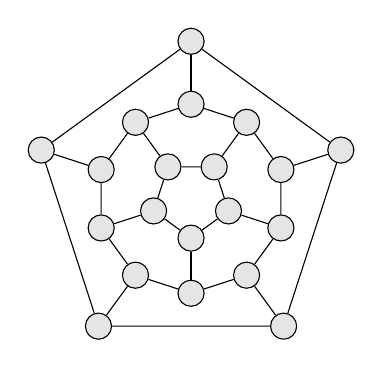
\begin{tikzpicture}
      \node[graph node, circle] (11) at (054:05mm) {}; 
      \node[graph node, circle] (13) at (126:05mm) {}; 
      \node[graph node, circle] (15) at (198:05mm) {}; 
      \node[graph node, circle] (17) at (270:05mm) {}; 
      \node[graph node, circle] (19) at (342:05mm) {}; 
      \node[graph node, circle] (20) at (018:12mm) {}; 
      \node[graph node, circle] (21) at (054:12mm) {}; 
      \node[graph node, circle] (22) at (090:12mm) {}; 
      \node[graph node, circle] (23) at (126:12mm) {}; 
      \node[graph node, circle] (24) at (162:12mm) {}; 
      \node[graph node, circle] (25) at (198:12mm) {}; 
      \node[graph node, circle] (26) at (234:12mm) {}; 
      \node[graph node, circle] (27) at (270:12mm) {}; 
      \node[graph node, circle] (28) at (306:12mm) {}; 
      \node[graph node, circle] (29) at (342:12mm) {}; 
      \node[graph node, circle] (30) at (018:20mm) {}; 
      \node[graph node, circle] (32) at (090:20mm) {}; 
      \node[graph node, circle] (34) at (162:20mm) {}; 
      \node[graph node, circle] (36) at (234:20mm) {}; 
      \node[graph node, circle] (38) at (306:20mm) {};

      \draw (11) -- (13) -- (15) -- (17) -- (19) -- (11);
      \draw (20) -- (21) -- (22) -- (23) -- (24) -- (25) -- (26) -- (27) -- (28) -- (29) -- (20);
      \draw (30) -- (32) -- (34) -- (36) -- (38) -- (30);

      \draw (20) -- (30);
      \draw (21) -- (11);
      \draw (22) -- (32);
      \draw (23) -- (13);
      \draw (24) -- (34);
      \draw (25) -- (15);
      \draw (26) -- (36);
      \draw (27) -- (17);
      \draw (28) -- (38);
      \draw (29) -- (19);
    \end{tikzpicture}
    \caption{Plateau de jeu pour le \emph{icosian game}}
    \label{figure:hamiltoncircuit:icosian}
  \end{subfigure}%
}

\newcommand\herschel{
  \begin{subfigure}{0.5\textwidth}
    \centering
    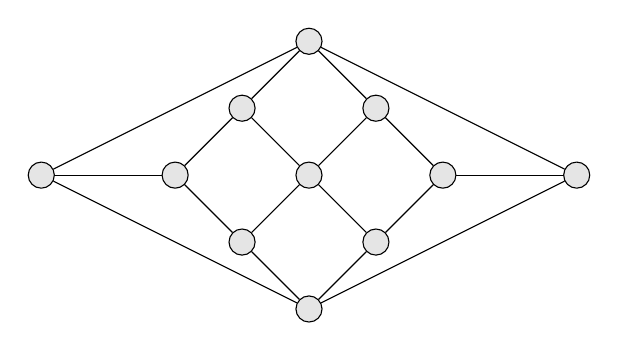
\begin{tikzpicture}[x=8.5mm, y=8.5mm]
      \node[graph node, circle] (44) at (4,4) {}; 
      \node[graph node, circle] (33) at (3,3) {}; 
      \node[graph node, circle] (53) at (5,3) {}; 
      \node[graph node, circle] (02) at (0,2) {}; 
      \node[graph node, circle] (22) at (2,2) {}; 
      \node[graph node, circle] (42) at (4,2) {}; 
      \node[graph node, circle] (62) at (6,2) {}; 
      \node[graph node, circle] (82) at (8,2) {}; 
      \node[graph node, circle] (31) at (3,1) {}; 
      \node[graph node, circle] (51) at (5,1) {}; 
      \node[graph node, circle] (40) at (4,0) {}; 

      \draw (22) -- (31) -- (40);
      \draw (33) -- (42) -- (51);
      \draw (44) -- (53) -- (62);

      \draw (22) -- (33) -- (44);
      \draw (31) -- (42) -- (53);
      \draw (40) -- (51) -- (62);
      
      \draw (02) -- (22);
      \draw (62) -- (82);
      \draw (02) -- (40) -- (82) -- (44) -- (02);
    \end{tikzpicture}
    \caption{Graphe de Herschel}
    \label{figure:hamiltoncircuit:herschel}
  \end{subfigure}
}

\newcommand\reduction{
  \begin{subfigure}{0.49\textwidth}
    \centering
    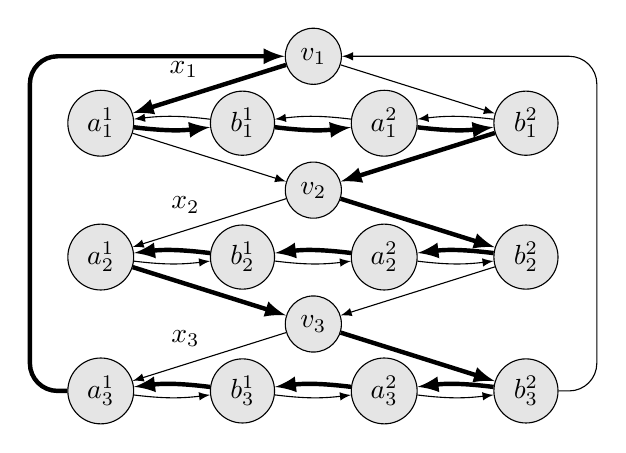
\begin{tikzpicture}[y=8.5mm, x=9mm]
      \coordinate (left)  at (1,0);
      \coordinate (right) at (9,0);

      \node[graph node, circle] (v1)  at (5,6) {$v_1$};
      \node[graph node, circle] (a11) at (2,5) {$a_1^1$};
      \node[graph node, circle] (b11) at (4,5) {$b_1^1$};
      \node[graph node, circle] (a12) at (6,5) {$a_1^2$};
      \node[graph node, circle] (b12) at (8,5) {$b_1^2$};
      \node[graph node, circle] (v2)  at (5,4) {$v_2$};
      \node[graph node, circle] (a21) at (2,3) {$a_2^1$};
      \node[graph node, circle] (b21) at (4,3) {$b_2^1$};
      \node[graph node, circle] (a22) at (6,3) {$a_2^2$};
      \node[graph node, circle] (b22) at (8,3) {$b_2^2$};
      \node[graph node, circle] (v3)  at (5,2) {$v_3$};
      \node[graph node, circle] (a31) at (2,1) {$a_3^1$};
      \node[graph node, circle] (b31) at (4,1) {$b_3^1$};
      \node[graph node, circle] (a32) at (6,1) {$a_3^2$};
      \node[graph node, circle] (b32) at (8,1) {$b_3^2$};
      
      \path[-latex, ultra thick] (v1) edge node[auto, swap]{$x_1$} (a11);
      \path[-latex            ] (v1) edge (b12);

      \path[-latex, ultra thick] (a11) edge[bend right=7] (b11);
      \path[-latex            ] (b11) edge[bend right=7] (a11);
      \path[-latex, ultra thick] (b11) edge[bend right=7] (a12);
      \path[-latex            ] (a12) edge[bend right=7] (b11);
      \path[-latex, ultra thick] (a12) edge[bend right=7] (b12);
      \path[-latex            ] (b12) edge[bend right=7] (a12);

      \path[-latex            ] (a11) edge (v2);
      \path[-latex, ultra thick] (b12) edge (v2);
      \path[-latex            ] (v2)  edge node[auto, swap]{$x_2$} (a21);
      \path[-latex, ultra thick] (v2)  edge (b22);

      \path[-latex            ] (a21) edge[bend right=7] (b21);
      \path[-latex, ultra thick] (b21) edge[bend right=7] (a21);
      \path[-latex            ] (b21) edge[bend right=7] (a22);
      \path[-latex, ultra thick] (a22) edge[bend right=7] (b21);
      \path[-latex            ] (a22) edge[bend right=7] (b22);
      \path[-latex, ultra thick] (b22) edge[bend right=7] (a22);

      \path[-latex, ultra thick] (a21) edge (v3);
      \path[-latex            ] (b22) edge (v3);
      \path[-latex            ] (v3)  edge node[auto, swap]{$x_3$} (a31);
      \path[-latex, ultra thick] (v3)  edge (b32);

      \path[-latex            ] (a31) edge[bend right=7] (b31);
      \path[-latex, ultra thick] (b31) edge[bend right=7] (a31);
      \path[-latex            ] (b31) edge[bend right=7] (a32);
      \path[-latex, ultra thick] (a32) edge[bend right=7] (b31);
      \path[-latex            ] (a32) edge[bend right=7] (b32);
      \path[-latex, ultra thick] (b32) edge[bend right=7] (a32);

      \draw[-latex, rounded corners=10, ultra thick] (a31) to (left |-a31) to (left |-v1) to (v1);
      \draw[-latex, rounded corners=10            ] (b32) to (right|-b32) to (right|-v1) to (v1);
    \end{tikzpicture}
    \caption{Structure de base de la réduction}
    \label{figure:hamiltoncircuit:reduction}
  \end{subfigure}%
}

\newcommand\gadget{
  \begin{subfigure}{0.49\textwidth}
    \centering
    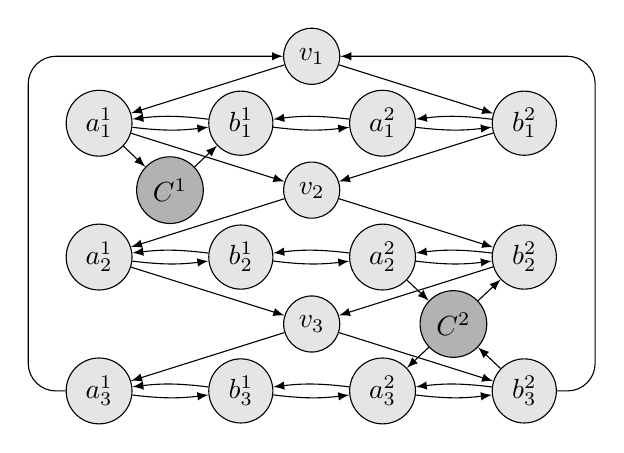
\begin{tikzpicture}[y=8.5mm, x=9mm]
      \coordinate (left)  at (1,0);
      \coordinate (right) at (9,0);

      \node[graph node, circle] (v1)  at (5,6) {$v_1$};
      \node[graph node, circle] (a11) at (2,5) {$a_1^1$};
      \node[graph node, circle] (b11) at (4,5) {$b_1^1$};
      \node[graph node, circle] (a12) at (6,5) {$a_1^2$};
      \node[graph node, circle] (b12) at (8,5) {$b_1^2$};
      \node[graph node, circle] (v2)  at (5,4) {$v_2$};
      \node[graph node, circle] (a21) at (2,3) {$a_2^1$};
      \node[graph node, circle] (b21) at (4,3) {$b_2^1$};
      \node[graph node, circle] (a22) at (6,3) {$a_2^2$};
      \node[graph node, circle] (b22) at (8,3) {$b_2^2$};
      \node[graph node, circle] (v3)  at (5,2) {$v_3$};
      \node[graph node, circle] (a31) at (2,1) {$a_3^1$};
      \node[graph node, circle] (b31) at (4,1) {$b_3^1$};
      \node[graph node, circle] (a32) at (6,1) {$a_3^2$};
      \node[graph node, circle] (b32) at (8,1) {$b_3^2$};

      \node[graph node, circle, fill=black!30] (C1)  at (3,4) {$C^1$};
      \node[graph node, circle, fill=black!30] (C2)  at (7,2) {$C^2$};
      
      \path[-latex] (v1) edge (a11);
      \path[-latex] (v1) edge (b12);

      \path[-latex] (a11) edge[bend right=7] (b11);
      \path[-latex] (b11) edge[bend right=7] (a11);
      \path[-latex] (b11) edge[bend right=7] (a12);
      \path[-latex] (a12) edge[bend right=7] (b11);
      \path[-latex] (a12) edge[bend right=7] (b12);
      \path[-latex] (b12) edge[bend right=7] (a12);

      \path[-latex] (a11) edge (v2);
      \path[-latex] (b12) edge (v2);
      \path[-latex] (v2)  edge (a21);
      \path[-latex] (v2)  edge (b22);

      \path[-latex] (a21) edge[bend right=7] (b21);
      \path[-latex] (b21) edge[bend right=7] (a21);
      \path[-latex] (b21) edge[bend right=7] (a22);
      \path[-latex] (a22) edge[bend right=7] (b21);
      \path[-latex] (a22) edge[bend right=7] (b22);
      \path[-latex] (b22) edge[bend right=7] (a22);

      \path[-latex] (a21) edge (v3);
      \path[-latex] (b22) edge (v3);
      \path[-latex] (v3)  edge (a31);
      \path[-latex] (v3)  edge (b32);

      \path[-latex] (a31) edge[bend right=7] (b31);
      \path[-latex] (b31) edge[bend right=7] (a31);
      \path[-latex] (b31) edge[bend right=7] (a32);
      \path[-latex] (a32) edge[bend right=7] (b31);
      \path[-latex] (a32) edge[bend right=7] (b32);
      \path[-latex] (b32) edge[bend right=7] (a32);

      \path[-latex] (a11) edge               (C1);  \path[-latex] (C1)  edge (b11);
      \path[-latex] (a22) edge               (C2);  \path[-latex] (C2)  edge (b22);
      \path[-latex] (b32) edge               (C2);  \path[-latex] (C2)  edge (a32);

      
      \draw[-latex, rounded corners=10] (a31) to (left |-a31) to (left |-v1) to (v1);
      \draw[-latex, rounded corners=10] (b32) to (right|-b32) to (right|-v1) to (v1);
    \end{tikzpicture}
    \caption{Instrumentation par gadgets (portes de clauses)}
    \label{figure:hamiltoncircuit:gadgets}
  \end{subfigure}%
}

\begin{exercice}[\textsc{Circuit Hamiltonien} est NP-complet%
    \footnote{Vidéo détaillée de la réduction de \textsc{3-SAT} à \textsc{Cycle Hamiltonien} : \url{https://www.youtube.com/watch?v=OHnX-R_SBpM}}]
  \label{exo:reductions/complexity/hamiltonian}

  On commence par introduire quelques définitions sur les graphes.
  \begin{itemize}
  \item Un \emph{graphe orienté} est un couple $G = \langle S, A \rangle$,
    où $S$ est l'ensemble de ses \emph{sommets}
    et $A \subseteq S \times S$ est l'ensemble de ses \emph{arcs}.
  \item Un \emph{chemin} de $G$ est une suite finie de sommets $(s_1, s_2, \dots, s_n)$
    tels que pour tout $1 \le i < n$, $\langle s_i, s_{i+1} \rangle \in A$.
  \item Un \emph{circuit} de $G$ est un chemin qui revient à son point de départ, c'est-à-dire tel que $s_1 = s_n$.
  \item Un circuit de $G$ est dit \emph{hamiltonien} s'il passe \emph{une et une seule fois} par chaque sommet de $G$,
    c'est-à-dire si pour tout $s\in S$, il existe un unique $i \in \{1, \dots, n-1\}$ tel que $s_i = s$.
  \item Un graphe $G$ est dit \emph{hamiltonien} s'il existe un \emph{circuit hamiltonien} dans $G$.
  \end{itemize}

  On considère maintenant le problème \textsc{Circuit Hamiltonien} défini ci-dessous.
  Le but de cet exercice est de montrer que \textsc{Circuit Hamiltonien} est NP-complet.

  \Probleme{Circuit Hamiltonien}{
    Un graphe orienté $G$.
  }{
    $G$ est-il hamiltonien ?
  }

  \begin{question}
  \item On considère les graphes des figures \ref{figure:hamiltoncircuit:icosian} et \ref{figure:hamiltoncircuit:herschel}.
    Ces deux graphes sont-ils hamiltoniens ?
    Justifier en donnant un circuit hamiltonien, ou en expliquant brièvement pourquoi il ne peut pas y en avoir.
  \end{question}

  \begin{figure}[h]%
    \centering
    \icosian%
    \herschel%
  \end{figure}

  \ifcorrection{\newpage}

  \begin{correction}
    Le graphe de la figure~\ref{figure:hamiltoncircuit:icosian} est hamiltonien. On a par exemple le circuit suivant.
    \begin{center}
      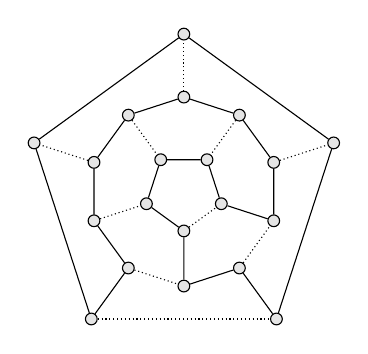
\begin{tikzpicture}
        \node[graph node, circle, inner sep=1.5pt] (11) at (054:05mm) {}; 
        \node[graph node, circle, inner sep=1.5pt] (13) at (126:05mm) {}; 
        \node[graph node, circle, inner sep=1.5pt] (15) at (198:05mm) {}; 
        \node[graph node, circle, inner sep=1.5pt] (17) at (270:05mm) {}; 
        \node[graph node, circle, inner sep=1.5pt] (19) at (342:05mm) {}; 
        \node[graph node, circle, inner sep=1.5pt] (20) at (018:12mm) {}; 
        \node[graph node, circle, inner sep=1.5pt] (21) at (054:12mm) {}; 
        \node[graph node, circle, inner sep=1.5pt] (22) at (090:12mm) {}; 
        \node[graph node, circle, inner sep=1.5pt] (23) at (126:12mm) {}; 
        \node[graph node, circle, inner sep=1.5pt] (24) at (162:12mm) {}; 
        \node[graph node, circle, inner sep=1.5pt] (25) at (198:12mm) {}; 
        \node[graph node, circle, inner sep=1.5pt] (26) at (234:12mm) {}; 
        \node[graph node, circle, inner sep=1.5pt] (27) at (270:12mm) {}; 
        \node[graph node, circle, inner sep=1.5pt] (28) at (306:12mm) {}; 
        \node[graph node, circle, inner sep=1.5pt] (29) at (342:12mm) {}; 
        \node[graph node, circle, inner sep=1.5pt] (30) at (018:20mm) {}; 
        \node[graph node, circle, inner sep=1.5pt] (32) at (090:20mm) {}; 
        \node[graph node, circle, inner sep=1.5pt] (34) at (162:20mm) {}; 
        \node[graph node, circle, inner sep=1.5pt] (36) at (234:20mm) {}; 
        \node[graph node, circle, inner sep=1.5pt] (38) at (306:20mm) {};

        \draw[densely dotted] (17) -- (19);
        \draw[densely dotted] (26) -- (27);
        \draw[densely dotted] (28) -- (29);
        \draw[densely dotted] (36) -- (38);

        \draw[densely dotted] (20) -- (30);
        \draw[densely dotted] (21) -- (11);
        \draw[densely dotted] (22) -- (32);
        \draw[densely dotted] (23) -- (13);
        \draw[densely dotted] (24) -- (34);
        \draw[densely dotted] (25) -- (15);
        
        \draw (38) -- (30) -- (32) -- (34) -- (36)
        -- (26) -- (25) -- (24) -- (23) -- (22) -- (21) -- (20) -- (29)
        -- (19) -- (11)-- (13) -- (15) -- (17)
        -- (27) -- (28)
        -- (38);
      \end{tikzpicture}
    \end{center}
    
    Le graphe de la figure~\ref{figure:hamiltoncircuit:herschel} n'est pas hamiltonien. Pour s'en convaincre, on peut tenter de construire un circuit hamiltonien,
    en choisissant un arc d'entrée et un arc de sortie pour le sommet central (en rouge), ce qui donne trois cas possibles,
    à symétrie près. Cela donne des contraintes sur les sommets adjacents (en bleu), puis sur les deux sommets extérieurs (en violet),
    et on arrive rapidement à une contradiction. 

    \begin{center}
      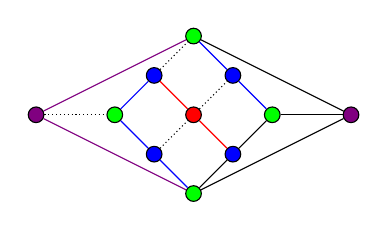
\begin{tikzpicture}[x=5mm, y=5mm]
        \node[graph node, circle, fill=green , inner sep=2pt] (44) at (4,4) {}; 
        \node[graph node, circle, fill=blue  , inner sep=2pt] (33) at (3,3) {}; 
        \node[graph node, circle, fill=blue  , inner sep=2pt] (53) at (5,3) {}; 
        \node[graph node, circle, fill=violet, inner sep=2pt] (02) at (0,2) {}; 
        \node[graph node, circle, fill=green , inner sep=2pt] (22) at (2,2) {}; 
        \node[graph node, circle, fill=red   , inner sep=2pt] (42) at (4,2) {}; 
        \node[graph node, circle, fill=green , inner sep=2pt] (62) at (6,2) {}; 
        \node[graph node, circle, fill=violet, inner sep=2pt] (82) at (8,2) {}; 
        \node[graph node, circle, fill=blue  , inner sep=2pt] (31) at (3,1) {}; 
        \node[graph node, circle, fill=blue  , inner sep=2pt] (51) at (5,1) {}; 
        \node[graph node, circle, fill=green , inner sep=2pt] (40) at (4,0) {}; 

        \draw[blue]           (22) to (31) to (40);
        \draw[red]            (33) to (42) to (51);
        \draw[blue]           (44) to (53) to (62);

        \draw[blue]           (22) to (33);
        \draw[densely dotted] (33) to (44);
        \draw[densely dotted] (31) to (42) to (53);
        \draw                 (40) to (51) to (62);
        
        \draw[densely dotted] (02) to (22);
        \draw                 (62) to (82);
        \draw[violet]         (44) to (02) to (40);
        \draw (40) to (82) to (44) ;
      \end{tikzpicture}
      \quad
      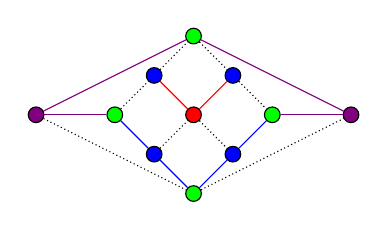
\begin{tikzpicture}[x=5mm, y=5mm]
        \node[graph node, circle, fill=green , inner sep=2pt] (44) at (4,4) {}; 
        \node[graph node, circle, fill=blue  , inner sep=2pt] (33) at (3,3) {}; 
        \node[graph node, circle, fill=blue  , inner sep=2pt] (53) at (5,3) {}; 
        \node[graph node, circle, fill=violet, inner sep=2pt] (02) at (0,2) {}; 
        \node[graph node, circle, fill=green , inner sep=2pt] (22) at (2,2) {}; 
        \node[graph node, circle, fill=red   , inner sep=2pt] (42) at (4,2) {}; 
        \node[graph node, circle, fill=green , inner sep=2pt] (62) at (6,2) {}; 
        \node[graph node, circle, fill=violet, inner sep=2pt] (82) at (8,2) {}; 
        \node[graph node, circle, fill=blue  , inner sep=2pt] (31) at (3,1) {}; 
        \node[graph node, circle, fill=blue  , inner sep=2pt] (51) at (5,1) {}; 
        \node[graph node, circle, fill=green , inner sep=2pt] (40) at (4,0) {}; 
        
        \draw[blue]           (22) to (31) to (40);
        \draw[red]            (33) to (42);
        \draw[densely dotted] (42) to (51);
        \draw[densely dotted] (44) to (53) to (62);
        
        \draw[densely dotted] (22) to (33) to (44);
        \draw[densely dotted] (31) to (42);
        \draw[red]            (42) to (53);
        \draw[blue]           (40) to (51) to (62);
        
        \draw[violet]         (02) to (22);
        \draw[violet]         (62) to (82);
        \draw[densely dotted] (02) to (40) to (82);
        \draw[violet]         (82) to (44) to (02);
      \end{tikzpicture}
      \quad
      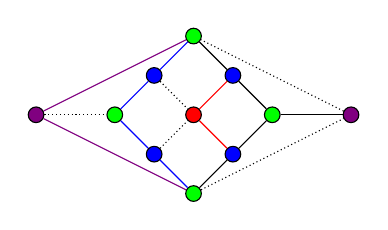
\begin{tikzpicture}[x=5mm, y=5mm]
        \node[graph node, circle, fill=green , inner sep=2pt] (44) at (4,4) {}; 
        \node[graph node, circle, fill=blue  , inner sep=2pt] (33) at (3,3) {}; 
        \node[graph node, circle, fill=blue  , inner sep=2pt] (53) at (5,3) {}; 
        \node[graph node, circle, fill=violet, inner sep=2pt] (02) at (0,2) {}; 
        \node[graph node, circle, fill=green , inner sep=2pt] (22) at (2,2) {}; 
        \node[graph node, circle, fill=red   , inner sep=2pt] (42) at (4,2) {}; 
        \node[graph node, circle, fill=green , inner sep=2pt] (62) at (6,2) {}; 
        \node[graph node, circle, fill=violet, inner sep=2pt] (82) at (8,2) {}; 
        \node[graph node, circle, fill=blue  , inner sep=2pt] (31) at (3,1) {}; 
        \node[graph node, circle, fill=blue  , inner sep=2pt] (51) at (5,1) {}; 
        \node[graph node, circle, fill=green , inner sep=2pt] (40) at (4,0) {}; 
        
        \draw[blue]           (22) to (31) to (40);
        \draw[densely dotted] (33) to (42);
        \draw[red]            (42) to (51);
        \draw                 (44) to (53) to (62);
        
        \draw[blue]           (22) to (33) to (44);
        \draw[densely dotted] (31) to (42);
        \draw[red]            (42) to (53);
        \draw                 (40) to (51) to (62);
        
        \draw[densely dotted] (02) to (22);
        \draw                 (62) to (82);
        \draw[violet]         (44) to (02) to (40);
        \draw[densely dotted] (40) to (82) to (44) ;
      \end{tikzpicture}
    \end{center}
  \end{correction}

  
  \begin{question}
  \item On cherche maintenant à montrer que \textsc{Circuit Hamiltonien} est dans NP.
    Quelle forme peut prendre un \emph{certificat} pour $G \in \textsc{Circuit Hamiltonien}$ ?
  \end{question}
  \begin{correction}
    Un certificat naturel est une \emph{liste ordonnée} $c = [c[1], c[2], \dots, c[n]]$ des sommets telle que le chemin
    $$(c[1], c[2], \dots, c[n], c[1])$$
    est un circuit hamiltonien de $G$. 
  \end{correction}

  \begin{question}
  \item Soit $G$ un graphe hamiltonien. Montrer que la \emph{taille} d'un tel certificat pour $G$
    est polynomiale par rapport à la taille de l'entrée $G$.
  \end{question}
  \begin{correction}
    En encodant un sommet par son identifiant, la taille du certificat est $n$ identifiants,
    donc $\mathcal{O}(n\log n)$ bits si les identifiants sont sur $\mathcal{O}(\log n)$ bits.
    Par rapport à une entrée encodée en listes d'adjacence (taille $\Theta(|S| + |A|)$)
    ou matrice d'adjacence (taille $\Theta(|S|^2)$), la taille du certificat est \emph{polynomiale}.
  \end{correction}

  \ifcorrection{\newpage}
  \begin{question}
  \item Proposer un \emph{algorithme vérificateur} qui, étant donné en entrée un graphe $G$ et un candidat $c$,
    décide si $c$ est un certificat \emph{valide} pour l'appartenance de $G$ à \textsc{Circuit Hamiltonien}.
  \end{question}
  \begin{correction}
    On a un algorithme simple en $\mathcal{O}(n^3)$. \\
    \begin{algorithm}[H]
      \SetKwFunction{Verify}{verify}
      \SetKwFunction{Contains}{contains}
      \SetKwFunction{Length}{length}
      \Fun{$\Verify(G=\langle S, A \rangle, c) $}{
        \tcp{vérification de $n = |S|$ en $\mathcal{O}(1)$}
        \lIf{$|c| \neq |S|$}{
          \Return \False;
        }
        \tcp{vérification que tous les sommets du chemin sont dans $G$ en $\mathcal{O}(n)$}
        \For{$i$ \From $1$ \To $n$}{
          \lIf{$\lnot \Contains(S, c[i])$}{
            \Return \False;
          }
        }
        
        \tcp{vérification de l'unicité des $c[i]$ en $\mathcal{O}(n^2)$}
        \For{$i$ \From $1$ \To $n$}{
          \For{$j$ \From $1$ \To $n$}{
            \lIf{$i \neq j \land c[i] = c[j]$}{
              \Return \False;
            }
          }
        }
        \tcp{vérification que les arcs sont bien présents en $\mathcal{O}(n \times m) = \mathcal{O}(n^3)$}
        \For{$i$ \From $1$ \To $n$}{
          \lIf{$\lnot \Contains(A, \langle c[i], c[i \mod n + 1] \rangle)$}{
            \Return \False;
          }
        }
        \Return \True;
      }
      \tcp{Cherche un élément dans un tableau en $\mathcal{O}(|tab|)$}
      \Fun{$\Contains(\mathit{tab}, \mathit{element}) $}{
        \For{$i$ \From $1$ \To $\mathit{tab}.\Length()$}{
          \lIf{$\mathit{tab}[i] = \mathit{element}$}{
            \Return \True;
          }
        }
        \Return \False;
      }
    \end{algorithm}
  \end{correction}

  \begin{question}
  \item Calculer la \emph{complexité en temps} dans le pire cas de votre vérificateur.
  \end{question}
  \begin{correction}
    On a un algorithme en $\mathcal{O}(n^3)$, où $n$ est inférieur à la taille des entrées (puisque $c$ est en $\mathcal{O}(n \log(n))$),
    donc en temps \emph{polynomial} en la taille de l'entrée.
  \end{correction}

  \begin{question}
  \item Conclure que \textsc{Circuit Hamiltonien} est dans NP.
  \end{question}
  \begin{correction}
    Il existe un certificat de taille polynomiale (une permutation des sommets) et un vérificateur en temps polynomial.  
    Par définition, $\textsc{Circuit Hamiltonien} \in \mathbf{NP}$.
  \end{correction}

  \ifnotcorrection{\pagebreak}
  On cherche maintenant à démontrer que le problème \textsc{Circuit Hamiltonien} est NP-dur par une réduction polynomiale de \textsc{Sat} vers \textsc{Circuit Hamiltonien}.
  On rappelle :

  \Probleme{Sat}{
    Une formule booléenne $\varphi$ en forme normale conjonctive (FNC), construite sur un ensemble $X=\{x_1,\dots,x_n\}$ de variables.
  }{
    Existe-t-il une affectation (Vrai/Faux) de chaque variable $x_i$ qui rend $\varphi$ satisfiable ?
  }

  On considère les circuits \emph{à rotation près} : par exemple $(1,2,3,1)$ et $(2,3,1,2)$ représentent le même circuit.

  \ifcorrection{\newpage}
  \begin{question}
  \item Dans le graphe de la figure~\ref{figure:hamiltoncircuit:reduction}, combien existe-t-il de circuits hamiltoniens (à rotation près) ? 
  \end{question}
  \begin{correction}
    Par rotation, on peut choisir de commencer par le sommet $v_1$. Le schéma impose, pour chaque $i\in\{1,2,3\}$,
    un choix binaire au sommet $v_i$ : emprunter l'arc $\langle v_i,a_i^1\rangle$ ou l'arc $\langle v_i, b_i^2\rangle$.  
    Ces choix sont indépendants et, pour chacun, il n'y a qu'une seule façon d'inclure tous les sommets $a_i^j$ et $b_i^j$. 
    \emph{À rotation près}, on obtient donc exactement $2^3=8$ circuits hamiltoniens,
    correspondant à tous les choix possibles de sortie des trois $v_i$.
  \end{correction}
  
  Pour $i \in \{1,2,3\}$, on note $x_i$ le prédicat unaire sur les circuits $c$ défini par :
  $x_i(c) \eqdef \text{$c$ emprunte l'arc}\langle v_i, a_i^1\rangle$.

  \begin{question}
  \item Caractériser de manière \emph{unique} le circuit hamiltonien $c_0$ dessiné en gras sur la figure~\ref{figure:hamiltoncircuit:reduction}
    par une formule booléenne en $x_1(c_0)$, $x_2(c_0)$ et $x_3(c_0)$.
  \end{question}

  \begin{figure}[h!]%
    \centering
    \reduction%
    \gadget%
  \end{figure}

  \begin{correction}
    Dans le circuit en gras, un choix est imposé pour chaque $x_i(c_0)$ :
    $x_1(c_0)=\text{Vrai}$, $x_2(c_0)=\text{Faux}$ et $x_3(c_0)=\text{Faux}$.
    C'est donc l'unique circuit hamiltonien \emph{à rotation près} du graphe tel que :
    $$ x_1 \land \lnot x_2 \land \lnot x_3.$$
  \end{correction}
  
  \begin{question}
  \item On ajoute un nouveau sommet $C^1$ et deux arcs $\langle a_1^1, C^1\rangle$ et $\langle C^1, b_1^1\rangle$
    comme à gauche de la figure~\ref{figure:hamiltoncircuit:gadgets}.
    Définir un prédicat logique $P(c)$ sur les circuits hamiltoniens $c$,
    exprimé en fonction de $x_1(c)$, $x_2(c)$ et $x_3(c)$,
    qui caractérise l'ensemble des circuits hamiltoniens du graphe \emph{modifié}. 
  \end{question}
  \begin{correction}
    Tout circuit hamiltonien doit désormais \emph{nécessairement} passer par $C^1$.
    Or $C^1$ n'est accessible que si le parcours a pris la branche gauche au niveau de $v_1$ (celle qui mène à $a_1^1$ puis vers $b_1^1$).  
    Par conséquent, l’ensemble des circuits hamiltoniens du graphe \emph{modifié} est exactement $\{c \mid P(c) \}$, où $P(c)  \eqdef x_1(c)$. 
  \end{correction}

  \begin{question}
  \item Caractériser tous les circuits hamiltoniens du graphe de la figure~\ref{figure:hamiltoncircuit:gadgets}. 
  \end{question}
  \begin{correction}
    On a deux gadgets ($C^1$ et $C^2$), donc le prédicat est une conjonction des deux clauses : 
    \begin{itemize}
    \item $C_1$ impose seulement $x_1(c)$ ;
    \item $C^2$ peut être accédé soit par le chemin $a_2^2 \to C^2 \to b_2^2$, soit par le chemin $b_3^2 \to C^2 \to a_3^2$,
      et impose donc la disjonction $x_2(c) \lor \lnot x_3(c)$. 
    \end{itemize}
    L'ensemble des chemins hamiltoniens de ce graphe est donc $\{ c \mid x_1(c) \land (x_2(c) \lor \lnot x_3(c))\}$.
  \end{correction}

  \ifcorrection{\newpage}
  \begin{question}
  \item En modifiant localement la figure~\ref{figure:hamiltoncircuit:reduction} sur le même principe,
    proposer des graphes dont l'ensemble des circuits hamiltoniens est exactement :
    \begin{center}
      $\{c \mid \lnot x_2(c)\}$ \quad\quad $\{c \mid x_1(c) \land \lnot x_2(c)\}$  \quad\quad $\{c \mid x_1(c) \lor \lnot x_2(c)\}$ 
    \end{center}
  \end{question}
  \begin{correction}
    \begin{itemize}
    \item $\{ c \mid \lnot x_2(c) \}$ : insérer un sommet $C^2$ et deux arcs $\langle b_2^2, C^2\rangle$ et $\langle C^2, a_2^2 \rangle$
      ($C_2$ est entre $b_2^2$ et $a_2^2$, accessible de la droite vers la gauche)
    \item $\{ c \mid x_1(c) \land \lnot x_2(c) \}$ : combiner les deux portes précédentes
      (un sommet $C^1$ entre $a_1^1$ et $b_1^1$ et un sommet $C^2$ entre $b_2^2$ et $a_2^2$). 
    \item $\{ c \mid x_1(c) \lor \lnot x_2(c) \}$ : il faut utiliser le même sommet dans les deux portes.
      On ajoute un sommet $C$ et quatre arcs : $\langle a_1^1, C\rangle$, $\langle C, b_1^1 \rangle$, $\langle b_2^2, C\rangle$ et $\langle C, a_2^2 \rangle$.
    \end{itemize}
  \end{correction}
  
  \begin{question}
  \item Construire un graphe orienté dont les circuits hamiltoniens sont exactement les circuits $c$ tels que :
    $$(\lnot x_1(c) \lor \lnot x_2(c) \lor x_4(c)) \land (x_1(c) \lor x_2(c)) \land (\lnot x_2(c) \lor x_3(c) \lor \lnot x_4(c))$$
  \end{question}
  \begin{correction}
    Attention, la formule $\varphi$ a trois clauses et quatre variables, donc il faut agrandir le graphe de base pour avoir
    quatre gadgets de variables contenant chacun trois sommets $a_i^j$ et trois sommets $b_i^j$. Voir le graphe sur la page suivante.

    \vspace{-2mm}
    \begin{center}
      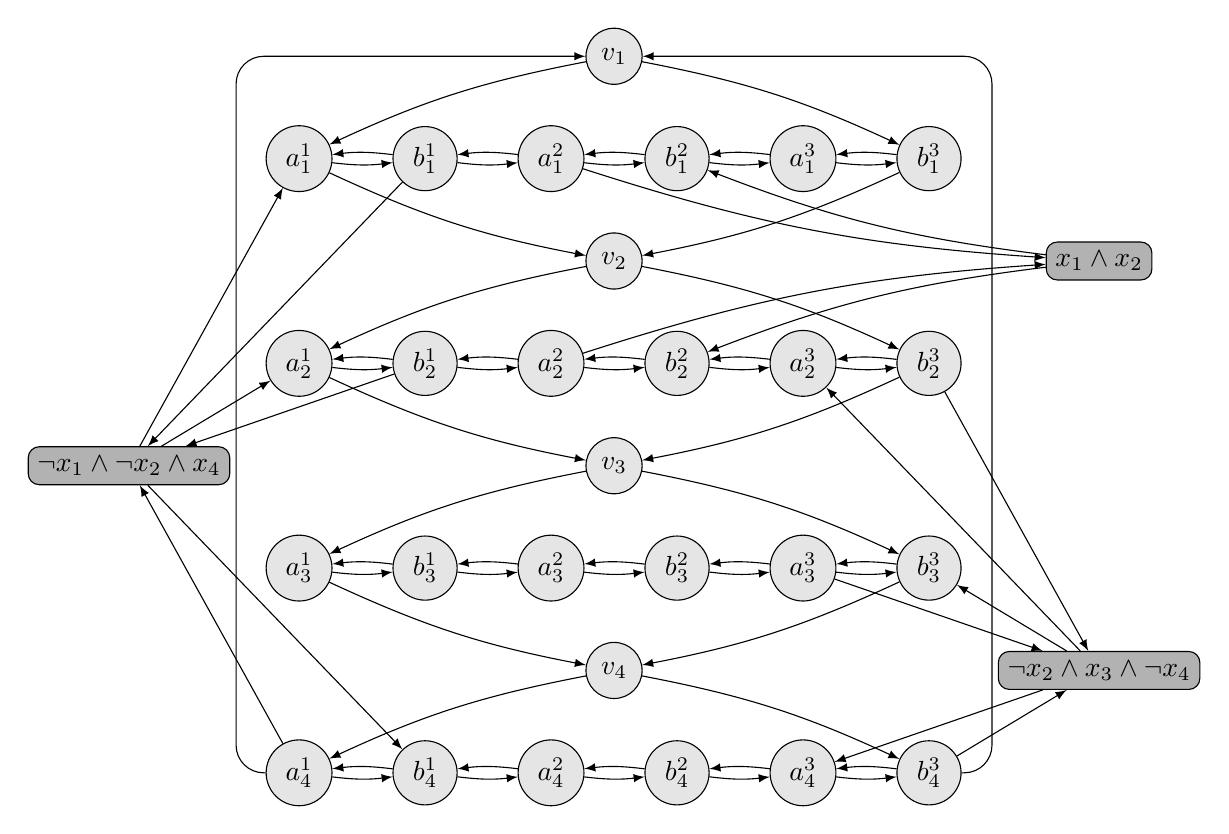
\begin{tikzpicture}[y=13mm, x=8mm]
        \coordinate (left)  at ( 1,0);
        \coordinate (right) at (13,0);

        \node[graph node, circle] (v1)  at ( 7,8) {$v_1$};
        \node[graph node, circle] (a11) at ( 2,7) {$a_1^1$};
        \node[graph node, circle] (b11) at ( 4,7) {$b_1^1$};
        \node[graph node, circle] (a12) at ( 6,7) {$a_1^2$};
        \node[graph node, circle] (b12) at ( 8,7) {$b_1^2$};
        \node[graph node, circle] (a13) at (10,7) {$a_1^3$};
        \node[graph node, circle] (b13) at (12,7) {$b_1^3$};
        \node[graph node, circle] (v2)  at ( 7,6) {$v_2$};
        \node[graph node, circle] (a21) at ( 2,5) {$a_2^1$};
        \node[graph node, circle] (b21) at ( 4,5) {$b_2^1$};
        \node[graph node, circle] (a22) at ( 6,5) {$a_2^2$};
        \node[graph node, circle] (b22) at ( 8,5) {$b_2^2$};
        \node[graph node, circle] (a23) at (10,5) {$a_2^3$};
        \node[graph node, circle] (b23) at (12,5) {$b_2^3$};
        \node[graph node, circle] (v3)  at ( 7,4) {$v_3$};
        \node[graph node, circle] (a31) at ( 2,3) {$a_3^1$};
        \node[graph node, circle] (b31) at ( 4,3) {$b_3^1$};
        \node[graph node, circle] (a32) at ( 6,3) {$a_3^2$};
        \node[graph node, circle] (b32) at ( 8,3) {$b_3^2$};
        \node[graph node, circle] (a33) at (10,3) {$a_3^3$};
        \node[graph node, circle] (b33) at (12,3) {$b_3^3$};
        \node[graph node, circle] (v4)  at ( 7,2) {$v_4$};
        \node[graph node, circle] (a41) at ( 2,1) {$a_4^1$};
        \node[graph node, circle] (b41) at ( 4,1) {$b_4^1$};
        \node[graph node, circle] (a42) at ( 6,1) {$a_4^2$};
        \node[graph node, circle] (b42) at ( 8,1) {$b_4^2$};
        \node[graph node, circle] (a43) at (10,1) {$a_4^3$};
        \node[graph node, circle] (b43) at (12,1) {$b_4^3$};

        \node[graph node, fill=black!30] (C1) at ( -.7,4) {$\lnot x_1 \land \lnot x_2 \land x_4$};
        \path[-latex] (b11) edge (C1);
        \path[-latex] (C1)  edge (a11);
        \path[-latex] (b21) edge (C1);
        \path[-latex] (C1)  edge (a21);
        \path[-latex] (a41) edge (C1);
        \path[-latex] (C1)  edge (b41);

        \node[graph node, fill=black!30] (C2) at (14.7,6) {$x_1 \land x_2$};
        \path[-latex] (a12) edge[bend right=7] (C2);
        \path[-latex] (C2)  edge[bend left=7 ] (b12);
        \path[-latex] (a22) edge[bend left=7 ] (C2);
        \path[-latex] (C2)  edge[bend right=7] (b22);

        \node[graph node, fill=black!30] (C3) at (14.7,2) {$\lnot x_2 \land x_3 \land \lnot x_4$};
        \path[-latex] (b23) edge (C3);
        \path[-latex] (C3)  edge (a23);
        \path[-latex] (a33) edge (C3);
        \path[-latex] (C3)  edge (b33);
        \path[-latex] (b43) edge (C3);
        \path[-latex] (C3)  edge (a43);
        
        \path[-latex] (v1) edge[bend right=7] (a11);
        \path[-latex] (v1) edge[bend left =7] (b13);

        \path[-latex] (a11) edge[bend right=7] (b11);
        \path[-latex] (b11) edge[bend right=7] (a11);
        \path[-latex] (b11) edge[bend right=7] (a12);
        \path[-latex] (a12) edge[bend right=7] (b11);
        \path[-latex] (a12) edge[bend right=7] (b12);
        \path[-latex] (b12) edge[bend right=7] (a12);
        \path[-latex] (b12) edge[bend right=7] (a13);
        \path[-latex] (a13) edge[bend right=7] (b12);
        \path[-latex] (a13) edge[bend right=7] (b13);
        \path[-latex] (b13) edge[bend right=7] (a13);

        \path[-latex] (a11) edge[bend right=7] (v2);
        \path[-latex] (b13) edge[bend left =7] (v2);
        \path[-latex] (v2)  edge[bend right=7] (a21);
        \path[-latex] (v2)  edge[bend left =7] (b23);

        \path[-latex] (a21) edge[bend right=7] (b21);
        \path[-latex] (b21) edge[bend right=7] (a21);
        \path[-latex] (b21) edge[bend right=7] (a22);
        \path[-latex] (a22) edge[bend right=7] (b21);
        \path[-latex] (a22) edge[bend right=7] (b22);
        \path[-latex] (b22) edge[bend right=7] (a22);
        \path[-latex] (b22) edge[bend right=7] (a23);
        \path[-latex] (a23) edge[bend right=7] (b22);
        \path[-latex] (a23) edge[bend right=7] (b23);
        \path[-latex] (b23) edge[bend right=7] (a23);

        \path[-latex] (a21) edge[bend right=7] (v3);
        \path[-latex] (b23) edge[bend left =7] (v3);
        \path[-latex] (v3)  edge[bend right=7] (a31);
        \path[-latex] (v3)  edge[bend left =7] (b33);

        \path[-latex] (a31) edge[bend right=7] (b31);
        \path[-latex] (b31) edge[bend right=7] (a31);
        \path[-latex] (b31) edge[bend right=7] (a32);
        \path[-latex] (a32) edge[bend right=7] (b31);
        \path[-latex] (a32) edge[bend right=7] (b32);
        \path[-latex] (b32) edge[bend right=7] (a32);
        \path[-latex] (b32) edge[bend right=7] (a33);
        \path[-latex] (a33) edge[bend right=7] (b32);
        \path[-latex] (a33) edge[bend right=7] (b33);
        \path[-latex] (b33) edge[bend right=7] (a33);

        \path[-latex] (a31) edge[bend right=7] (v4);
        \path[-latex] (b33) edge[bend left =7] (v4);
        \path[-latex] (v4)  edge[bend right=7] (a41);
        \path[-latex] (v4)  edge[bend left =7] (b43);

        \path[-latex] (a41) edge[bend right=7] (b41);
        \path[-latex] (b41) edge[bend right=7] (a41);
        \path[-latex] (b41) edge[bend right=7] (a42);
        \path[-latex] (a42) edge[bend right=7] (b41);
        \path[-latex] (a42) edge[bend right=7] (b42);
        \path[-latex] (b42) edge[bend right=7] (a42);
        \path[-latex] (b42) edge[bend right=7] (a43);
        \path[-latex] (a43) edge[bend right=7] (b42);
        \path[-latex] (a43) edge[bend right=7] (b43);
        \path[-latex] (b43) edge[bend right=7] (a43);
        
        \draw[-latex, rounded corners=10] (a41) to (left |-a41) to (left |-v1) to (v1);
        \draw[-latex, rounded corners=10] (b43) to (right|-b43) to (right|-v1) to (v1);
      \end{tikzpicture}
    \end{center}
  \end{correction}
  
  \ifcorrection{\newpage}
  \begin{question}
  \item Définir une transformation $\mathcal{G}$ qui, à toute formule $\varphi$
    en forme normale conjonctive sur des variables $x_1,\dots,x_n$, associe un graphe orienté $\mathcal{G}(\varphi)$
    dont $\varphi$ caractérise les circuits hamiltoniens.
    En déduire que $\varphi \in \textsc{Sat} \iff \mathcal{G}(\varphi) \in \textsc{Circuit Hamiltonien}$.
  \end{question}
  \begin{correction}
    $$
    \begin{array}{rcl@{\quad}l}
      \mathcal{G}(\varphi) &=& \langle S(\varphi), A(\varphi) \rangle, \text{ avec :} \\
      S(\varphi) &=&  \{ v_i   \mid 1 \le i \le n  \}                                                                                                     & \le n\\
      &\cup& \{ a_i^j \mid 1 \le i \le n \land 1 \le j \le k\}                                                                                            & \le n \times k\\
      &\cup& \{ b_i^j \mid 1 \le i \le n \land 1 \le j \le k\}                                                                                            & \le n \times k\\
      &\cup& \{ C^j   \mid 1 \le j \le k\}                                                                                                                 & \le k\\ 
      A(\varphi) &=&  \{ \langle v_i, a_i^1 \rangle, \langle v_i, b_i^k  \rangle             \mid 1 \le i \le n  \}                                        & \le n\\
      &\cup& \{ \langle a_i^1, v_{i \bmod n + 1} \rangle, \langle b_i^k, v_{i \bmod n + 1} \rangle \mid 1 \le i \le n  \}                                        & \le n\\
      &\cup& \{ \langle a_i^j, b_i^j \rangle,          \langle b_i^j, a_i^j \rangle          \mid 1 \le i \le n  \land 1 \le j \le k \}                    & \le n \times k\\
      &\cup& \{ \langle b_i^j, a_i^{j+1} \rangle,       \langle a_i^{j+1}, b_i^j \rangle       \mid 1 \le i \le n  \land 1 \le j < k \}                      & \le n \times k\\
      &\cup& \{ \langle a_i^j, C^j \rangle,            \langle C^j, b_i^j \rangle            \mid x_i \text{ est un litéral de la clause } C^j \}          & \le n \times k\\
      &\cup& \{ \langle b_i^j, C^j \rangle,            \langle C^j, a_i^j \rangle            \mid \lnot x_i \text{ est un litéral de la clause } C^j \}    & \le n \times k
    \end{array}
    $$
    La formule $\varphi$ décrit précisément les circuits hamiltoniens de $\mathcal{G}(\varphi)$.
    Il existe donc une affectation des variables de $\varphi$ si, et seulement si,
    il existe un circuits hamiltoniens dans $\mathcal{G}(\varphi)$.
    Autrement dit, $$\varphi \in \textsc{Sat} \iff \mathcal{G}(\varphi) \in \textsc{Circuit Hamiltonien}.$$
  \end{correction}
  
  \begin{question}
  \item Soit $\varphi$ une formule à $n$ variables, et $k$ clauses.
    \begin{itemize}
    \item donner une surapproximation du nombre de sommets et d'arcs de $\mathcal{G}(\varphi)$ en fonction de $n$ et $k$ ;
    \item conclure que la construction $\mathcal{G}$ s'effectue en temps polynomial.
    \end{itemize}
  \end{question}
  \begin{correction}
    Le calcul est détaillé sur la transformation de la question précédente.
    Le nombre de sommets dans $\mathcal{G}(\varphi)$ est borné par $2 n k + n + k = \mathcal{O}(n k)$.
    Le nombre d'arcs dans $\mathcal{G}(\varphi)$ est borné par $4 n k + 2 n = \mathcal{O}(n k)$.
    La transformation n'a pas de difficulté algorithmique, donc elle s'effectue en temps polynomial.
  \end{correction}
  
  \begin{question}
  \item Que peut-on conclure sur la complexité de \textsc{Circuit Hamiltonien} ? 
  \end{question}
  \begin{correction}
    On a une réduction polynomiale de \textsc{Sat} vers \textsc{Circuit Hamiltonien}.
    On en déduit que \textsc{Circuit Hamiltonien} est NP-difficile.
    De plus, on sait que \textsc{Circuit Hamiltonien} est NP.
    On en déduit que \textsc{Circuit Hamiltonien} est NP-complet.
  \end{correction}

\end{exercice}

\endgroup
\endinput

 
 
\session{Ensembles stables d'un graphe}
% SPDX-License-Identifier: CC-BY-SA-4.0
% Author: Matthieu Perrin
% Part: Introduction
% Section: Words and languages
% Exercise: Words

\begingroup

\begin{exercice}[Le problème \textsc{Ensemble Stable}]

  Étant donné un graphe $G$, un {\em ensemble stable} de $G$ est un ensemble de sommets deux à deux non adjacents dans $G$.
  Autrement dit, pour toute paire $u, v$ de sommets de cet ensemble, l'arête $\langle u, v\rangle$ {\em n'existe pas} dans $G$.

  Par exemple, dans le graphe ci-dessous, les sommets $1, 4, 5$ et $6$ forment un ensemble stable.

  \begin{center}
    \begin{tikzpicture}[x=10mm, y=10mm]
      \node[graph node, circle] (1) at (1,2) {1};
      \node[graph node, circle] (2) at (3,2) {2};
      \node[graph node, circle] (3) at (0,1) {3};
      \node[graph node, circle] (4) at (2,1) {4};
      \node[graph node, circle] (5) at (4,1) {5};
      \node[graph node, circle] (6) at (1,0) {6};
      \node[graph node, circle] (7) at (3,0) {7};

      \draw[thick] (3) -- (1) -- (2) -- (5) -- (7) -- (6) -- (3);
      \draw[thick] (3) -- (2) -- (4) -- (7) -- (3);
    \end{tikzpicture}
  \end{center}

  On s'intéresse au problème de décision \textsc{Ensemble Stable}:

  \Probleme{Ensemble Stable}{
    Une paire $\langle G, k \rangle$ formée d'un graphe non orienté $G=\langle V, E\rangle$ et d'un entier $k$.
  }{
    Existe-t-il un ensemble stable de taille au moins $k$ dans $G$ ?
  }

  Le but de cet exercice est de montrer qu'\textsc{Ensemble Stable} est NP-complet.
  
  \begin{question}
  \item\label{ex3.Q8} Expliquez pourquoi le problème \textsc{Ensemble Stable} appartient à la classe NP.
    Pour cela, précisez quel certificat fournir pour une réponse ``oui'', et expliquez comment vérifier ce certificat en temps polynomial.
  \end{question}
  \begin{correction}
    Un certificat pour le problème \textsc{Ensemble Stable} est un tableau $T$ de $k$ sommets. Si l'instance est positive, on a forcément $k \le |E| \le |G|$.
    
    Pour vérifier ce certificat (qu'on suppose déjà parsé sous la forme d'un tableau), il faut
    \begin{itemize}
    \item vérifier que la longueur est bien $k$, en $\mathcal{O}(1)$; 
    \item vérifier que tous les éléments du tableau sont bien des éléments de $E$, en $\mathcal{O}(k)$; 
    \item pour chaque paire d'indices $0 \le i, j < k$, vérifier que $T[i] \neq T[j]$ et que $\langle i, j \rangle \notin E$.
      Il y a $\mathcal{O}(k^2)$ paires d'indices, et suivant l'encodage du graphe, chaque tour de boucle peut coûter jusqu'à  $\mathcal{O}(|G|)$. 
    \end{itemize}
    Finalement, vérifier le certificat est bien polynômial en la taille du graphe. 
  \end{correction}

  On souhaite maintenant démontrer que $\textsc{3-SAT} \leq_P \textsc{Ensemble Stable}$. On rappelle et précise la définition de \textsc{3-SAT}
  utilisée dans cet exercice. 

  \Probleme{3-SAT}{
    Une formule booléenne $\varphi = C_1 \wedge C_2 \wedge \ldots \wedge C_p$,  
    où chaque clause $C_i$ ($1 \leq i \leq p$) est une disjonction d'\textbf{exactement} trois littéraux,
    et chaque littéral est soit une variable $x_j$, soit une négation $\lnot x_j$  
    pour une variable $x_j$ parmi un ensemble $\{x_1, x_2, \ldots, x_n\}$.
  }{
    Existe-t-il une valuation $\{x_1, x_2, \ldots, x_n\} \rightarrow \{\text{vrai}, \text{faux}\}$ qui satisfait $\varphi$ ?
  }

  Pour les premières questions de l'exercice, on considère l'instance $\psi$ particulière de \textsc{3-SAT} suivante : 
  $$\psi =
  \underbrace{(x_1 \vee x_2 \vee \neg x_3)}_{C_1}
  \wedge
  \underbrace{(\neg x_1 \vee \neg x_2 \vee \neg x_4)}_{C_2}
  \wedge
  \underbrace{(\neg x_2 \vee x_3 \vee \neg x_4)}_{C_3}
  \wedge
  \underbrace{(\neg x_1 \vee \neg x_2 \vee x_4)}_{C_4}
  $$
  
  \ifcorrection{\newpage}
  \begin{question}
  \item\label{ex3.Q1} Déterminez des valeurs pour les variables $x_1, x_2, x_3$ et $x_4$ qui satisfont $\psi$.
  \end{question}
  \begin{correction}
    Par exemple, $x_1 = x_3 = \text{vrai}$ et $x_2 = x_4 = \text{faux}$
  \end{correction}
  
  On définit maintenant une transformation $f$ qui, à chaque formule $\varphi$ de \textsc{3-SAT},
  associe une instance \linebreak $f(\varphi) = \langle G, k\rangle$ du problème \textsc{Ensemble Stable} construite selon les règles suivantes :
  \begin{itemize}
  \item $k=p$ (le nombre de clauses de $\varphi$),
  \item le graphe $G$ est construit comme ceci.
    \begin{itemize}
    \item Pour chaque clause $C_i$, on ajoute un triangle dont chacun des 3 sommets aura pour nom ``$i:l$''
      formé de l'indice $i$ de la clause et d'un des littéraux $l$ de $C_i$.
      On appellera chaque triangle un ``\underline{triangle-clause}''.

      Par exemple, pour une clause $C_i=(x_2\vee \neg x_4 \vee x_5)$, on ajoute dans $G$:

      \begin{center}
        \begin{tikzpicture}[x=20mm, y=20mm]
          \node[graph node] (C) at (.5,0.866) {$i : x_2$};
          \node[graph node] (A) at (0,0) {$i : \lnot x_4$};
          \node[graph node] (B) at (1,0) {$i : x_5$};

          \draw[thick] (A) -- (B) -- (C) -- (A);
        \end{tikzpicture}
      \end{center}

    \item On relie chaque paire de sommets représentant des littéraux opposés ($i : x_m$ et $j : \neg x_m$) par une arête.

      Par exemple, pour deux clauses $C_i=(x_2\vee \neg x_4 \vee x_5)$ et $C_j=(\neg x_2\vee \neg x_4 \vee \neg x_5)$ de $\varphi$, on a la configuration suivante dans $G$:

      \begin{center}
        \begin{tikzpicture}[x=20mm, y=20mm]
          % Triangle i
          \node[graph node] (C) at (.5,0.866) {$i : x_2$};
          \node[graph node] (A) at (0,0)      {$i : \lnot x_4$};
          \node[graph node] (B) at (1,0)      {$i : x_5$};

          \draw[thick] (A) -- (B) -- (C) -- (A);

          % Triangle j
          \node[graph node] (F) at (3.5,0.866) {$j : \lnot x_2$};
          \node[graph node] (D) at (3,0)       {$j : \lnot x_4$};
          \node[graph node] (E) at (4,0)       {$j : \lnot x_5$};

          \draw[thick] (D) -- (E) -- (F) -- (D);

          % Liens inter-triangles
          \draw[blue, thick] (C) -- (F);
          \draw[red, thick] (B) to[bend right=20] (E);
        \end{tikzpicture}
      \end{center}

      
    \end{itemize}
  \end{itemize}
  
  \begin{question}
  \item\label{ex3.Q2} Fournissez l'instance $f(\psi) = \langle G_\psi, k_\psi \rangle$ d'\textsc{Ensemble Stable}
    obtenue par la transformation de la formule $\psi$ utilisée dans la question~\ref{ex3.Q1} : pour cela, dessinez $G_\psi$ et donnez la valeur de $k_\psi$.
  \end{question}
  \begin{correction}

    $k=4$
    
    \begin{tikzpicture}[xscale=2,yscale=2]

      % Clause C1 : (x1 ∨ x2 ∨ ¬x3)
      \node[circle, fill, inner sep=0pt, minimum size=4pt, label=above:$1 : x_2$] (C1C) at (1,1.7) {};
      \node[circle, fill, inner sep=0pt, minimum size=4pt, label=left:$1 : x_1$] (C1A) at (0.7,1.3) {};
      \node[circle, fill, inner sep=0pt, minimum size=4pt, label=right:$1 : \lnot x_3$] (C1B) at (1.3,1.3) {};
      \draw[thick] (C1A) -- (C1B) -- (C1C) -- (C1A);

      % Clause C2 : (¬x1 ∨ ¬x2 ∨ ¬x4)
      \node[circle, fill, inner sep=0pt, minimum size=4pt, label=above:$2 : \lnot x_2$] (C2C) at (3,1.7) {};
      \node[circle, fill, inner sep=0pt, minimum size=4pt, label=left:$2 : \lnot x_1$] (C2A) at (2.7,1.3) {};
      \node[circle, fill, inner sep=0pt, minimum size=4pt, label=right:$2 : \lnot x_4$] (C2B) at (3.3,1.3) {};
      \draw[thick] (C2A) -- (C2B) -- (C2C) -- (C2A);

      % Clause C3 : (¬x2 ∨ x3 ∨ ¬x4)
      \node[circle, fill, inner sep=0pt, minimum size=4pt, label=above:$3 : x_3$] (C3C) at (1,0.7) {};
      \node[circle, fill, inner sep=0pt, minimum size=4pt, label=left:$3 : \lnot x_2$] (C3A) at (0.7,0.3) {};
      \node[circle, fill, inner sep=0pt, minimum size=4pt, label=right:$3 : \lnot x_4$] (C3B) at (1.3,0.3) {};
      \draw[thick] (C3A) -- (C3B) -- (C3C) -- (C3A);

      % Clause C4 : (¬x1 ∨ ¬x2 ∨ x4)
      \node[circle, fill, inner sep=0pt, minimum size=4pt, label=above:$4 : x_4$] (C4C) at (3,0.7) {};
      \node[circle, fill, inner sep=0pt, minimum size=4pt, label=left:$4 : \lnot x_1$] (C4A) at (2.7,0.3) {};
      \node[circle, fill, inner sep=0pt, minimum size=4pt, label=right:$4 : \lnot x_2$] (C4B) at (3.3,0.3) {};
      \draw[thick] (C4A) -- (C4B) -- (C4C) -- (C4A);

      % Liaisons entre littéraux opposés
      \draw[red, thick] (C1A) to[out=-30,in=-150] (C2A); % x1 -- ¬x1
      \draw[red, thick] (C1A) -- (C4A); % x1 -- ¬x1
      \draw[red, thick] (C1C) -- (C2C); % x2 -- ¬x2
      \draw[red, thick] (C1C) -- (C3A); % x2 -- ¬x2
      \draw[red, thick] (C1C) -- (C4B); % x2 -- ¬x2
      \draw[red, thick] (C3C) -- (C1B); % x3 -- ¬x3
      \draw[red, thick] (C3B) -- (C4C); % ¬x4 -- x4
      \draw[red, thick] (C2B) -- (C4C); % ¬x4 -- x4
    \end{tikzpicture}
  \end{correction}

  \begin{question}
  \item\label{ex3.Q3} En vous appuyant sur la valuation trouvée à la question~\ref{ex3.Q1}
    et l'instance $\langle G_\psi, k_\psi \rangle$ obtenue dans la question~\ref{ex3.Q2},
    déterminez un ensemble stable de taille $k_\psi$ dans $G_\psi$.
  \end{question}
  \begin{correction}
    $\{ 1:x_1, 2:\lnot x_2, 3:\lnot x_2, 4:\lnot x_2\}$
  \end{correction}

  \ifcorrection{\newpage}
  On se place dans le cas général : on part d'une formule arbitraire $\varphi$ de \textsc{3-SAT}, et on considère l'instance 
  $f(\varphi) = \langle G, k\rangle$ du problème \textsc{Ensemble Stable}, construite comme précédemment.

  \begin{question}
  \item\label{ex3.Q4} En généralisant le raisonnement de la question~\ref{ex3.Q3},
    expliquez comment une valuation qui satisfait~$\varphi$ permet de construire
    un ensemble stable de taille~$k$ dans le graphe~$G$.
  \end{question}
  \begin{correction}
    Soit $v$ une valuation qui satisfait la formule $\varphi$. Par définition, chaque clause $C_i$ contient au moins un littéral $l_i$ tel que $l_i$ est satisfait par $v$.

    Pour chaque clause $C_i$, on choisit un tel littéral $l_i$ et on considère le sommet $i : l_i$ du triangle-clause correspondant dans le graphe $G$. On définit alors :
    $S = \{\, i : l_i \mid 1 \leq i \leq p \,\}$.

    Cet ensemble $S$ contient exactement un sommet par triangle-clause, donc $|S| = p = k$.

    Montrons que $S$ est un ensemble stable. Soient $i : l_i$ et $j : l_j$ deux sommets distincts de $S$.
    \begin{itemize}
    \item Comme $i \neq j$, ces sommets proviennent de deux triangles-clauses différents, donc ne sont pas adjacents par construction interne des triangles.
    \item De plus, les littéraux $l_i$ et $l_j$ ne peuvent pas être des littéraux opposés (c'est-à-dire de la forme $x$ et $\lnot x$), car une même valuation $v$ ne peut pas satisfaire à la fois une variable et sa négation.
    \end{itemize}

    Ainsi, aucun sommet de $S$ n’est adjacent à un autre, ce qui prouve que $S$ est un ensemble stable de taille $k$ dans le graphe $G$.
  \end{correction}

  \begin{question}
  \item\label{ex3.Q5} On suppose que $G$ admet un ensemble stable de taille $k$, que l'on note $V'$.
    Expliquez pourquoi $V'$ contient {\em exactement un} sommet dans chaque triangle-clause, et
    pourquoi $V'$ ne peut pas contenir deux sommets correspondant à des littéraux opposés (de la forme $x_j$ et $\neg x_j$).
  \end{question}
  \begin{correction}
    \begin{itemize}
    \item Chaque triangle-clause ajouté dans la construction de $G$ correspond à une clause $C_i$ de la formule $\varphi$, et contient exactement 3 sommets, reliés entre eux. Par définition d’un ensemble stable, $V'$ ne peut contenir plus d’un sommet par triangle-clause. Or, il y a $p$ clauses, donc $p$ triangles, et $|V'| = p$ ; par conséquent, $V'$ contient exactement un sommet dans chaque triangle-clause.

    \item Soient $i : l$ et $j : l'$ deux sommets distincts de $V'$. Comme $V'$ est un ensemble stable, les sommets $i : l$ et $j : l'$ ne sont pas adjacents. Or, dans le graphe $G$, les seules arêtes entre triangles-clause relient des sommets correspondant à des littéraux opposés (de la forme $x$ et $\lnot x$). Il s’ensuit que $l$ et $l'$ ne peuvent pas être des littéraux opposés. Autrement dit, $V'$ ne contient pas deux littéraux contradictoires.
    \end{itemize}
  \end{correction}

  \begin{question}
  \item Déduisez-en comment construire une valuation des variables qui satisfait $\varphi$ à partir des sommets de $V'$.
    Justifiez pourquoi cette méthode fonctionne.
  \end{question}
  \begin{correction}
    On peut alors définir une valuation $v$ comme suit :
    \begin{itemize}
    \item pour chaque variable $x_j$ telle que $V'$ contient un sommet étiqueté $i : x_j$, on pose $v(x_j) = \text{vrai}$ ;
    \item pour chaque variable $x_j$ telle que $V'$ contient un sommet étiqueté $i : \lnot x_j$, on pose $v(x_j) = \text{faux}$ ;
    \item pour les autres variables (non contraintes par $V'$), on choisit arbitrairement une valeur.
    \end{itemize}

    Cette valuation est bien définie : comme vu plus haut, $V'$ ne contient pas deux sommets correspondant à des littéraux opposés, donc aucune variable ne se voit assigner deux valeurs différentes.

    Il reste à vérifier que $v$ satisfait la formule $\varphi$. En effet, pour chaque clause $C_i$, $V'$ contient un unique sommet $i : l_i$ appartenant au triangle-clause de $C_i$, et le littéral $l_i$ est vérifié par $v$ par construction. Ainsi, chaque clause $C_i$ contient au moins un littéral vrai, donc $v \models \varphi$.
  \end{correction}
  
  \ifcorrection{\newpage}
  \begin{question}
  \item\label{ex3.Q6} Illustrez ce raisonnement sur l'instance $\langle G_\psi, k_\psi \rangle$ de la question~\ref{ex3.Q2} :
    décrivez un ensemble stable de taille $k_\psi$ dans $G_\psi$ et déduisez-en des valeurs des variables $x_1, x_2, x_3$ et $x_4$ qui satisfont $\psi$.

    \emph{Attention : } l'ensemble stable et la valuation devront être différents de ceux des questions~\ref{ex3.Q1} et~\ref{ex3.Q3}.
  \end{question}
  \begin{correction}
    Par exemple, $V' = \{1 : \neg x_3, 2 : \neg x_1, 3 : \neg x_4, 4 : \neg x_1\}$. On en déduit la valuation suivante : $x_1 = x_3 = x_4 = \text{faux}, x_2 = \text{vrai}$
  \end{correction}

  Vous avez établi ci-dessus que toute formule $\varphi$ de \textsc{3-SAT} peut être transformée
  en une instance $\langle G, k \rangle$ de \textsc{Ensemble Stable}, telle que $\varphi$
  est satisfiable si et seulement si $G$ admet un ensemble stable de taille $k$.
  Dans cette dernière partie, vous allez conclure sur la complexité du problème \textsc{Ensemble Stable}.

  \begin{question}
  \item\label{ex3.Q7}
    On veut justifier que la transformation $f : \varphi \mapsto \langle G, k \rangle$ s'effectue en temps polynomial.
    \begin{itemize}
    \item Majorez le nombre maximal $n_G$ de sommets et $m_G$ d'arêtes du graphe $G$, en fonction
      du nombre total $L$ de littéraux dans la formule $\varphi$ (c'est-à-dire la somme des tailles des clauses).
    \item Décrivez les principales étapes d'un algorithme calculant $f(\varphi)$, et exprimez leur complexité temporelle.
    \item Concluez que la transformation $f$ peut être effectuée en temps polynomial par rapport à $L$.
    \end{itemize}
  \end{question}
  \begin{correction}
    Chaque clause de 3 littéraux donne lieu à un triangle-clause, soit 3 sommets. On a donc $n_G = 3p = L$. De plus, on ne peut relier chaque paire de sommets que
    par au plus une arête, donc $m_G \le L^2$. 

    Pour construire $G$ :
    \begin{enumerate}
    \item Parcourir chaque clause $C_i$ et construire les 3 sommets et 3 arêtes du triangle : $\mathcal{O}(L)$.
    \item Indexer les sommets selon les variables, puis ajouter une arête entre tout couple de sommets portant des littéraux opposés : $\mathcal{O}(L^2)$.
    \end{enumerate}
    La transformation $f$ s’effectue en temps polynomial en la taille $L$ de l’instance $\varphi$ de \textsc{3-SAT}.
  \end{correction}

  \begin{question}
  \item\label{ex3.Q9} Concluez que le problème \textsc{Ensemble Stable} est NP-complet. Pour cela,
    précisez ce que les questions précédentes permettent de conclure, et pourquoi cela suffit à établir la NP-complétude.
  \end{question}
  \begin{correction}
    Les questions~\ref{ex3.Q4} à~\ref{ex3.Q6} établissent une équivalence entre la satisfiabilité d’une formule $\varphi$ et l’existence
    d’un ensemble stable de taille $k$ dans le graphe $G$ associé.
    La transformation $f$ constitue donc une réduction de $\textsc{3-SAT}$ vers $\textsc{Ensemble Stable}$.

    La question~\ref{ex3.Q7} montre que cette réduction peut être effectuée en temps polynomial,
    ce qui établit que $\textsc{3-SAT} \leq_P \textsc{Ensemble Stable}$.

    Or, \textsc{3-SAT} est un problème NP-complet classique. On en déduit que \textsc{Ensemble Stable} est NP-difficile.

    Enfin, la question~\ref{ex3.Q8} montre que \textsc{Ensemble Stable} appartient à la classe NP.
    On peut donc conclure que \textsc{Ensemble Stable} est NP-complet.
  \end{correction}

\end{exercice}

\endgroup
\endinput


\end{document}

\endinput
